\documentclass[10pt]{article}


% Tous les packages prédéfinis
\usepackage{introLatex}
\usepackage{headfootLatex}
\usepackage{shortcutLatex}
\usepackage{envLatex}
\usepackage{booktabs}
\usepackage{algorithm}
\usepackage{algorithmic}
%\usepackage{algpseudocode}

\graphicspath{{logos/}{figures/}}


\makeatletter
\def\hlinewd#1{%
\noalign{\ifnum0=`}\fi\hrule \@height #1 %
\futurelet\reserved@a\@xhline}
\makeatother

\usepackage{tikz}
\tikzset { domaine/.style 2 args={domain=#1:#2} }
\definecolor{bleu}{rgb}{0.99,0.69,0.07}

\newcommand{\widesim}[2][1.5]{
  \mathrel{\underset{#2}{\scalebox{#1}[1]{$\sim$}}}
  }


\begin{document}


% Titre du document
\begin{titlepage}
	

\vspace*{-22pt}
\begin{center}

\includegraphics[scale=0.45]{Logo_LPTMC.png}
\hspace*{20pt}

\includegraphics[scale=0.05]{Logo_ENSTA.jpg}
\hspace*{20pt}

\includegraphics[scale=0.10]{Logo_ENSC.jpg}
\hspace*{20pt}

\includegraphics[scale=0.15]{Logo_Versailles.png}
\\


\vspace*{30pt}
\rule{10cm}{1pt}
\vspace*{10pt} \\
\textsc{\textbf{{\large Master 2 de mathématiques : Analyse, Modélisation, Simulation}}\\
 Parcours : Modélisation Simulation}\\
\rule{10cm}{1pt}
\vspace*{20pt} \\
\textbf{\LARGE Etude numérique des équations \og BMW \fg{} \\ du groupe de renormalisation non perturbatif}\\
\vspace*{10pt}
{\large Gaétan Facchinetti \\
Encadré par : Bertrand Delamotte  et Nicolas Dupuis }
{ \\
\vspace*{15pt}
\textit{Laboratoire de Physique Théorique de la Matièe Condensée},\\
\vspace*{5pt}
\textit{Université Paris-Saclay},\textit{Ecole Nationale Supérieure des Techniques Avancées}, \\
\textit{École Normale Supérieure de Cachan}, \textit{Université Versailles Saint Quentin}}\\
\vspace*{20pt}
{ 27 février - 28 juillet 2017 }


\end{center}

\vspace*{-25pt}

\begin{figure}[H]
\begin{center}
	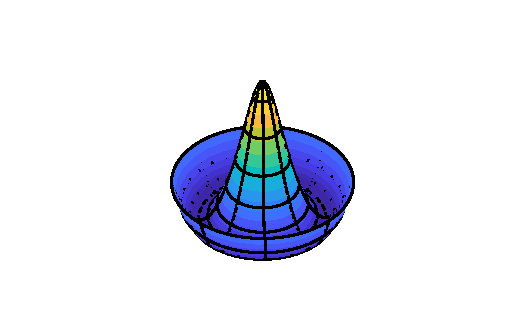
\includegraphics[width=0.9\columnwidth]{CouvPot.pdf}
\end{center}
\label{fig:Intro}
\end{figure}


\vfill
\hfill

\includegraphics[scale=0.25]{parisSaclay.jpg}
\pagebreak

%\vspace*{4pt}
\end{titlepage}
\pagebreak

\strut
 \thispagestyle{empty}
\newpage






% On commence le compteur de page ici
 \setcounter{page}{1}

\begin{flushleft}
\color{bleu}
{\fontsize{14}{14} \selectfont
	\textbf{Remerciement}}\\

\color{black}
\end{flushleft}

\commentout{
Je souhaiterais remercier l'ensemble des membres du ... que j'ai eu le plaisir de rencontrer pour leur accueil chaleureux et leur aide tout au long de mon stage. Je souhaiterais tout particulièrement remercier Bertrand Delamotte et Nicolas Dupuis qui m'ont 
}



\begin{flushleft}
\color{bleu}
{\fontsize{14}{14} \selectfont
	\textbf{Acknowledgments}}\\

\color{black}
\end{flushleft}
\commentout{
I would like to thank all the members of LPTMC whom I had the pleasure to meet for their warm welcome and their help. I would particulary like to thank ... who has helped and guided my with the project as well as the administrative procedures.
}
\vspace*{11pt}



\begin{center}
\rule{13.7cm}{.5pt}
\end{center}

\vspace*{-11pt}
\begin{abstract}

 -- Abstract non fini d'un ancien rapport, à changer -- \\
Nous montrons qu'un ensemble d'atomes froids isotropes dans un réseau optiques 2D peut permettre de stocker de la lumière sur des temps sous-radiant à l'aide d’interactions dipolaires collectives. Nous excitons les dipôles atomiques dans le plan du réseau par une lumière plane monochromatique proche résonance puis en manipulant correctement les niveaux d'énergie atomiques par effet Zeeman nous avons réussi à tourner les y rendre perpendiculaire. En réalisant un traitement exact sur des réseaux réalistes nous obtenons des temps d'émission spontané collectifs d'environ huit fois le temps d’émission spontané d'un atome unique. Nous montrons aussi que les distances interatomiques et la taille du réseau jouent un rôle important pour augmenter ce temps ; un total de 400 atomes étant suffisant pour obtenir la sous-radiance annoncée. De plus il serait très avantageux de parvenir à créer des réseaux avec un meilleur confinement des atomes puisque pour un confinement parfait nous obtenons un stockage cent fois plus long qu'avec un atome unique. Enfin l'étude de la transmission de la lumière diffusée met en avant les résonances du système ainsi que la possibilité de l'utiliser comme détecteur de champ magnétique. 
\end{abstract}

\begin{center}
\rule{8cm}{.5pt}
\end{center}


\renewcommand{\abstractname}{Abstract}
\begin{abstract}
We show that an atomic ensemble of colf atom in a 2D lattice can be used to store light on subradiant times thanks to dipole-dipole collective interactions. We exite dipole moments in the plane of the lattice with a near resonant plane monochromatic weak light and accurately handling the atomic levels with Zeeman effect we manage to spin them to be oriented perpendicularly and trap the photons. We realized an exact treatment with realistic lattices parameters and found a collective linewidth up to eight times less the linewidth of a single atom. We show that the lattice-spacing and the number of atoms has a important impact on that collective linewidth and a that a lattice of 400 atoms is large enough to reach the previous subradiance. Moreover it would be beneficial to create lattice confinment of the atomes even stronger that what is experimentally currently possible since a perfect confinement gives linewidths greater that one hendred times the linewidth of a single atom. Eventually the study of the transmission showed the system resonances and the possibility to use it as a weak magnetic field detector.  
\end{abstract}


\begin{center}
\rule{13.7cm}{.5pt}
\end{center}

\pagebreak 

\tableofcontents

\pagebreak
\begin{multicols}{2}

\section{Introduction}

\subsection{Physique statistique}

La physique statistique établit un cadre permettant de calculer les grandeurs macroscopiques, dites aussi thermodynamiques, des problèmes mettant en jeu des systèmes avec un très grand nombre de degrés de liberté en interaction. Pour donner une image de ce que cela signifie, on considère un litre d'eau enfermé dans une boite. Ce litre d'eau est constitué de $\sim 10^{24}$ molécules qui peuvent vibrer, se déplacer ou tourner dans les trois directions de l'espace et avec une certaine vitesse. La position d'une seule de ces molécules représente trois degrés de libertés (un pour chaque projection de la position dans l'espace à trois dimensions) du système total, son orientation, ou sa vitesse aussi, etc. On remarque alors que, un seul litre d'eau, possède un nombre colossal de degrés de libertés qui peuvent interagir ensembles (ici par l'intermédiaire, entre autre, des collisions des molécules). Il n'est donc pas possible de déterminer les propriétés physiques macroscopiques de ce système en étudiant la dynamique individuelle de chaque degré de liberté le constituant, ce pourquoi on a recours aux statistiques. 

Nous allons nous intéresser ici plus particulièrement à un domaine particulier de la physique statistique et de la thermodynamique qu'est l'étude des transitions de phase. Pour cela commençons par décrire ce dont il s'agit, puis nous expliciterons ce que que nous allons y étudier. \\


\subsection{Transitions de phases}

En thermodynamique on appelle phase un milieu possédant des propriétés physiques et chimiques homogènes. Or, avec la modification de certains paramètres (comme la température, la pression, etc.), un système peut changer de phase ; il se produit alors une transition de phase. Ceci est dû à une réorganisation, au niveau microscopique, des constituants  du système (molécules, atomes, ...), ayant un effet macroscopique. Landau a classé ces transitions suivant deux types : celles du premier ordre et celles du second \cite{toledano1987landau}. La distinction se fonde sur la continuité ou non de certaines fonctions thermodynamiques, définies sur le système, au moment de la transition.
 
Le passage de l'eau de l'état liquide à l'état gazeux par modification de la température extérieure à pression constante est un example de transition du premier ordre \footnote{Il est possible de définir une chaleur latente à la transition, comme la quantité d'énergie qu'il faut fournir à un volume d'eau à 100°C à pression ambiante pour passer entièrement dans la phase gazeuse. Toute l'eau ne passe pas instantanément de la phase liquide à la phase gazeuse. Ceci est associé à la discontinuité d'une fonction de la température nommé le paramètre d'ordre.}. 
\commentout{ En effet un volume d'eau pure à pression ambiante soumis à une température extérieure de plus de 100°C boue. Cependant pendant cette transition de phase entre l'état liquide et l'état gazeux l'eau liquide en elle même se maintient à une température constante de 100°C exactement avant de s'évaporer. L'énergie du système augmente donc progressivement en recevant de la chaleur du milieu extérieur mais la température du liquide ne varie pas, on dit que le système emmagasine cette énergie sous forme de chaleur latente. Ce comportement est lié à la discontinuité de certaines fonctions thermodynamiques et est donc un point caractéristique des transitions du premier ordre.}
D'un autre côté, un métal aimanté à température ambiante qui n'est soumis à aucun autre champ magnétique extérieur voit son aimantation disparaitre lorsque lorsqu'il est chauffé au dessus d'une certaine température. Ceci est aussi une transition de phase, en revanche, elle est du second ordre \cite{kochmanski2013curie}. On s'intéresse plus particulièrement ici aux phénomènes physiques qui se produisent lors des transitions du second ordre. \\

Pour comprendre quels sont ces phénomènes considérons (comme dans toute la suite de cette étude) un système que l'on peut faire changer de phase en variant sa température $T$ uniquement. On appelle $T_c$, température critique, la température à laquelle se produit la transition. Il est alors possible de définir sur ce système une fonction de corrélation $G^{(2)}(r)$ qui décrit quantitativement l'influence que deux degrés de libertés du système séparés d'une distance $r$ ont l'un sur l'autre. Notons bien que plus la distance entre les deux sera grande moins cette influence sera forte et donc plus la fonction de corrélation sera faible. A cette fonction, qu'il est possible de déterminer expérimentalement \cite{Bellac2012}, on y associe une longueur $\xi$ qui définit approximativement la distance à partir de laquelle deux degrés de libertés du système n'ont plus d'influence l'un sur l'autre.\\

On observe expérimentalement qu'au moment d'une transition de phase du second ordre, pour $|T-T_c| \rightarrow 0$, à la fois $\xi$ et $G^{(2)}$ divergent, selon les lois 
\begin{equation}
	\xi \widesim{} |T-T_c|^{-\nu} 	\quad \text{et} \quad G^{(2)}(r) \widesim{r \to \infty} |r|^{2-d-\eta},
\end{equation}
où $d$ est la dimension physique du système et $\nu$ et $\eta$ sont deux réels positifs appelés les \emph{exposants critiques}. Notons qu'il existe aussi comme cela plusieurs autres grandeurs desquelles ont peut extraire différents exposants critiques. Le point essentiel étant que tous les systèmes ayant les mêmes propriétés de symétrie possèdent les mêmes exposants critiques, on dit qu'ils appartiennent à la même classe d'universalité. En outre, un système possède une certaine symétrie lorsque l'action de celle-ci sur les degrés de liberté n'en change pas l'énergie. Nous détaillons plus en détails en \refsec{ON} à quoi correspond la symétrie $O(N)$ à laquelle nous nous sommes intéressés. 

L'avantage est qu'il suffit alors d'étudier un système 'jouet' très simple, le plus simple possible, ayant la symétrie souhaitée pour trouver les exposants critiques de tous les autres systèmes physiques plus complexes avec la même symétrie. Notons que la température critique $T_c$ n'est pas une grandeur universelle,elle est propre à chaque système et varie d'un système à l'autre, même s'ils ont les mêmes symétries. Pour la calculer il n'est donc pas possible d'utiliser l'astuce précédente, il faut étudier précisément le système d'intérêt.


\subsection{Intérêt du groupe de renormalisation et des équations BMW}

Le groupe de renormalisation (RG) permet de montrer l'effet d'universalité des exposants critiques et de les calculer. L'approche par le RG a permis d'obtenir déjà d'excellents résultats \cite{kadanoff1967scaling, wilson1971renormalization2} pour différents systèmes étudiés comparé aux expériences et autres méthodes comme les simulations Monte-Carlo. Cependant elle reste limitée dans ces applications car elle se fonde sur des approximations de "théorie des perturbations" qui ne permettent de ne calculer par exemple que les exposants universels critiques mais pas les grandeurs non universelles comme la température critique $T_c$.\\

Le groupe de renormalisation non perturbatif (NPRG) permet de répondre à ce problème en reprenant le principe du RG sous une approche différente permettant d'accéder à des équations exactes. L'inconvénient est qu'alors ces équations exactes n'ont pas de solution a priori. Il faut faire d'autres approximations, comme l'approximation BMW, pour obtenir des équations solubles numériquement. Bien que cela reste compliqué en pratique, ces approximations peuvent alors permettre de récupérer à la fois les exposants critiques et la température critique. \\

Le but de cette étude est d'appliquer l'approximation BMW à des systèmes dont exposants et température critiques sont connus grâces à d'autres méthodes exactes ou numériques, afin de valider la qualité de cette approximation et de la résolution numérique.\\
\indent
Nous avons repris une simulation numérique d'équations intégro-différentielles non linéaires obtenues par l'approximation BMW pour des systèmes régis par une certaine symétrie dite $O(N)$ à l'aide du système modèle générique de la "théorie $\varphiv^4$" \cite{LeonardThesis}. Elle a déjà permis de déterminer des exposants critiques avec précision pour certains systèmes, mettant bien en avant la qualité de l'approximation BMW. Cependant elle présente des comportements étranges et des résolutions instables dans d'autres cas. Le but était donc d'en rechercher les causes pour parvenir enfin à calculer avec ce code les exposants $\eta$ et $\nu$ dans toutes les configurations.\\
\indent
De plus nous avons aussi réalisé la simulation des équations BMW pour un modèle précis, nommé Ising en deux dimensions (Ising 2D), ayant une symétrie $O(N=1)$, afin d'essayer d'en récupérer la température critique et de la comparer à la valeur théorique connue. L'objectif est alors bien de valider la justesse de l'approximation BMW, en montrant sa capacité à calculer numériquement une grandeur non universelle, $T_c$, d'un système donné. \\

Dans une première partie nous rappelons les origines du modèle du RG et du NPRG puis nous l'utilisons pour expliquer la structure des équations BMW dans le cas de de la théorie $\varphiv^4$ et étudier numériquement leur résolution et la recherche des exposants critiques associés. Enfin nous introduirons le modèle d'Ising à deux dimensions et les simulations numériques que nous avons réalisé dessus. 


\vspace*{11pt}



\section{Origine du modèle}
\subsection{Concepts de physique statistique}

\label{sec:Origin}

Nous résumons dans cette sections quelques concepts fondamentaux de la thermodynamique et de la physique statistique \cite{diu2007thermodynamique} nécessaires à l'introduction du groupe de renormalisation. \\

Considérons un système à $P$ corps dans un ouvert à $d$ dimensions $\Omega$ de volume $|\Omega|$. Chacun de ces $P$ corps possèdent $N$ degrés de liberté. On considère que l'ensemble des $N$ degrés de liberté de chacun de ces $P$ corps peuvent être décrit suivant leur position $\rv$ grâce à une fonction $\varphiv : \rv \in \Omega \rightarrow \varphiv(\rv) \in \R^N$, telle que $\varphiv \in \( \Cc^{0}(\Omega)\)^N$. Si un corps se situe en $\rv$ les $N$ composantes du vecteur $\varphiv(\rv)$ représentent alors chacune la valeur de l'un de ces degrés de liberté. \\

\commentout{
 ensemble de vecteurs $\{{\varphiv_\rv}\}_\rv$. Le vecteur $\varphiv_\rv$ possède $N$ composantes représentant chacune la valeur d'un degré de liberté du corps situé en $\rv$. Cependant comme nous en avons déjà discuté, nous étudions des systèmes macroscopique, ou autrement dit, des systèmes dans la limite thermodynamique où le nombre $P$ de corps est très élevé. Suffisamment élevé pour considérer que l'ensemble de valeurs ${\{{\varphiv_\rv}\}}_\rv$ discrètes peut en réalité s'exprimer comme une fonction $\varphiv : \rv \in \Omega \rightarrow \varphiv(\rv) \in \R^N$, telle que $\varphiv \in \( \Cc^{0}(\Omega)\)^N$. }

La dynamique du système est alors régie par un une fonctionnelle de $\varphiv$ : l'hamiltonien $H[\varphiv]$\footnote{Pour être plus précis ici $H = \beta H_\text{stat}$, où $\beta = 1/(k_b)T$ et $H_\text{stat}$ est classiquement le hamiltonien de la physique statistique}. Avec le formalisme canonique de la physique statistique \cite{rohtuA} nous savons que nous pouvons connaitre toutes l'information sur les propriétés macroscopiques du système en étudiant sa fonction de partition $\Zc$ définie par l'expression 
\begin{equation}
\Zc \equiv \int \Dc \varphiv \, \exp\left\{- H[\varphiv]\right\}, 
\end{equation} 
Cette intégrale est une intégrale fonctionnelle \cite{} sur l'ensemble des champs $\varphiv$ permis par le système (i.e. une somme continue sur l'ensemble des configurations possibles des $P\times N$ degrés de liberté du système). Cependant elle ne peut pas être, de manière générale, calculée pour un $H$ quelconque.\\

Considérons l'hypothèse physique selon laquelle $H$ peut se décomposer en deux parties distinctes,
\begin{equation}
H[\varphiv] = S[\varphiv] - \int_{\Omega} \hv \varphiv,
\end{equation} 
où $S$ est l'hamiltonien du système non excité et le deuxième terme correspond à l'excitation du système par un champ $\hv$ extérieur. Ainsi $\Zc$ devient une fonctionnelle de $\hv$ et nous définissons l'énergie libre du système selon 
\begin{equation}
  W[\hv] = \text{ln}{\(\Zc[\hv]\)}
\end{equation}
En utilisant la notion de dérivée fonctionnelle nous pouvons alors introduire $G^{(n)}$ le tenseur des fonctions de corrélations à $n \in \bbrac{1,N}$ corps. Ces fonctions sont très importantes car, comme mentionné dans l'introduction, c'est celle à deux corps qui nous permet de déterminer les exposants critiques $\nu$ et $\eta$. Pour $j \in \bbrac{1,n}$, on pose $\{i_j\} \subset \bbrac{1,N}$ avec $\text{card}(\{i_j\}) = j$. 
\begin{equation}
  G^{(n)}_{\{i_j\}} [\{\rv_{j}\} ; \hv] = \derd{^n W[\hv]}{h_{i_1}(\rv_1) ... \delta h_{i_n}(\rv_n)}
\end{equation}
Cependant ces grandeurs ne peuvent pas se calculer directement. Or, comme l'énergie libre est une fonction convexe \cite{diu2007thermodynamique} on peut définir, une grandeur que l'on parviendra à calculer, le potentiel Gibbs, défini par transformation de Legendre selon 
\begin{equation}
  \Gamma [\phiv] = - W[\hv] + \int_{\Omega} \hv \phiv,
\end{equation}
Avec, en notant $\left< ... \right>$ la moyenne statistique, et en introduisant le champ moyen $\phiv$,
\begin{equation}
  \phiv[\rv, \hv] = \left< \varphiv(\rv) \right> = \derd{W[\hv]}{\hv(\rv)}
\end{equation}
\begin{equation}
  \left< \varphiv(\rv) \right> = \frac{1}{\Zc} \int \Dc \varphiv \, \varphiv(\rv) \exp\left\{- H[\varphiv]\right\}, 
\end{equation}
On introduit aussi une notation pour les tenseurs de dérivées fonctionnelles de $\Gamma$ avec 
\begin{equation}
  \Gamma^{(n)}_{\{i_j\}} [\{\rv_{j}\} ; \phiv] = \derd{^n \Gamma[\phiv]}{\phi_{i_1}(\rv_1) ... \delta \phi_{i_n}(\rv_n)}
\end{equation}
On montre alors \cite{Delamotte2012}, qu'au sens d'inverse d'opérateur, comme définie en annexe,
\begin{equation}
  G^{(2)}[\hv] = \(\Gamma^{(2)}[\phiv]\)^{-1}  
\end{equation}

Il faut donc retenir que la connaissance du potentiel de Gibbs équivaut à la connaissance de la fonction de corrélation à deux points qui nous permet alors aussi de retrouver les exposants critiques qui nous intéressent. 

\begin{figure}[H]
\begin{center}
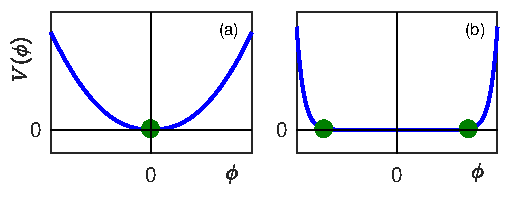
\includegraphics[width=0.95\columnwidth]{CourbePot1.pdf}
\caption{Allure du potentiel pour un champ n'ayant qu'une seule composante : $\phiv = \phi$. La position de $\phi_m$ est symbolisée par les points verts. Dans le cas (a), nous sommes dans la phase dite haute température. Dans le cas (b) le potentiel est toujours une fonction convexe mais elle est extra plate autour de l'origine. En physique on dira que le minimum de V ne se trouve pas vraiment en $0$ mais sur les bords de la région plate, suivant certains critères. Remarquons qu'il s'agit bien alors de fonctions concaves et paires.}
\end{center}
\end{figure}
\vspace*{-11pt}

En outre la connaissance de $\Gamma[\phiv]$ a aussi un autre avantage important puisque si l'on prend $\phiv$ comme une fonction uniforme alors $\phiv$ est une grandeur ne dépendant plus de $\rv$ et $\Gamma$ devient une fonction (et non plus une fonctionnelle). Or à un facteur de volume $|\Omega|$ près, $\Gamma$ correspond alors au potentiel du système que l'on note $V$ selon :
\begin{equation}
	V(\phiv) = \frac{1}{|\Omega|}{\left. \Gamma[\phiv] \right|}_{\phiv \text{ unif.}},
\end{equation}
et la position du minimum global de $V$ noté $\phiv_m$ est lié à la nature de la phase dans laquelle se trouve le système. Si jamais $\phiv_m \neq 0$ alors la température du système est inférieure à la température critique : on dit qu'il est dans la phase basse température. En revanche si  $\phiv_m = 0$ la température est au dessus de la température critique et le système est dans la phase haute température.\\



\subsection{La symétrie $O(N)$}

\label{sec:ON}

On dit qu'un système est symétrique selon $O(N)$ s'il est invariant par l'action du groupe de rotation $O(N)$ sur ces degrés de libertés. Plus précisément, soit $J \in O(N)$, et on note $J.V$ l'action de $J$ sur un vecteur $V$ de $\R^N$. Le modèle est dit $O(N)$ si 
\begin{equation}
	H[J .\varphiv] = H[\varphiv]	
\end{equation}
Dans la suite nous utiliserons alors une autre grandeurs scalaire invariante sous $O(N)$ pour caractériser les champs $\phiv$ uniformes 
\begin{equation}
	\rho = \frac{1}{2}  \phiv^2  
\end{equation}
Ainsi, pris en $\phiv$ uniforme le potentiel effectif $\Gamma^{(2)}$ par exemple devient une fonction de $\rho$ qui est un salaire et plus un vecteur comme $\phiv \text{ unif.}$ l'est. Il en est pour $V$ ou tout autre grandeur fonction de $\phiv$. Notre étude porte uniquement sur des systèmes possédant cette symétrie.\\

Développons à présent les concepts du RG et du NPRG avec lesquels nous avons travaillés.



\vspace*{11pt}
\subsection{Le groupe de renormalisation (RG)}


\subsubsection{Transformée de Fourier}

\label{sec:TF}

Nous rappelons ici de manière synthétiques les principales idées du RG développé par Wilson \cite{wilson1971renormalization, wilson1971renormalization2,fisher1998renormalization}. Commençons pour cela par définir la transformée de Fourier du champ $\varphiv$ appartenant à $L^2(\Omega)$ par 
\begin{equation}
\begin{split}
\hat{\varphiv}_\pv = \frac{1}{\sqrt{|\Omega|}}\int_\Omega \varphiv(\rv) \, e^{-i \pv . \rv} \dd \, \rv, \\
\varphiv(\rv) = \frac{1}{\sqrt{|\Omega|}}\sum_\pv \hat{\varphiv}_\pv \, e^{i \pv  .\rv}
\end{split} 	
\end{equation}
On fait l'hypothèse qu'il existe un réel $\Lambda$ tel que pour $\|\pv\|_{\infty} > \Lambda$, $\hat{\varphiv}(\pv) \simeq 0$. On considère donc $\pv \in [0, \Lambda]^d$. Ceci signifie que $\varphiv$ est une fonction suffisamment régulière et cette valeur $\Lambda$ correspond physiquement à l'inverse de la plus petite longueur caractéristique du système, qui est classiquement la distance moyenne entre les corps par exemple. En pratique on suppose que comme dans la limite thermodynamique on étudie des systèmes macroscopiques tels que $|\Omega|\gg 1/\Lambda^d$. Ainsi on fait l'approximation physique selon laquelle les impulsions ne sont plus des variables discrètes mais continues avec les équivalences  

\begin{equation}
\begin{split}
	\frac{1}{|\Omega|} \sum_{\pv} & \rightarrow \frac{1}{(2\pi)^d} \int_{\R^d} ... \, \dd \, \pv  \equiv \int_\pv ... \\
	\int_\Omega	... \, \dd \, \rv & \rightarrow \int_\R ... \, \dd \rv \equiv \int_\rv ...
\end{split}
\end{equation}
Pour $\varphiv$ fixé la suite $\hat{\varphiv}_\pv$ dans $\ell^2$ devient une fonction $\hat{\varphiv} : \pv \rightarrow \hat{\varphiv}(\pv)$ de $L^2(\R)$. 
Remarquons aussi que si $\hat{H}$ est la transformée de Fourier de $H$ alors nous avons toujours
\begin{equation}
\Zc = \int \Dc \hat{\varphiv} \, \exp\left\{- \hat{H}[\hat{\varphiv}]\right\}. 
\end{equation} 
Dès lors qu'il n'y aura pas d'ambiguïté possible, nous pourrons donc oublier à partir de maintenant la notation avec le chapeau en notant que c'est la variable utilisée $\rv$ ou $\pv$ (ou aussi parfois $\qv$ pour l'impulsion) qui nous permet de savoir si l'on travaille avec la fonction considérée ou sa transformée de Fourier. \\


\subsubsection{Idée générale}

\label{sec:RG}

L'idée du RG est alors de ne pas considérer tous les degrés de liberté sur le même pied d'égalité. En effet, on commence d'abord, pour calculer $\Zc$, par intégrer les degrés de libertés de haute impulsion $\pv$ entre $k = \Lambda/s$ et $\Lambda$ où $k \in [0,\Lambda]$. En pratique on sépare $\varphiv$ en deux fonctions $\varphiv_>$ et $\varphiv_<$ telles que $\varphiv(\pv) = \varphiv_{k,>}(\pv) + \varphiv_{k,<}(\pv)$ et
\begin{align}
	\varphiv_{k,>}(\pv)  = \quad & \varphiv(\pv) \quad \text{si} \quad \pv \in   [k,\Lambda] \\
	 & 0 \quad \text{sinon}
\end{align}
Ceci permet de définir un Hamiltonien effectif $H_k$, 
\begin{equation}
	H_k[\varphiv_{k,<}] \equiv \int \Dc \varphiv_{k,<}  \exp \{ H[\varphiv_{k,>}+ \varphiv_{k,<}] \},
\end{equation}
et de réécrire la fonction de partition comme 

\begin{equation}
\Zc = \int \Dc \varphiv_{k,<} \, \exp\left\{- H_k[\varphiv_{k,<}]\right\}. 
\end{equation} 

De manière générale on part d'un hamiltonien qui ne dépend pas seulement du champ $\varphiv$ mais entendu aussi de constantes de couplage qui caractérisent la physique à laquelle est soumise le champ. Ces constantes sont notées $\{g_i\}_i$ avec $i \in \N$. On écrit alors $H[\varphiv] = H[\varphiv ; \{g_i\}]$. Le nouvel hamiltonien $H_k[\varphiv_{k,<}]$ peut alors s'exprimer aussi sous la forme $H_k[\varphiv_{k,<} ; \{g_{k,i}\}_i]$ où $\{g_{k,i}\}_i$ sont de nouvelles constantes de couplages. \\

Bien entendu il n'est pas directement possible de calculer $H_k$ pour $k$ quelconque, sinon le problème serait résolu en calculant $H_0$. On considère alors plutôt une intégration infinitésimale entre $[\Lambda - d\Lambda, \Lambda]$ pour obtenir le nouvel hamiltonien $H_{k_1}$, où $k_1 = \Lambda - d\Lambda$. On introduit aussi $s_1 = \Lambda/k_1$. Ce calcul là, contrairement au calcul direct pour $k$ quelconque, peut être réalisé grâce à des approximations comme nous le détaillerons ensuite. Maintenant, avec l'expression de ce nouvel hamiltonien, on réalise ce que l'on appelle un adimensionnement qui se déroule en trois étapes listées ci-dessous.

 Tout d'abord, comme $\pv$ est homogène à $\text{L}^{-1}$ (ou L est la dimension d'une longueur) on introduit $\tilde{\pv} = s_1 \pv$. Ensuite on montre que le champ $\varphiv_{k_1, <}$ est homogène à $\text{L}^{d-2-\eta}$ (avec $\eta$ l'exposant critique défini dans l'introduction), on pose donc $\tilde{\varphiv}_{k_1, <}$ tel que $\varphiv_{k_1, <}(\pv) = s_1^{-d+2+\eta} \tilde{\varphiv}_{k_1, <}(\tpv)$ pour tout $\pv \in [0, \Lambda]^d$. Enfin la constante $g_{k_1, i}$ pour tout $i\in \N$ est aussi homogène à $\text{L}^{b_i}$ avec $b_i$ une constante. On écrit donc de nouvelles constantes de couplage $\{\tilde{g}_{k_1, i}\}_i$ telles que $g_{k_1, i} = s_1^{-b_i} \tilde{g}_{k_1, i}$. Ceci définit un hamiltonien $\tilde{H}$,
 \begin{equation}
 	\tilde{H}_{k_1}[\tilde{\varphiv}_{k_1,<}; \{\tilde{g}_{k_1, i}\}_i ] = H_{k_1}[\varphiv_{k_1,<}; \{g_{k_1,i}\}_i]
 \end{equation}
La fonction de partition (dont il ne sert en fait à rien de connaitre le préfacteur numérique) est alors simplement exprimée comme 
\begin{equation}
\Zc \propto \int \Dc \tilde{\varphiv}_{k_1,<} \, \exp\left\{- \tilde{H}_{k_1}[\tilde{\varphiv}_{k_1,<}, \{\tilde{g}_{k_1, i}\}_i ] \right\}. 
\end{equation} 


Ce changement est purement technique cependant il a un fondement physique puisqu'il permet de faire comme si $\tilde{H}_{k_1}$ était l'hamiltonien d'un "nouveau système" identique au système originel étudié mais dans lequel toutes les échelles d'impulsion ont été dilatées d'un facteur $s_1$ et les échelles de longueur alors réduites d'un facteur $s_1$. Or on rappelle que pour une transition de phase du second ordre la longueur $\xi$ du système originel diverge. Ce "nouveau système" possède alors une longueur de corrélation $\xi_1 = \xi/s_1$ qui diverge aussi à la transition : $\xi, \xi_1 \to \infty$. Ainsi, à la transition de phase, et uniquement à la transition, les deux systèmes possèdent la même physique. En effet, si $\xi$ ne divergeait pas (et donc si l'on n'était pas à la transition de pas) ce ne serait pas le cas puisque alors $\xi_1 \neq \xi$, et deux systèmes avec des longueurs de correléations différentes, ne représenteraient pas la même chose. \\

 Pour réaliser l'intégration complète sur $[0, \Lambda]$ on peut donc ensuite itérer ce processus de transformations infinitésimales en repartant de l'expression de $\Zc$ en fonction de $\tilde{H}_{k_1}[\tilde{\varphiv}_{k_1,<}, \{\tilde{g}_{k_1, i}\}_i ]$. On reproduit le même procédé, par exemple au deuxième pas de l'itération, en calculant l'intégration infinitésimale entre $[\Lambda - 2d\Lambda, \Lambda - d\Lambda]$ avec $k_2 = \Lambda - 2d\Lambda$. A la fin de cette deuxième itération nous avons donc intégré sur $[\Lambda - 2d\Lambda, \Lambda]$.  \\
 
 On introduit alors à l'itération $p \in \N$ - itération à laquelle on a intégré sur $[k_p, \Lambda]$ - l'opérateur $O_p$ qui envoie $\{\tilde{g}_i\}_i$ sur $\{\tilde{g}_{k_p,i}\}_i$. L'hypothèse fondamentale du RG, qui n'est pas prouvée mais toujours vérifiée, est qu'il existe un point fixe de $O_p$ pour $p \to \infty$, si l'on est à la température critique (et/ou pression critique, ...). Ceci signifie plus exactement qu'il existe $\{\tilde{g}^*_i\}_i$ tel que 
 \begin{equation}
 	\lim\limits_{k \rightarrow \infty}  \tilde{g}_{k,i} = \lim\limits_{\substack{p \to \infty \\ d\Lambda \to 0 }}  \tilde{g}_{k_p,i} =  \tilde{g}^*_i
 \end{equation} 
Sans entrer plus en profondeur dans les calculs du RG on admet que l'on peut montrer que l'existence de ce points fixe explique alors l'universalité de exposants critiques \cite{Delamotte2012}. En effet, deux systèmes avec les mêmes propriétés de symétries auront le même point fixe, ce qui revient à dire d'une autre manière qu'ils auront bien un comportement, une physique, identique à la transition de phase, quand la longueur de corrélation est infinie. \\
 
Dans un calcul de RG on prend classiquement un nombre fini de constantes de couplage et on considère qu'elles sont suffisamment faibles pour faire des développement du hamiltonien en puissance de ces constantes adimensionnées à chaque itération. Ce sont ces approximations qui permettent de faire des calcul mais elles limitent les applications possibles. Le NPRG développe alors une technique reprenant la même idée de calcul mais sans faire ces approximations, grâce à une astuce.

\vspace*{11pt}
\subsection{Le groupe de renormalisation non perturbatif (NPRG)}
\subsubsection{Généralités}

Contrairement au RG le NPRG développé par Wetterich \cite{wetterich} va plus loin puisqu'il permet un calcul sans approximations a priori. L'idée reste la même que dans le RG en intégrant les hautes impulsions en  premier lieu. Cependant l'astuce consiste à faire cela en introduisant un tenseur de fonctions  $\Rc \in \(H_1(]0, \Lambda[^{d+1})\)^{N\times N} : (k,\qv) \to \Rc_{k, ij}(\qv)$, puis une nouvelle fonction de partition modifiée,  
\begin{equation}
  \Zc_k[\hv] = \int \Dc \varphiv \, \exp\left\{-S[\varphiv] - \Delta S_k[\varphiv] + \int_{\rv} \hv \varphiv \right\} \, ,
\end{equation}
avec la définition
\begin{equation}
  \begin{split}
  \Delta S_k[\varphiv]  & \equiv \frac{1}{2} \int_{\rv, \rv'} \varphi_i(\rv) \Rc_{k,ij}(\rv - \rv') \varphi_j(\rv') \\
 & =  \frac{1}{2} \int_{\qv} \varphi_i(-\qv) \Rc_{k,ij}(\qv) \varphi_j(\qv)
\end{split}
\end{equation}
C'est grâce à l'évolution de $\Rc_{k,ij}$ en fonction de $k$ que l'on intègre au fur et à mesure les degrés de liberté. En effet, dans l'esprit du RG, on souhaite retrouver $\lim_{k \to 0}\Zc_k = \Zc$ et pour $k = \Lambda$ que l'expression de $\Zc_\Lambda$ puisse être calculée analytiquement. De cette manière, en faisant évoluer $k$ de $\Lambda$ à $0$ on peut suivre l'évolution de $\Zc_k$ d'une valeur connue à la valeur $\Zc$ par le biais d'une équation différentielle. On peut donc choisir $\Rc_{k,ij}$ tel que \\

\begin{itemize}
  \item (C1) Pour $k \rightarrow 0$, $\forall \qv$ $\, \Rc_{k, ij}(\qv) \rightarrow 0$  .
  \item (C2) Pour $k = \Lambda$, $\forall \qv$ $\, \Rc_{k, ij}(\qv)  \rightarrow  +\infty$ .
\end{itemize}
\vspace*{11pt}

Et il faut que l'évolution entre ces deux configurations soit continue. Etant donné que numériquement nous ne pouvons pas prendre en compte $\Rc_{k, ij}$ allant vers l'infini quand $k = \Lambda$ nous nous contenterons de prendre $\Rc_{\Lambda, ij}$ comme une fonction minorée par une valeur bien supérieure aux valeurs de constantes de couplage de $H$. En pratique il suffit de prendre $\Rc_{\Lambda, ij} \sim \Lambda^2$.

Ainsi, quand $k \to 0$, $\Delta S_k \to 0$ et l'on retrouve bien l'expression de $\Zc$. De plus quand $k = \Lambda$ prendre $\Rc_{k,ij}$ comme étant très grand permet faire une excellente approximation de point-selle et écrire
\begin{equation}
	Z_\Lambda[\hv] \propto \exp\left\{-S[\varphiv_0] - \Delta S_k[\varphiv_0] + \int_{\rv} \hv \varphiv_0 \right\} 
	\label{eq:MeanZ}
\end{equation}
Ou l'on définit $\varphiv_0$ par 
\begin{equation}
	{\left. \derd{\(S[\varphiv] + \Delta S_k[\varphiv]\)}{\varphiv} \right|}_{\varphiv_0 \text{ unif.}} = \hv
	\label{eq:meanPhi}
\end{equation}
L'intégrale a alors disparue dans l'expression de $Z_\Lambda$, qui s'exprime uniquement en fonction d'un champ bien défini $\varphiv_0$. De cette manière on dit que l'on "gèle les fluctuations" du champ autour de $\varphiv_0$ et on peut calculer analytiquement $\Zc_\Lambda$. \\

Enfin, il faut aussi que $\Rc_{k,ij}$ soit une fonction possédant des symétries compatibles avec le système que l'on considère pour pouvoir effectuer des calculs.


\vspace*{11pt}

\subsubsection{Choix du régulateur}
\label{sec:Reg}

Dans le modèle $O(N)$ il suffit de prendre $\Rc_{k,ij} = \Rc_k$ comme une simple fonction et pas un tenseur. De plus en guise d'illustration (et parce que cela correspond bien à ce que nous avons utilisé par la suite dans le cas de la théorie $\varphiv^4$) nous considérons que $\Rc_k(\qv) = \Rc_k(q)$ avec $q = \|\qv\|_2$ la norme 2 dans $\R^d$. La fonction $(k,q) \to \Rc_k(q)$ est appelée le régulateur.


\begin{figure}[H]
\begin{center}
	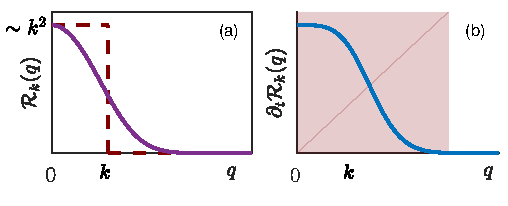
\includegraphics[width=0.95\columnwidth]{RegDerReg.pdf}
\end{center}
\vspace*{-22pt}
\caption{(a - bleu continue) Allure du régulateur, choisi pour une valeur de $k$ donnée, ayant une décroissance exponentielle entre $\simeq k^2$ et $0$. (b - rouge pointillé) régulateur avec une "décroissance" discontinue vers $0$ à grand $q$ que l'on peut exprimer avec une fonction de Heaviside. Ainsi ici nous avons approximativement intégrés les degrés de libertés correspondant à une impulsion dans $\simeq [k,\Lambda]$ uniquement. (b) Allure de la dérivée temporelle du régulateur choisi pour une valeur de $k$ donnée avec une décroissance exponentielle (ligne continue bleue). L'intégrale sur $\qv$ dans \refeq{} ne doit donc être faite seulement sur les $q$ appartenant dans la région rouge.}
\label{fig:RegDerReg}
\end{figure}


Nous choisirons le régulateur ayant l'allure de ceux présent sur la figure \refig{RegDerReg} (a), pour $k$ fixé, afin de satisfaire à tous les critères. Les deux régulateurs exposés sont équivalents, même si celui qui est discontinu peut entrainer des instabilités numériques.




\vspace*{11pt}
\subsubsection{Potentiels}

En réalité, ce n'est pas vraiment à $\Zc$ que nous allons nous intéresser, mais plutôt aux potentiels qui en dérive, car ils contiennent toutes les informations dont nous avons besoin. 	On reprend alors les différentes définitions données dans la section \refsec{Origin} dans le cas des notations de la limite thermodynamique $\Omega \gg 1/\Lambda^d$ (\refsec{TF}) et que l'on adapte pour prendre en compte la présence du régulateur. Tout d'abord, pour $k$ fixé, on définit une énergie libre 
\begin{equation}
	  W_k[\hv] = \text{ln}{\(\Zc_k[\hv]\)}
\end{equation}
Et de même pour le tenseur des fonctions de corrélations, que l'on exprime cette fois ci en fonction des transformées de Fourier (c.f.\refann{outils}) et en reprenant les mêmes notations qu'en \refsec{Origin}.
\begin{equation}
  G^{(n)}_{k,\{i_j\}} [\{\pv_{j}\} ; \hv] = \derd{^n W_k[\hv]}{h_{i_1}(-\pv_1) ... \delta h_{i_n}(-\pv_n)}
\end{equation}
En revanche, on ne définit plus exactement la fonctionnelle $\Gamma$ de la même façon, on ne réalise plus vraiment exactement une transformée de Legendre, mais
\begin{equation}
  \Gamma_k [\phiv] = - W_k[\hv] + \int_{\rv} \hv \phiv - \Delta S_k[\phiv],
\end{equation}
Avec $\phiv$ défini comme 
\begin{equation}
  \phiv[\pv, \hv] = \left< \varphiv(\pv) \right> = \derd{W_k[\hv]}{\hv(-\pv)}
\end{equation}
Faire une pseudo-transformée de Legendre et non un vrai transformée de Legendre dans laquelle on n'aurait pas enlevé le terme en $\Delta S_k$ est utile pour obtenir une condition initiale de nos équations (c.f. \refeq{initFlotBMW}). On s'intersse plus particulièrement alors à l'expression de $G^{(2)}_{k,ii}$ pour $i \in \bbrac{1,N}$ pris en $\{\pv, -\pv\}$. En effet seul ce cas là aura une utilité par la suite. On notera donc cette expression, pour être concis,
\begin{equation}
	G_{k,ii}[\pv; \hv] \equiv   G^{(2)}_{k, i i}[\pv, -\pv; \hv] = \derd{^2 W_k[\hv]}{h_{i}(-\pv)\delta h_{i}(\pv)}
\end{equation}
En conservant la définition équivalente à \refeq{} de $\Gamma_k^{(n)}$ mais en transformée de Fourier
\begin{equation}
\Gamma^{(2)}_{k, \{i_j\}}[\{\pv_j\}; \phiv] = \derd{^n \Gamma_k [\phiv]}{\phiv_{i_1}(-\pv_1)...\delta \phiv_{i_2}(-\pv_n)} \, ,
\end{equation}
avec, une notation équivalente pour $\Gamma^{(2)}_k$ à $G^{(2)}_k$
\begin{equation}
\Gamma^{(2)}_{k,ii}[\pv; \phiv]  \equiv \Gamma^{(2)}_{k,ii}[\pv, - \pv; \phiv] = \derd{^2 \, \Gamma_k [\phiv]}{\phiv_{i}(-\pv)...\delta \phiv_{i}(\pv)} \, 
\end{equation}
on obtient alors, au sens de l'inverse d'opérateur, 
\begin{equation}
  G_{k}[\pv ; \hv] = \(\Gamma^{(2)}_{k}[\pv, \phiv] + \Rc_k(\pv)\)^{-1} 
\end{equation}


Enfin on peut aussi définir, pour $\phiv$ uniforme, le potentiel effectif $V_k$ par
\begin{equation}
	V_k(\phiv) = {\left. \frac{1}{|\Omega|} \Gamma_k[\phiv] \right|}_{\phiv \text{ unif.}}
	\label{eq:defPot}
\end{equation}

\vspace*{11pt}


\subsubsection{Equation de flot}

On peut alors utiliser les définitions que l'on vient de poser pour extraire l'équation fondamentale du NPRG que l'on appelle l'équation de flot exacte de $\Gamma_k$. Il s'agit d'une équation valable pour $k \in ]0, \Lambda]$ décrivant l'évolution de $\Gamma$ avec $k$ lorsqu'on le fait évoluer de $\Lambda$ à $0$. On définit une nouvelle variable $t$ appelée temps du RG.
\begin{equation}
	t = \ln(k/\Lambda), \quad \text{donnant} \quad \partial_t \, ... = k\partial_k \, ...
\end{equation}
Quand $k$ varie de $\Lambda$ vers $0$, $t$ varie de $0$ vers $-\infty$, c'est donc un "temps" négatif. On montre alors
\begin{equation}
\partial_t \Gamma_{k}	[\phiv] = \frac{1}{2} \sum\limits_{i=1}^{N} \int_\qv \partial_t \Rc_k(\qv) \, G_{k, ii}[\qv; \phiv] \, ,
	\label{eq:flot}
\end{equation}
et nous avons aussi une condition initiale  en $k = \Lambda$ pour $\Gamma_k$ puisque, en définissant $\varphiv_0$ comme en \refeq{meanPhi}, d'après \refeq{MeanZ} il vient la relation
\begin{equation}
	\Gamma_\Lambda [\phiv] = S[\phiv = \varphiv_0]
	\label{eq:initFlotBMW}
\end{equation}
Ainsi, nous avons une équation différentielle avec une condition initiale connue permettant d'accéder à $\Gamma_{k \to 0} = \Gamma$. Rappelons que la connaissance de $\Gamma^{(2)}$ permet de connaitre les exposants critiques $\eta$ et $\nu$, cette équation est donc fondamentale car connaissant $\Gamma$ nous avons aussi accès à $\Gamma^{(2)}$ par dérivation.

Notons que l'intégrale dans cette équation de flot est en fait tronquée par la fonction $q \to \partial_t\Rc_k(q)$ qui pour un $k$ fixé limite, par sa décroissance, l'intervalle utile d'intégration qui n'est donc jamais véritablement faite sur un domaine infini et peut sans problème être réalisé numériquement comme illustré en \refig{RegDerReg}\, (b),  dans le cas simple ou $\Rc_k(\qv) = \Rc_k(q)$.

Le problème maintenant est que pour connaitre $\partial_t \Gamma_k$ dans cette équation il nous faudrait connaitre la dérivée seconde $\Gamma_k^{(2)}$. Cependant la seule façon de connaitre $\Gamma_k^{(2)}$ est, de façon similaire, de résoudre l'équation de flot exacte de $\Gamma_k^{(2)}$ que l'on déduit de celle de $\Gamma_k$. Or cette équation fait intervenir $\Gamma_k^{(3)}$ et $\Gamma_k^{(4)}$, que nous ne connaissons pas non plus. De même pour $\Gamma_k^{(3)}$ pour lequel il faudrait connaitre $\Gamma_k^{(4)}$ et  $\Gamma_k^{(5)}$ et ainsi de suite. On dit alors que l'équation est ouverte et n'est pas soluble telle quelle. L'approximation BMW permet de répondre à ce problème. 


\vspace*{11pt}
\subsubsection{La dimension anormale}

\label{sec:DimAnorm}

Avant de d'aborder le principe de l'approximation BMW introduisons le concept de dimension anormale. En effet nous avons mentionner que la fonction de corrélation à deux points évolue, à la transition de phase, schématiquement en $G^{(2)}[\rv_1, \rv_2; \hv] \sim |\rv_1 - \rv_2|^{2-d-\eta}$ pour $|\rv_1 - \rv_2| \to \infty$. Or cette grandeur $\eta$, qui est un exposant critique, possède aussi le nom de dimension anormale car elle viole à priori la dimension que devrait avoir $G^{(2)}$ d'une longueur à la puissance $2-d$. Pour la prendre en compte dans les équations cela ne découle donc pas naturellement des équations déjà écrite. Pour cela on remarque que cette évolution de $G^{(2)}$ implique aussi $\Gamma^{(2)}[\pv; \phiv] \sim \pv^{2-\eta}$ quand $\pv \to 0$. On introduit alors $Z_k$ une grandeur dimensionnée,
\begin{equation}
	Z_k \equiv {\left. \frac{\partial \Gamma_k^{(2)}[\pv ;\phiv]}{\partial \pv^2} \right|}_{\phiv \text{ unif.} = \phiv_0, \pv = \pv_0 }
	\label{eq:defZk}
\end{equation}
Où $\phi_0$ et $\pv_0$ sont des valeurs arbitraire du champ uniforme et de l'implusion. De cette manière  quand $k \to 0$ nous avons $Z_k \propto \pv^{-\eta}$.
On introduit alors $\eta_k$ tel que
\begin{equation}
	\eta_k = -k \partial_k \ln(Z_k)
\end{equation}
Ainsi nous dirons que $\Gamma^{(2)}_k$ n'a pas vraiment la dimension de $\pv^2$ mais la dimension de $Z_k\pv^2$. Il est prouvé \cite{} que ce faisant 
\begin{equation}
 	\lim\limits_{k \to 0} \eta_k  = \eta
 \end{equation}
Ceci est d'une très grande importance pour l'adimensionnement des équations qui est nécessaire pour trouver les points fixes du RG (c.f. \refsec{RG}). Mais de plus c'est cette grandeur qui va donne l'exposant critique $\eta$ que l'on recherche quand $k \to 0$.


\vspace*{11pt}
\subsubsection{La recherche de points fixes}

Le but est toujours de trouver la valeur des exposants critiques des systèmes que l'on étudie. Pour cela comme nous l'avons vu il faut trouver un point fixe du RG (c.f. \refsec{RG}). Ainsi, il faut travailler avec des variables que l'on adimensionne, dans le NPRG cela revient aussi à définir des variables avec un tilde. Plus précisement, si $f$ est une grandeur de la dimension de $Z_k^{a} \text{L}^{-b}$, (où L est toujours de la dimension d'une longueur) on pose\footnote{On utilise ici $k$ qui à la dimension d'une impulsion au lieu de $s$ comme dans \refsec{} mais ceci revient au même.} $\tilde{f} = Z_k^{-a}k^{b}f$. Ceci illustre l'importance du $Z_k$ représentant une dimension, que l'on a introduit auparavant, dans la mécanique du RG et du NPRG.  \\

Ainsi dans le NPRG trouver un point fixe se traduit simplement par trouver une solution de l'équation de flot $\tilde{\Gamma}_k$ telle qu'il existe $k_\text{seuil} \in ]0, \Lambda]$ pour lequel $\partial_t \tilde{\Gamma}_k = 0$ quand $k<k_\text{seuil}$ ( i.e. trouver $\tilde{\Gamma}_k$ solution de \refeq{flot} et stationnaire pour $k<k_\text{seuil}$).\\

De manière équivalente on montre que cela revient aussi à avoir une dimension anormale associée $\eta_k$ telle que\footnote{Notons bien que $\eta_k$ est un scalaire, il représente une dimension de longueur mais n'a pas de dimension lui même.} $\partial_t \eta_k = 0$ pour $k < k_\text{seuil}$. Ainsi, quand $k \to 0$ nous pouvons dire $\eta_{k<k_\text{seuil}} = \eta$. Et au passage on détermine alors l'exposant critique $\eta$. \\

Cependant il n'existe un point fixe qu'à la température critique. Or, la température à laquelle est soumise le système est donnée dans l'expression du hamiltonien et donc dans l'expression de $S[\varphiv_0]$ qui est la condition initiale des équations de flot. Ne connaissant pas la température critique, en modifiant (par des dichotomies et en tâtonnant) les termes correspondants à la température dans $S$ on peut essayer de s'en rapprocher le plus possible en cherchant une solution $\tilde{\Gamma}_k$ pour lequel un $k_\text{seuil}$ existe.




\subsection{Approximation BMW pour $O(1)$} 
 
Nous écrivons ici ce que donne les équations dans le cas particulier $O(1)$, i.e. lorsque le hamiltonien isolé vérifie $S[-\varphiv] = S[\varphiv]$. Un exemple plus précis et concret est donné en \refsec{IsingIntro}. Le cas général des équations pour $N$ quelconque se trouve dans \cite{benitez2012nonperturbative}.\\ 

Le principe de l'approximation BMW \cite{Blaizot} est de considérer que certaines impulsions dans l'expression des $\Gamma_k^{(n)}$ ne jouent pas le même rôle que les autres et peuvent être omises. Il s'agit d'un raisonnement complexe permis avant tout par la présence du régulateur dans l'équation de flot exacte. Il est alors possible de développer à partir de cela une équation soluble formellement sur $\Gamma_k^{(2)}$ directement. Dans le cas $O(N=1)$, les tenseurs n'ont qu'une seule composante, et on consièdre $\phiv$ uniforme et scalaire que l'on écrit $\phi$ (en effet prendre les champs uniformes une fois que l'on a exprimé toutes les équations ne change rien au calcul des quantités que l'on souhaite obtenir). Les fonctionnelles $\Gamma_k$ et $G_k$ (ainsi que leurs dérivées) deviennent de simples fonctions de la variable $\phi$, par exemple : 
\begin{equation}
	\Gamma_{k}^{(2)}(\pv, \phi) \equiv \Gamma_{k}^{(2)}[\pv, \phiv] {|}_{\phiv \text{ unif.}}
\end{equation}
Et de \refeq{defPot} il vient,
\begin{equation}
	\Gamma_{k}^{(2)}(\pv = 0, \phi) = \partial_{\phi}^2 V_k(\phi)
\end{equation}
\vspace*{11pt}
Une fois ceci posé nous pouvons aborder l'équation principale donnée par l'approximation BMW. On montre,
\begin{equation}
\begin{split}
	\partial_t \Gamma_{k}^{(2)}(\pv, \phi) = & \quad J_3(\pv, \phi) {\( \partial_\phi \Gamma_{k}^{(2)}(\pv, \phi) \)}^2 \\
	& - \frac{1}{2}  I_2(\phi) \, \partial_\phi^{2} \Gamma_{k}^{(2)}(\pv, \phi)
\end{split}
\label{eq:flotBMW}
\end{equation}
Où l'on a introduit par concision,
\begin{equation}
	J_n(\pv,\phi) = \int_q \partial_t \Rc_k(\qv) \,G_k(\pv+\qv, \phi) \,G_k^{n-1}(\qv, \phi)
\end{equation}
\begin{equation}
	I_n(\pv,\phi) = \int_q \partial_t \Rc_k(\qv) \,G_k^{n}(\qv, \phi)
\end{equation}
Dans \refeq{flotBMW} il n'apparait alors que $\Gamma_k^{(2)}$ (et pas de dérivées supérieures de $\Gamma_k$), le problème de l'équation de flot exacte insoluble est résolu. 
La condition initiale découle, quant à elle, de \refeq{initFlotBMW},  
\begin{equation}
	\Gamma^{(2)}_\Lambda(\pv, \phi) = \partial_{\phi}^2  S(\phi)
	\label{eq:initBMW}
\end{equation}


\newpage


 
\section{Le modèle continu $O(N)$}


\subsection{Théorie $\varphiv^4$}

Il a été montré \cite{Bellac2012} que lorsque l'on cherche à déterminer les exposants critiques, et que l'on s'intéresse uniquement à ce qu'il peut se passer au voisinage de la température critique alors il suffit d'étudier les premiers ordres du hamiltonien du système isolé autour de $\varphiv \sim 0$, qui, pour respecter les symétries, dans le modèle $O(N)$ à nécessairement la forme 
\begin{equation}
		S[\varphiv; r_0, u_0] = \int_\rv \, \left\{ \frac{1}{2}(\nabla \varphiv)^2 + \frac{1}{2}r_0 \varphiv^2 + \frac{u_0}{4!}{\({\varphiv}^{2}\)}^{2} \right\}
		\label{eq:hamiltCont}
\end{equation}
Où encore, en transformée de Fourier, par isométrie de la TF dans $(L^2(\R^d))^N$
\begin{equation}
		S[\varphiv; r_0, u_0] = \int_\pv \, \left\{ \frac{1}{2}(\pv \varphiv)^2 + \frac{1}{2}r_0 \varphiv^2 + \frac{u_0}{4!}{\({\varphiv}^{2}\)}^{2} \right\}
\end{equation}


Avec $u_0$ et $r_0$ deux réels. Comprenons que cet hamiltonien n'est pas le vrai hamiltonien de tous les systèmes régit pas une symétrie $O(N)$ mais il suffit à en déduire les grandeurs universelles aux transition de phase. En effet il s'agit d'un modèle simplifié (système "jouet") avec les même symétries que les systèmes qui nous intéresse. La température à laquelle est soumise ce système "jouet" est encodée dans le paramètre $r_0$. Pour déterminer le point fixe du RG et donc la température critique de ce modèle il faut alors chercher par essais-erreurs quelle est la  bonne valeur du $r_0$ qui est à introduire dans les conditions initiales des équations. \\

Ainsi c'est ce hamiltonien qui est injectée dans les équations du RG permettant d'obtenir les équations de flot et les équations BMW qui nous ont intéressées dans cette partie.


\vspace*{11pt}

\subsection{Approximation BMW continu}


\vspace*{11pt}
On se concentre sur le cas simple $O(1)$ uniquement encore.
On utilise à partir de maintenant la notation $\rho = \phi^2/2$. On applique BMW à notre hamiltonien continu. De par sa structure, les différentes grandeurs que la considère ne dépendent plus entièrement de l'impulsion $\pv$ (ou $\qv$, ou $\pv+\qv$) mais seulement de $\pv^2$ (ou $\qv^2$, ou $(\pv+\qv)^2$et donc de la norme $p = \| \pv \|_{2}$ (ou q, ou $\|\pv+\qv\|_2$). \\

Tout d'abord, la condition initiale \refeq{initBMW} devient ici,
\begin{equation}
	\Gamma^{(2)}_\Lambda(\pv, \phi) = \pv^2 + r_0 + \frac{u_0}{2} \phi^2
	\label{eq:initBMWCont}
\end{equation}
Dans les notations on note de la même manière fonction de $\rho$ et fonction de $\phi$, on écrit par exemple $V_k(\rho = \phi^2/2) = V_k(\rho)$. Il vient alors
\begin{equation}
	\Gamma^{(2)}_k(p=0, \rho) = \partial_{\rho}V_k(\rho) + 2\rho\partial_{\rho}^2 V_k(\rho) = \partial_{\phi}^2 V_k(\phi)
\end{equation}
Parce qu'il est plus précis d'utiliser en complément de l'équation sur $\Gamma^{(2)}_k$ l'équation de flot de $V_k$, on introduit une fonction $\Delta_k(p, \rho)$ vérifiant la relation
\begin{equation}
	\Gamma^{(2)}_k(p, \rho) = p^2 + \Delta_k(p, \rho) + \partial_{\rho}V_k(\rho) + 2\rho\partial_{\rho}^2 V_k(\rho) 
	\label{eq:gammaDecomp}
\end{equation}
L'équation BMW \refeq{flotBMW} peut alors se réécrire sous la forme du système couplé
\begin{align}
	\partial_t \Delta_k(p, \rho) & = 
	\begin{aligned}[t]
	 & 2\rho J_3(p,\rho){\left[u_k(\rho) + \partial_\rho \Delta_k (p,\rho) \right]}^{2} \\
	  & \, - \frac{1}{2}I_2(\rho) \left[\partial_\rho \Delta_k(p, \rho) +  2\rho \partial_\rho^2 \Delta_k(p,\rho) \right] \\
	 & \, - 2\rho I_3 (\rho) u_k^2(\rho) 
	 \end{aligned}
	\label{eqn:sysDeltaON1}\\
	\partial_t V_k(\rho) & = 
	\begin{aligned}[t]
		& I_1(\rho)
	\end{aligned}
	\label{eqn:sysDeltaON2}
\end{align}

Avec les notations
\begin{equation}
 \begin{split}
	m_k^2(\rho) & = 2\rho \partial_\rho^2 V_k(\rho) + \partial_\rho V_k(\rho)  \\
	u_k(\rho)  & = \partial_\rho m^2_k(\rho)
	\end{split}	
\end{equation}

La condition initiale se déduit de \refeq{initBMWCont}. En effet, il vient directement par la décomposition \refeq{gammaDecomp},

\begin{equation}
\Delta_\Lambda (p,\rho) = 0 \quad \text{et} \quad V_\Lambda(\rho) = r_0\rho + \frac{u_0}{6}\rho^2
\end{equation}

De plus, pour des raisons de stabilité numérique on travaille dans la suite avec
\begin{equation}
	W_k(\rho) = \partial_\rho V_k(\rho)
\end{equation}


Il reste alors une dernière étape avant de parvenir aux équations finales. En effet, nous n'avons pas ici réalisé l'adimensionnement fondamental du RG. Pour cela il suffit d'introduire de nouvelles grandeurs notées d'un $\tilde{.}$ de la même manière qu'en \refsec{RG}. Concrètement cela revient à introduire, en utilisant le $Z_k$ défini en \refsec{DimAnorm}, 
\begin{equation}
\begin{split}
	& \trho  = k^{2-d}Z_k\rho \quad \text{et} \quad \tp = k^{-1}p\\
	& \tilde{m}^2_k(\rho) = Z_k^{-1} k^{-2} m^2_k(\rho), \\  
	& \tilde{u}_k(\trho) = Z_k^{-2}k^{d-4}u_k(\rho) \\
	& \tG_k(\tp,\trho) = Z_k k^2 G_k(p,\rho) \\
	& \tJ_n(\tp, \trho) = Z_k^{n-1} k^{2n -d-2}J_n(p,\rho) \\
	& \tV_k(\trho) = k^{-d} V_k(\rho)
	\end{split}
\end{equation}
Ainsi que
\begin{equation}
	\tY_k(\tp, \trho) = \frac{1}{Z_k}\( 1+ \frac{\Delta_k(p,\rho)}{p^2}\)-1	
\end{equation}

Ce changement de variable en plus d'être nécessaire pour trouver le point fixe apporte de grand changement dans la forme des équations. En effet, on multiplie les expressions par des facteurs contenant $k$ ou $Z_k$ qui possèdent des dérivées non nulles lorsque l'on leur applique l'opérateur différentiel $\partial_t$. En outre $\partial_\rho \Delta_k(p,\rho)$ représentait la dérivée par rapport à $\rho$ de $\Delta_k$ à $p$ fixé. Or comme maintenant les fonctions dépendent de $\tp$ et non plus de $p$ il faut calculer cette même dérivée par rapport à $\trho$ à $\tp$ fixé. 
Ceci donne alors la nouvelle forme du problème que nous avons essayé de résoudre numériquement :\\

\noindent
{\itshape Trouver $\tY_k(\trho, \tp)$ et $\tW_k(\trho)$ tels que pour tout $k \in ]0 ,\Lambda]$,  $\trho \in [0, +\infty[$ et $\tp \in [0, +\infty[$,}
\begin{align}
	\partial_t \tY_k & = 
	\begin{aligned}[t]
			& \eta_k(1+\tY_k) + \tp \, \partial_{\tp} \tY_k -(2-d-\eta_k)\trho \,\partial_{\trho} \tY_k  \quad  \\
			& \quad + 2\trho \tp^{-2} \left[ {\( \tp^2 \partial_{\trho} \tY_k + \tilde{u}_k\)}^2\, \tJ_3 - \tilde{u}_k^2\ \tI_3 \right] \\
			& \quad - \tI_2 \(  \partial_{\trho} \tY_k / 2 + \trho \,  \partial_{\trho}^2 \tY_k \)
	\end{aligned}
	\label{eqn}\\
	\partial_t \tW_k & = 
	\begin{aligned}[t]
		& (\eta_k-2) \tW_k  + (d-2+\eta_k) \trho \,\partial_{\trho}\tW_k + \frac{1}{2} \partial_{\trho} \tI_1
	\end{aligned}
\end{align}
\textit{Avec les conditions initiales,}
\begin{equation}
	\tY_\Lambda(\trho, \tp) = 0 \quad  \text{et} \quad \tW_\Lambda(\trho) = r_0' + u_0'\trho
\end{equation}
où $r_0'$ et $u_0'$ viennent de $r_0$ et $u_0$ (c.f. \refeq{hamiltCont}). 
Pour résoudre ce système il manque encore l'expression de $\eta_k$ pour $k$ fixé, découlant de la définition même de $Z_k$ en \refeq{defZk} (en prenant arbitrairement $\phiv_0 = 0$ et $\pv_0 = 0$).
\begin{equation}
\eta_k = \frac{1}{2}  \tI_2(\rho = 0)\partial_\rho\tY_k(\rho = 0)
\end{equation}

Pour chercher un point fixe on résout le système différentiel précédent pour différentes valeurs de $r_0'$. On teste donc plusieurs $r_0'$ avec une dichotomie avec des valeurs initiales prises aléatoirement jusqu'à ce que l'on arrive à trouver un point fixe. (i.e. $\eta_k$ stationnaire pour $k$ inférieur à une valeur $k_\text{seuil}$).


\vspace*{11pt}

\subsection{Régulateur pour BMW continu}

Il semble naturel, pour satisfaire à toutes les conditions  du régulateur, d'utiliser dans le régulateur une fonction de Heaviside (c.f. courbe en pointillés rouges \refig{RegDerReg} (a)) en écrivant 
\begin{equation}
	\forall q \in [0, \Lambda] \quad \Rc_k(q) = \alpha (k^2 - q^2) \Theta(k^2 - q^2)
	\label{eq:RegHeav}
\end{equation}
Avec $\alpha$ un réel positif que l'on prend de l'ordre de l'unité et que l'on peut faire varier mais qui n'est pas supposer changer les résultats des calculs. Cependant, dans l'approximation BMW les régulateurs de Heaviside ne sont pas assez régulier et donnent des schéma numériques instables. On prend donc une expression (c.f. courbe en bleue continue \refig{RegDerReg} (a)) infiniment dérivable à décroissance exponentielle définie par (et implicitement prolongée par continuité en $q = 0$)
\begin{equation}
	\forall q \in [0, \Lambda] \quad \Rc_k(q) = \alpha \frac{q^2}{\exp{(q^2/k^2)}-1}
	\label{eq:RegExp}
\end{equation}
Remarquons que l'on satisfait bien aux conditions aux limites imposées sur le régulateur car 
\begin{equation}
	\forall k \in ]0,\Lambda],  \quad \underset{q \in [0, \Lambda]}{ \text{Sup}} \left\{ \Rc_k(q) \right\} = \alpha k^2
\end{equation}
donc $\Rc_k$ converge même uniformément vers 0 quand $k$ tend vers 0, (C1) définie en \refsec{Reg} est vérifiée. En outre, (C2) est aussi validée puisque
\begin{equation}
	\underset{q \in [0, \Lambda]}{ \text{Inf}} \left\{ \Rc_\Lambda(q) \right\} = \alpha \frac{\Lambda^2}{e-1}
\end{equation}


\vspace*{11pt}

\section{Méthodes numériques pour la résolution de ces équations}

\subsection{Travail réalisé sur ces équations}




La première partie de notre travail a été de reprendre le développement de ces équations et nous avons réécrit de façon plus modulable et structurée en C++ un code de résolution qui avait déjà été écrit au laboratoire (c.f. \refig{org}). Pour résoudre ces équations de très nombreuses méthodes numériques ont été mises en place, comme des méthodes galerkin \cite{shen1994efficient, LeonardThesis} pour la représentation des fonctions, de simpsons pour le calcul des intégrales, de Runge-Kutta pour la discrétisation temporelle etc., avant qu'un algorithme fonctionnant dans les cas $N=1$ et $d=2$ puisse être trouvé. Cependant, cet algorithme échoue lorsque l'on essaie de l'utiliser en $N \ge 2$ en $d=2$. Nous avons donc essayé d'en comprendre la cause, notamment en réalisant des calculs en des dimensions $d \in [2,3]$ et en les comparants à d'autres codes plus simples que nous avons réécrit, provenant d'autres approximations que BMW. 




\subsection{Structure de l'algorithme}

Nous avons à résoudre ici un système d'équations intégro-différentielle non linéaires couplées et sans conditions au bords. Pour cela nous utilisons différentes techniques numériques. \\

Pour la discrétisation en temps, nous sommes dans l'obligation d'utiliser un schéma explicite à cause de la structure complexe des termes de gauche des équations. Il a été mis en évidence dans ce code qu'un schéma d'Euler explicite d'un pas de temps est suffisant pour obtenir une résolution stable, c'est donc ce qui est utilisé. \\

Ensuite nous différencions la dépendance en champ (i.e. en $\trho$) à celle en impulsion (i.e. $\tp$) des fonctions inconnues. Pour ce qui est de la dépendance en champ, il suffit de prendre une grille fixe finie de points $\{ \trho_i \}_i$ régulièrement espacés dans $[0, \trho_{max}]$, où $\trho_{max}$ est choisi suffisamment grand. Les dérivées selon cette variable se calculent alors par des schémas différences finis d'ordre 5. \\

Enfin pour la dépendance en impulsion la discrétisation se fait dans une boite $[0, \tp_{max}]$ où $\tp_{max}$ est choisi aussi suffisamment grand. Cependant les choses sont plus compliquées car il faut à la fois pouvoir facilement calculer des dérivées selon $\tp$, mais aussi intégrer selon cette même variable afin d'obtenir les intégrales $\tI$ et $\tJ$.  Le calcul des intégrales $\tJ(\tp, \trho)$ pour tout $\tp$ et $\trho$ de la discrétisation est ce qui demande le plus de temps dans l'exécution. Au premières versions de ce code, la discrétisation se faisait aussi sur une grille fixe de points régulièrement espacés et les intégrales étaient calculées par des méthodes de Simpsons. Cependant cela s'est avéré ne pas être assez précis dans certaines configurations, les algorithmes n'étaient pas robustes. Pour palier à ce problème et pour calculer correctement $\tilde J_3$ c'est une décomposition pseudo spectrale de la partie en impulsion des fonctions inconnues qui a été mise en place. Plus précisément, nous avons décrit la partie en impulsion en décomposant des fonctions en série de polynômes de Tchebytchev. 

La décomposition pseudo-spectrale signifie alors qu'à chaque pas de temps de la résolution on calcule et conserve en mémoire pour le pas de temps suivant la valeur de la fonction que l'on interpole au point d'interpolation ainsi que les coefficients de sa décomposition en série de polynôme de Tchebytchev. Les intégrales peuvent alors être calculées par une quadrature de Gauss-Legendre. \\

Nous détaillons alors les différents aspects numériques des discrétisations que nous avons utilisé.




\subsection{Discrétisation en champ}

Comme nous l'avons mentionné la discrétisation en champ se fait sur une grille fixe de points régulièrement espacés. Les dérivées sont calculées sur 5 points avec des schémas différences finis (\refann{Der5}). Ce choix sur 5 points  a été fait pour essayer de calculer des dérivées le plus précisément possible. Le problème vient alors des points des bords de la grille de discrétisation, puisque nous ne possédons pas de condition de bords à nos équations. Ainsi, nous utilisons des schémas complètements décentrés pour ne faire un calcul que sur les points connus dans la grille. Il s'avère que cette technique reste stable (nous détaillons en \refsec{Problemes} que cela nous a quand même posé des problèmes pour le modèle d'Ising en deux dimensions). \\

Nous avons remarqué aussi que l'on retrouve l'équivalent d'une condition CFL \cite{} pour le choix du pas de discrétisation $\delta \rho$. En effet le rapport $\delta t / \delta\rho$ doit rester inférieur à une certaine valeur pour conserver la stabilité du schéma.\\

Enfin il pourrait sembler étranger d'utiliser une discrétisation en champ d'ordre 5 couplée à une discrétisation temporelle d'ordre 1. Cependant l'implémentation d'un schéma de Runge-Kutta a été testé sans pour autant permettre un calcul avec plus de précision ou une plus grande rapidité. 


\vspace*{11pt}

\subsection{Discrétisation en impulsion}

\subsubsection{Expression des coefficients}

Pour la discrétisation en impulsion nous avons choisi d'utiliser des polynômes de Tchebytchev. Dans \cite{Tchebychev} il est démontré les propriétés suivantes : \\

\noindent 
\textbf{Décomposition sur une base de Tchebytchev}. {\itshape 
Soient $a$, $b$, deux réels tels que $b>a$. Soit f une fonction de classe $\Cc^{0}$ de $[a,b]$ dans $\R$.
On note $T_j$ est le polynôme d'ordre $j$ de Tchebytchev de première espèce. Soit $n \in N$ et $\{x_k\}_{k\in\bbrac{0, n}}$ les racines du polynôme $T_{n}$, on pose
\begin{equation}
c_j = \frac{A_j}{n} \sum\limits_{k = 0}^{n-1}f\(\frac{a+b}{2} + x_k \frac{b-a}{2}\) T_j(x_k) 
\end{equation}
\begin{equation}
S_n[f](x) = \sum\limits_{j = 0}^{n - 1} c_j T_j\(\frac{2x-a-b}{b-a}\) \quad \forall x \in [a,b]
\end{equation}
Avec $A_j = 2$ si $j > 0$ et $A_0 = 1$. \\
\noindent
Nous avons alors, en norme $L^2$,
\begin{equation}
\lim\limits_{n\to \infty} \|f - S_n[f] \|_2 = 0
\end{equation}
De plus si $f$ est $\Cc^{1}$ alors
\begin{equation}
\lim\limits_{n \to \infty}  \|f - S_n[f] \|_\infty = 0
\end{equation}
On considère alors, pour $n$ suffisamment grand, $f \simeq S_n[f]$. \\
}

\commentout{
\le \frac{(b-a)^{n}}{2^{2n-1} n!}\underset{x \in [a,b]}{\mathrm{Sup}} |f^{(n+1)}(x)

\begin{equation}
	c_j = \left< T_j, f \right>_T^{a,b}\equiv \frac{2}{b-a}\int_{a}^b{ \frac{f(y) T_j(\frac{2y-a-b}{b-a})}{\sqrt{1-{\( \frac{2y-a-b}{b-a} \)}^2}} \dd \, y}
\end{equation}

\underset{x \in [a,b]}{\mathrm{Sup}}
}

Cependant nous n'avons pas la connaissance de la régularité des fonctions inconnues avec lesquelles nous travaillons.
Considérons alors simplement le schéma de résolution semi-discrétisé en espace. On note $\tY_{k_n}(\tp, \trho)$ la discrétisation en temps de la fonction $\tY$ au temps $t_n$. Alors pour tout $n \in \mathbb{N}$ la fonction $\tY_{k_n}$ est une fonction de classe $\Cc^1$ sur $[0, +\infty[^2$ et donc sur $[0, \tp_{max}]$ (c.f. la démonstration \refann{}). Ceci justifie alors l'utilisation des polynômes de Tchebytchev pour l'interpolation des fonctions dépendant d'une impulsion. On utilise donc les propriétés précédentes pour $a=0$ et $b = \tp_{max}$. 

 \vspace*{11pt}

\subsection{Calcul des intégrales}

Le plus gros problème rencontré dans la formulation discrétisée du problème a été le calcul des intégrales $\tJ$. 
Grâce aux propriétés des fonctions que l'on intègre on peut développer une expression de ces intégrales telle que la dimension $d$ devienne un simple paramètre. En effet calculer l'intégrale $\tJ$ revient à calculer une intégrale de la forme 
\begin{equation}
K = \int_{\R^d} f(\tqv^2)g((\tpv+\tqv)^2) \, \dd \, \tqv \, ,
\end{equation}
où $f$ et $g$ sont deux fonctions. Et il en est de même pour les intégrales $\tI$ en prenant $\pv = 0$ dans l'expression précédente. On pose alors $\tqv = \tq_1 \uv + \tqv_2$, où $\uv = \tpv/\|\tpv\|$ et $\tqv_2$ est orthogonal à $\uv$. Il vient alors

\begin{equation}
K = S_{d-1} \int_0^{+\infty} \dd\tq_2 \, \tq_2^{d-2} \int_{-\infty}^{+\infty} \dd\tq_1 \, h (\tp, \tq_1, \tq_2)
\end{equation}
En posant
\begin{equation}
h (\tp, \tq_1, \tq_2) \equiv f(\tq_1^2 + \tq_2^2) g(\tp^2 + \tq_1^2 + \tq_2^2 + 2\tp\tq_1)
\end{equation}

Le coefficient $S_{d-1}$ est un pré-facteur réel. De ce fait, le calcul d'une intégrale à $d$ dimensions se ramène au calcul de deux intégrales seulement, qui peut être fait chacun sans problèmes avec une interpolation de Gauss-Legendre (\refann{}). En pratique, les intégrales étant coupés par le régulateur nous réalisons l'intégration jusqu'à une borne $\tq_{max}$ telle que $\|\tqv\|_2 < \tq_{max} < \tp_{max}$. En notant, $\{\xi_i\}_{i \in \bbrac{1, n_{gl}}}$ les points de la quadrature de Gauss-Legendre et $\{w_i\}_i$ les poids associées nous calculons 
\begin{equation}
\begin{split}
K \simeq S_{d-1}\frac{\tq_{max}^2}{2} \sum_{i = 1}^{n_{gl}} w_i \left[ \frac{\tq_{max}}{2\sqrt{2}}\( 1+ \xi_i \) \right]^{d-2} \\
\times \sum_{j=1}^{n_{gl}} w_j h\(\tp,\frac{\tq_{max}}{2\sqrt{2}}\( 1+ \xi_i \), \frac{\tq_{max}}{\sqrt{2}} \xi_j \)
\end{split}
\end{equation}

C'est en corrigeant la manière donc cette borne $\tq_{max}$ était définie dans la version précédente du code que nous avons pu obtenir de bons résultats. \\ 

\subsubsection{Méthode de Clenshaw}


Afin de calculer la fonction aux points d'interpolation lorsque cela est nécessaire nous utilisons une méthode un peu plus astucieuse que celle consistant à calculer directement la somme de la série. \\

\noindent
\textbf{Algorithme de Clenshaw}. {\itshape
Soit, de manière générale, une suite de polynômes $\{\Pc_m\}_{m \in \N}$ liés par la relation
\begin{equation}
  \forall x \in [-1, 1] \quad \Pc_{m+1}(x) = u_m(x)\Pc_m(x) + v_m(x)\Pc_{m-1}(x)
\end{equation}
On souhaite calculer, pour $x \in [-1, 1]$ donné, 
\begin{equation}
  S = \sum_{l=0}^{n} a_l \Pc_l(x)
\end{equation}
On considère l'algorithme suivant :
\vspace*{-11pt}
\begin{algorithm}[H]
  \begin{algorithmic}[1]
    \STATE $b_{n+2} = 0$ ; $b_{n+1} = 0$
    \FOR{ $m = n .. 1$  }
    \STATE $b_m = a_m + u_m(x)b_{m+1} + v_{m+1}(x)b_{m+2}$
    \ENDFOR
    \STATE $S_1 = a_0\Pc_0(x) + b_1\Pc_1(x) + b_2v_1(x)\Pc_0(x)$
  \end{algorithmic}
\end{algorithm}
\vspace*{-11pt}
\noindent
Alors nous avons\footnote{Ce résultat ce démontre par récurrence sur $m \in \bbrac{1,N}$ en remarquant que,
$S_1 = S_m +  b_{m+1}\Pc_{m+1}(x) + b_{m+2}v_{m+1}(x)\Pc_{m+2}(x)$\\
Avec la notation $S_m = \sum_{l=0}^{m} a_l \Pc_l(x)$.} $S = S_1$. 
} \\

Ainsi, pour calculer le point $f(x)$ pour tout $x \in [a,b]$, en utilisant les coefficients de la relation de récurrence sur les polynômes de Tchebytchev \refann{} nous obtenons l'algorithme suivant 

\begin{algorithm}[H]
  \begin{algorithmic}[1]
    \STATE $b_{n+2} = 0$ ; $b_{n+1} = 0$
    \FOR{ $m = n .. 1$  }
    \STATE $y = (2x-a-b)/(b-a)$
    \STATE $b_m = a_m + 2yb_{m+1} - b_{m+2}$
    \ENDFOR
    \STATE $f(x) = a_0 - b_2 + b_1y$
  \end{algorithmic}
\end{algorithm}

Cette méthode \cite{clenshaw1955note} est plus robuste est légèrement plus rapide que celle qui consisterait à calculer directement la somme de la série de polynôme. En effet on passe d'un algorithme avec $\sim 4N$ opérations à une algorithme avec $\sim 3N$ opérations en utilisant cette technique pour des polynômes de Tchebytchev. Le gain est faible mais cela est plus particulièrement utile lorsque l'on réutilise la technique en dimension 2 pour le modèle d'Ising 2D \refsec{}.



\subsubsection{Calcul des dérivées}

Un autre avantage d'exprimer les fonctions sous une décomposition en série de polynôme de Tchebytchev pour la variable d'impulsion $\tp$ est qu'il devient facile d'en calculer les dérivées par rapport à $p$ en tout point de la boite $[0, \tp_{max}]$ de discrétisation. En effet il existe une relation simple entre les coefficients de la décomposition d'une fonction $f$ et ceux de sa dérivée $\partial_{\tp} f$. Cette relation se trouve en \refann{}. \\


\subsection{Parallélisation}


Le code a été écrit de manière à rendre sa parallélisation très simple. En effet pour chaque point de la grille en champ on a une fonction discrétisée en impulsion qui est complètement indépendante des autres à l'exception du moment où l'on calcule les dérivées par rapport à $\trho$. Ainsi il suffit de réaliser l'ensemble des calculs dans des boucles parcourant l'ensemble quasi-indépendant des points de la grille en champs. En utilisant une architecture à mémoire partagée comme openMP on la parallélisation de toutes les parties oranges claires de \refig{org} se fait tout naturellement à l'aide de quelques instructions seulement. 



\section{Resulats : $O(N)$ continu}

\subsection{Pour $N = 1$, $d=2$}

Nous avons tout d'abord réussi à retrouver les résultats connu pour $N=1$ à l'aide du code que l'on a réécrit. En effet l'avantage majeur de la dernière versions créee du code avait été de donner des résultats corrects pour $d = 2$.

\begin{figure}[H]
	\begin{center}
		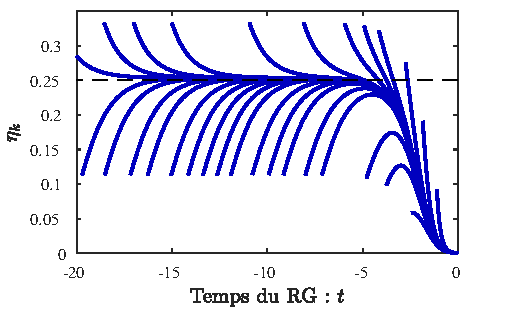
\includegraphics[width=0.95\columnwidth]{etakd2.pdf}
		\caption{Évolution de $eta_k$ en fonction de $t= \ln(k)$ pour différentes etapes de la dichotomie sur $r_0'$. En pointillé noir nous avons représenté la valeur exacte attendue $\eta = 0.25$. }
		\label{fig:etakd2}
	\end{center}
\end{figure}

La \refig{etakd2} montre l'évolution de $\eta_k$ pour plusieurs conditions initiales $r_0'$ et donc pour plusieurs étapes de la dichotomie du $r_0'$ nous menant vers un point critique. On remarque que pour des temps $t<-5$ nous avons des courbes passant par un plateau. Ce plateau correspond au point fixe pour lequel $\eta_k = \eta$ est une constante. Après être passées par ce plateau les courbes divergent (en partant soit vers le haut, soit vers le bas). Ceci s'explique par le fait que nous n'avons pas trouvé avec une précision infinie la valeur de $r_0'$ menant au point fixe. De ce fait n'étant pas parfaitement au point critique mais très proche on montre qu'effectivement les courbes passent par le plateau du point fixe mais en diverge en $\exp(-t/\nu)$ ou $\nu$ est l'exposant critique.

Nous trouvons donc ...\\



\subsection{Pour $N = 2$ ou 3, $d=2$}

Le cas $N = 2$ ou 3, $d=3$ fonctionnant nous nous sommes ensuite plus particulièrement intéressé au cas $N = 2$, $d = 2$. La première difficulté que nous avons rencontré lors de ces simulations a été la présence probable d'un pôle dans l'expression de $G_k(q, \rho)$ lorsque l'on 

Nous avons aussi fait varier le nombre de points d'intégration ou encore la taille de la grille de discrétisation en champ $\rho$. Cependant nous n'avons trouvé aucun changement de comportement des résultats.
Nous en avons déduit qu'il s'agissaient d'un problème de précisions sur les

\end{multicols}
\begin{figure}[H]
	\begin{center}
		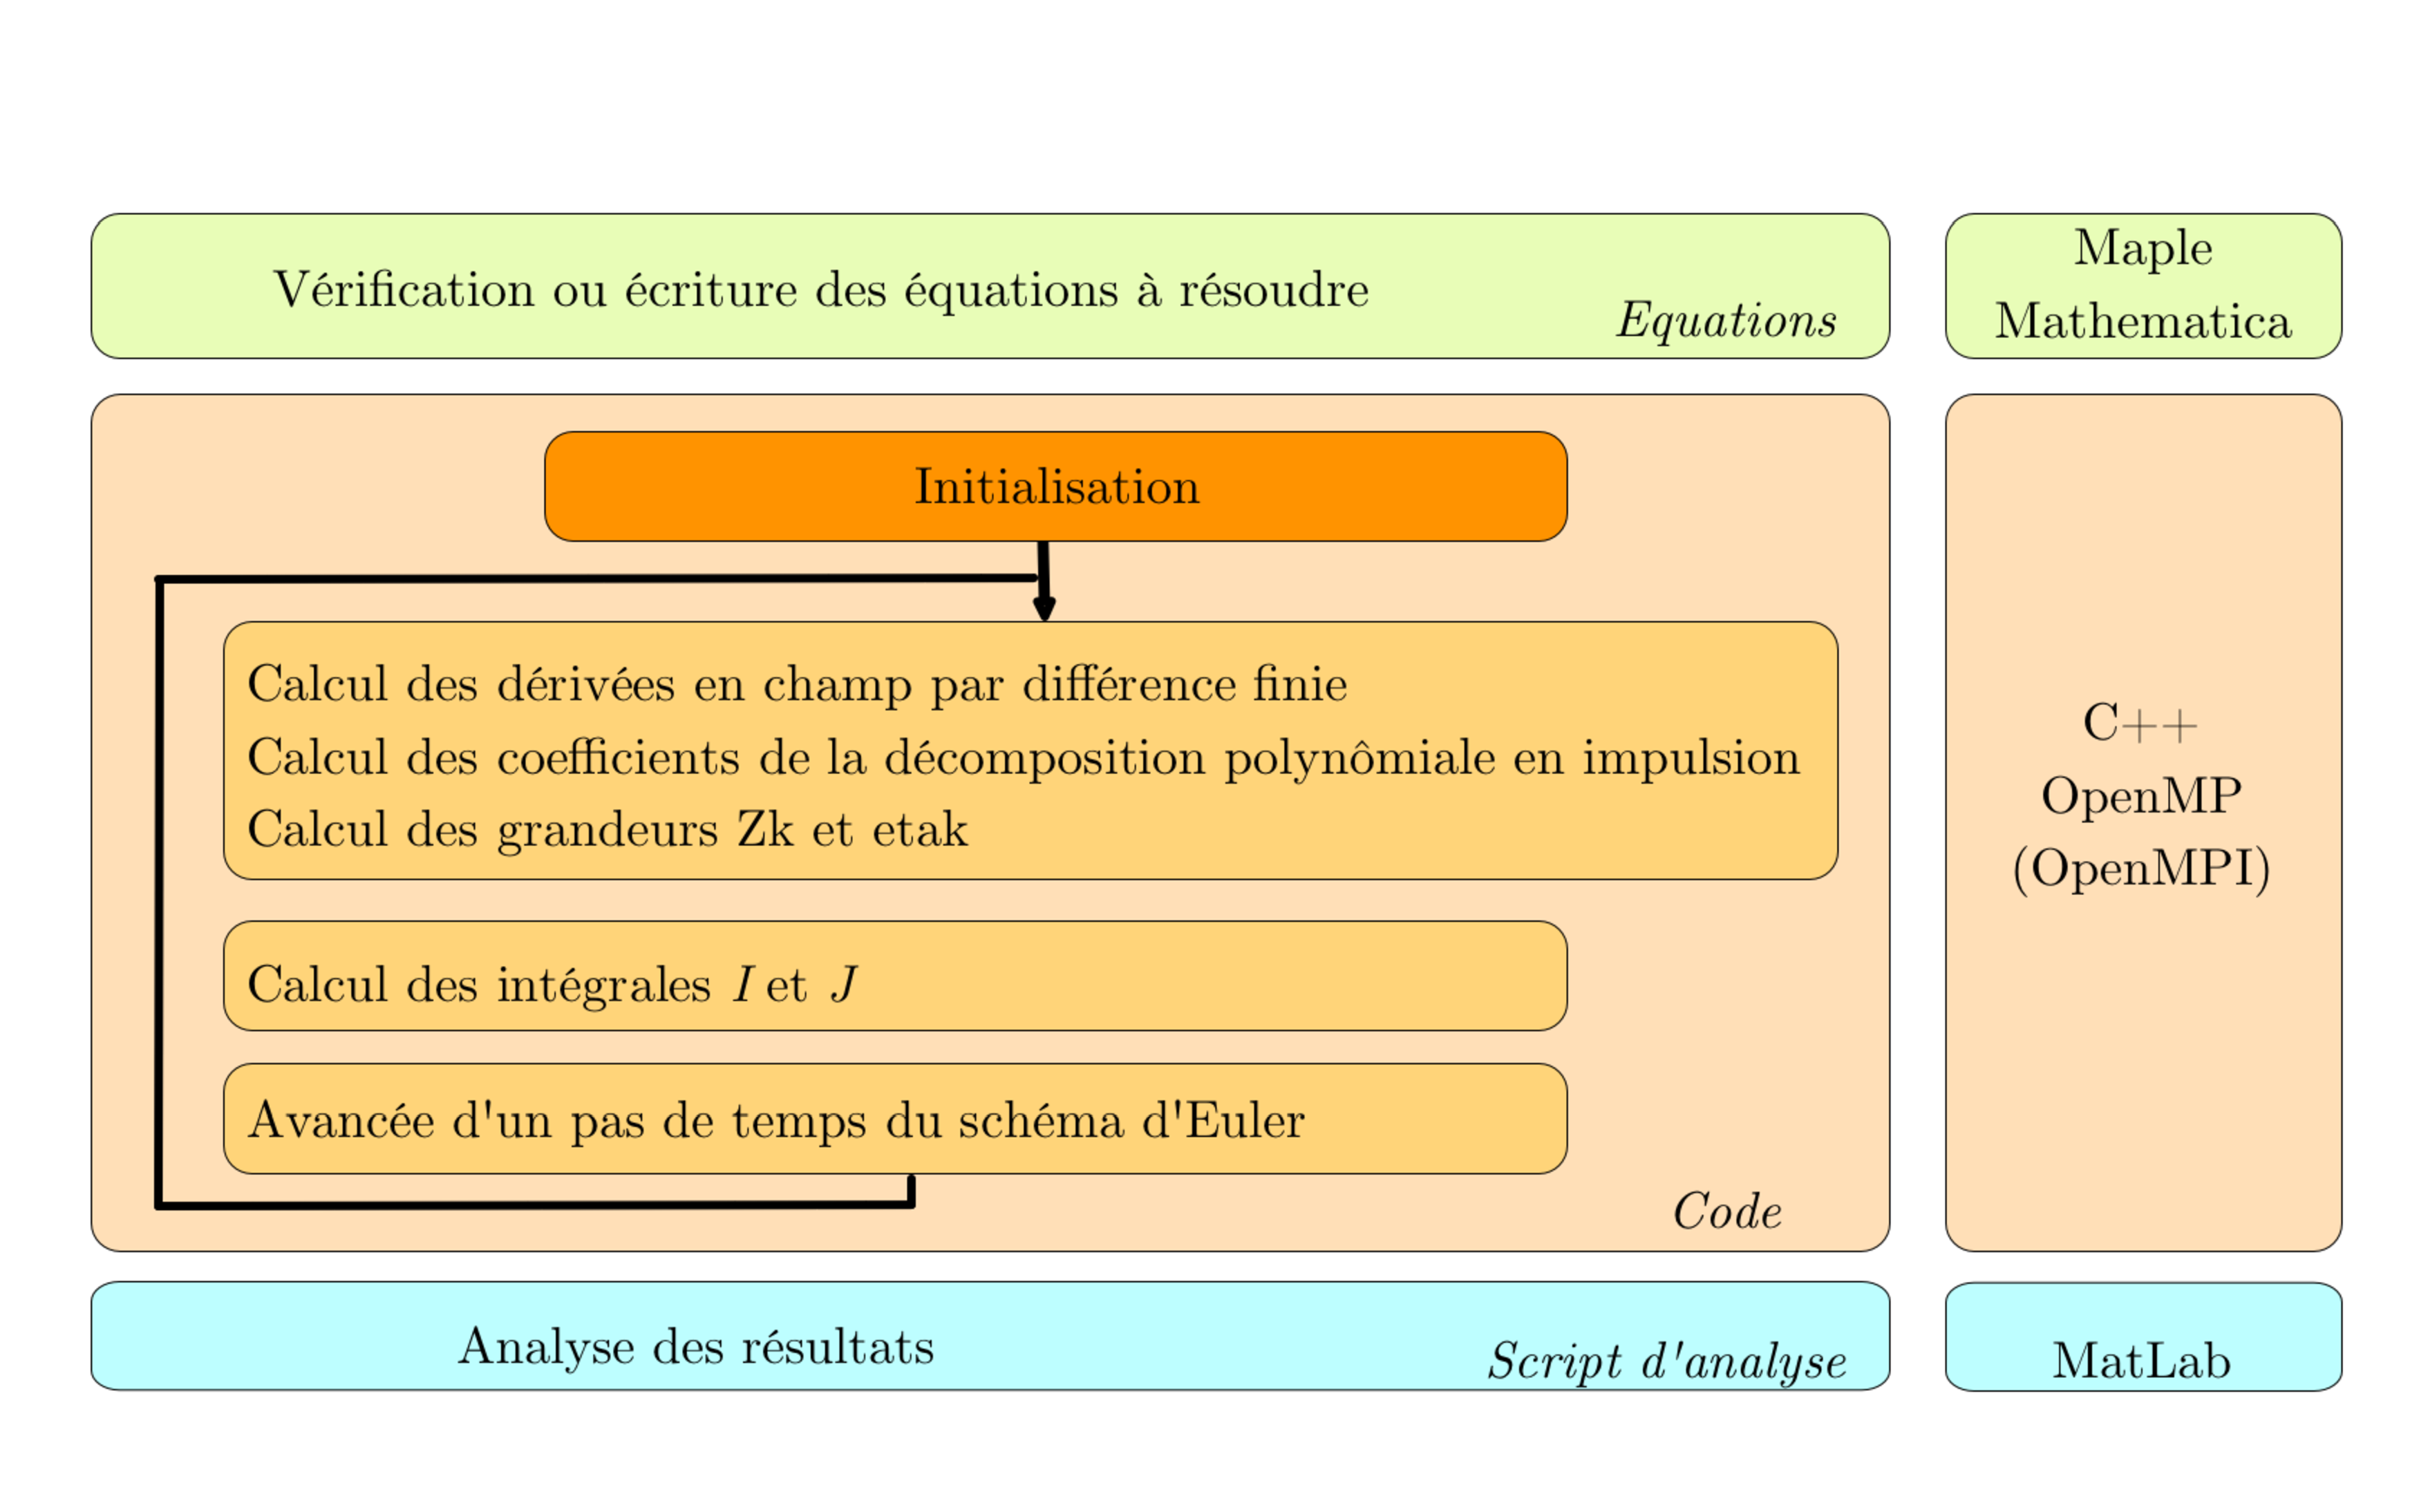
\includegraphics[width=0.95\columnwidth]{Diagramme_Code_2.pdf}
		\caption{Schéma de la répartition du travail effectué. Nous avons commencé par retrouver ou écrire les équations BMW à résoudre (vert). Ensuite nous avons réécrit ou écrit les codes C++ de simulation de ces équations ayant la structure indiquée (rouge). Toutes les parties orangées sont parallélisée sous OpenMP. Enfin nous étudions les résultats à l'aides de scripts Matlab.}
		\label{fig:org}
	\end{center}
\end{figure}

\begin{multicols}{2}


\newpage
\phantom{.}
\newpage


\section{Le modèle d'Ising en dimension 2}

\subsection{Présentation du modèle d'Ising}

\label{sec:IsingIntro}


On considère le modèle d'Ising classique sur un réseau hypercubique de dimension $d$ (nous avons uniquement travaillé numériquement dans le cas $d=2$ mais nous exposons le formalisme pour une dimension $d$ quelconque). Les longueurs sont exprimées en unité du pas du réseau. On note $\{\ev_\nu\}_{\nu\in\bbrac{1,d}}$ la base cartésienne associée. L'hamiltonien du système non excité, en contact seulement avec le milieu extérieur qui a une température fixe et dans lequel ne se trouve aucun champ magnétique, est donné par\footnote{Nous avions jusqu'à présent noté $H$ le hamiltonien du système total prenant en compte les excitations extérieures et $S$ celui du système non excité. Ici nous utilisons la notation $H$ pour le système non excité pour ne pas confondre hamiltonien et spin $S_\rv$.}
\begin{equation}
H = -J\beta \sum_{\left<\rv, \rv'\right>}S_\rv S_{\rv'}
\label{eq:HamIsing}
\end{equation}
Où $S_\rv \in \{-1,1\}$ représente la valeur du spin (i.e. sa direction selon l'axe $z$, c.f. \refig{schemaIsing}) à la position $\rv$. La notation $\left<\rv, \rv'\right>$ signifie que le terme $S_\rv S_{\rv'}$ contribue à la somme si et seulement si ce sont deux spins plus proches voisins du réseau (i.e s'il existe $\nu \in \bbrac{1,d}$ tel que $\rv' = \rv \pm \ev_\nu$). Le paramètre $J$ représentant une énergie est une constante positive. La variable $\beta = 1/(k_BT)$ où $k_B$ est la constante de Boltzmann représentant l'influence de la température $T$ à laquelle est soumis le système.
\setlength{\unitlength}{1cm}
\begin{figure}[H]
\begin{center}
\begin{picture}(6,3.8)

\put(-0.5,1){\vector(0,1){2}}
\put(-0.8,2){$z$}

\color{cyan}
\put(0,0){\line(1,3){1.2}}
\put(1,0){\line(1,3){1.2}}
\put(2,0){\line(1,3){1.2}}
\put(3,0){\line(1,3){1.2}}
\put(4,0){\line(1,3){1.2}}
\put(5,0){\line(1,3){1.2}}

\put(-0.25,0.45){\line(1,0){5.7}}
\put(0.05,1.25){\line(1,0){5.7}}
\put(0.25,2.0){\line(1,0){5.7}}
\put(0.45,2.70){\line(1,0){5.7}}
\put(0.65,3.35){\line(1,0){5.7}}
\color{red}
\linethickness{0.35mm}

\put(0.15,0.85){\vector(0,-1){0.8}}
\put(1.15,0.05){\vector(0,1){0.8}}
\put(2.15,0.85){\vector(0,-1){0.8}}
\put(3.15,0.05){\vector(0,1){0.8}}
\put(4.15,0.05){\vector(0,1){0.8}}
\put(5.15,0.85){\vector(0,-1){0.8}}

\put(0.4167,1.6){\vector(0,-1){0.7}}
\put(1.4167,0.9){\vector(0,1){0.7}}
\put(2.4167,0.9){\vector(0,1){0.7}}
\put(3.4167,0.9){\vector(0,1){0.7}}
\put(4.4167,1.6){\vector(0,-1){0.7}}
\put(5.4167,0.9){\vector(0,1){0.7}}

\put(0.667,1.7){\vector(0,1){0.6}}
\put(1.667,1.7){\vector(0,1){0.6}}
\put(2.667,2.3){\vector(0,-1){0.6}}
\put(3.667,1.7){\vector(0,1){0.6}}
\put(4.667,1.7){\vector(0,1){0.6}}
\put(5.667,1.7){\vector(0,1){0.6}}

\put(0.9,2.45){\vector(0,1){0.5}}
\put(1.9,2.95){\vector(0,-1){0.5}}
\put(2.9,2.45){\vector(0,1){0.5}}
\put(3.9,2.45){\vector(0,1){0.5}}
\put(4.9,2.95){\vector(0,-1){0.5}}
\put(5.9,2.45){\vector(0,1){0.5}}

\put(1.1167,3.55){\vector(0,-1){0.4}}
\put(2.1167,3.15){\vector(0,1){0.4}}
\put(3.1167,3.15){\vector(0,1){0.4}}
\put(4.1167,3.55){\vector(0,-1){0.4}}
\put(5.1167,3.55){\vector(0,-1){0.4}}
\put(6.1167,3.15){\vector(0,1){0.4}}

\end{picture}
\end{center}
\caption{Exemple de réseau d'Ising en dimension $d=2$. On traite dans le modèle d'Ising des spins avec une seule composante, ce sont donc des vecteurs dont seule la direction peut changer mais pas l'orientation qui est fixé ici selon $z$, perpendiculairement au plan). On décrit donc un spin à la position $\rv$ du plan (xy) par une valeur $1$ (quand il pointe vers le haut) ou $-1$ (vers le bas). Le système est dans la phase haute température ($T>T_c$) car les spins ont des directions aléatoire. Le nombre de spins représenté est faible, mais comme nous ferons une étude à la limite thermodynamique il est bien plus élevé dans le système étudié.}
	\label{fig:schemaIsing}
\end{figure}
Sur un tel système nous observons une transition de phase du second ordre. En effet il existe une phase (dite de symétrie brisée, ou encore basse température) dans laquelle les spins tendent tous à s'aligner dans une direction privilégiée lorsque la température et faible et que les fluctuations thermiques ne jouent pas un rôle important\footnote{En effet à température faible la configuration du système la plus stable et qui se produit expérimentalement est celle pour laquelle l'hamiltonien est minimal. Comme $J>0$ ceci se produit lorsque tous les $\S_\rv$ possède la même valeur, i.e.lorsque tous les spins sont alignés.}. Lorsque l'on dépasse la température critique $T_c$ l'énergie thermique que reçoit le système est suffisamment importante pour que les spins prennent une direction plus ou moins aléatoire le système est alors dans une nouvelle phase (dite symétrique). C'est ce modèle qui explique la perte d'aimantation d'un métal à haute température que nous avions mentionné dans l'introduction. \\


Si l'on change l'axe $z$ en $-z$ alors l'hamltonien du système ne change pas. Ainsi ce système possède une symétrie $O(1)$. Il est donc possible de calculer ces exposants critiques en utilisant les équations BMW de la \refsec{} développée avec l'hamiltonien la théorie $\varphiv^4$. La température critique n'étant pas une quantité universelle, elle dépend entièrement du système et prendre un hamiltonien tronqué ne suffit pas, la forme même du réseau est importante, la forme exacte du hamiltonien doit être prise en compte.

Or comme \refeq{HamIsing} ne correspond pas aux hamiltoniens dépendants d'un champ étudiés dans toute la première partie de cette étude, il ne semble donc pas possible a priori de lui appliquer le NPRG. En revanche il est tout de même possible de définir une nouvel hamiltonien exactement équivalent à $H$ en réécrivant avec des champ la fonction de partition du système à l'aide d'une transformée de Hubbard-Stratanovitch comme détaillé dans le paragraphe suivant. \\ 

La particularité de ce modèle est aussi qu'il a déjà été complètement résolu analytiquement par Onsager \cite{Onsager} en 1944. Tout est donc déjà connu et notamment la température critique de la transition de phase. Avec l'approche BMW nous avons essayé de la retrouver pour valider la qualité de l'approximation et la possibilité de calculer la température critique $T_c$ par les équations du NPRG. 

%\vspace*{11pt} 

\subsection{Modélisation avec des champs}

Pour des raisons pratiques on définit maintenant un hamiltonien légèrement modifié
\begin{align}
  H_\mu &= -J\beta \sum_{\left<\rv, \rv'\right>}S_\rv S_{\rv'} - \mu \beta N_S \\
  H_\mu  &= -J\beta \sum_{\left<\rv, \rv'\right>}S_\rv S_{\rv'} - \mu \beta \sum_\rv S_\rv^2 
\end{align}
Avec la notation sur la somme 
\begin{equation}
\sum_\rv \,\, \equiv \sum_{x_1=1}^{N_1}\sum_{x_2=1}^{N_1} ... \sum_{x_d=1}^{N_1} 
\end{equation}
Où $N_\nu$ est le nombre de spins dans la direction $\ev_\nu$, et $\rv \equiv (x_1, x_2, ..., x_d)$. Le nombre $N_S \equiv N_1N_1...N_d$ est le nombre total de spins. Physiquement, ajouter une constante à $H$ ne change rien car cela ne fait que décaler l'origine arbitraire des énergies. En revanche cela a un avantage mathématique. En effet, on pose $A_{\rv, \rv'}^{(\mu)}$ la matrice définie implicitement dans $\mathscr{M}_{N_S}(\R)$ par
\begin{equation}
  H_\mu  = -\frac{1}{2} \sum_{\rv, \rv'} S_\rv A_{\rv, \rv'}^{(\mu)}S_{\rv'}
\end{equation}

Il est alors possible de choisir $\mu$ suffisamment grand pour que $A_{\rv, \rv'}^{(\mu)}$ soit à diagonale strictement dominante et donc inversible. Il suffit de prendre $\mu > dJ$. \\

On peut alors réaliser une transformée de Hubbard-Stratanovitch. Pour cela commençons par écrire la fonction de partition du système modèle
\begin{equation}
  \Zc = \sum_{\{S_\rv\}} e^{-H_{\mu}} =\sum_{\{S_\rv\}}  \exp\(\frac{1}{2} \sum_{\rv, \rv'} S_\rv A_{\rv, \rv'}^{(\mu)}S_{\rv'}\)
\end{equation}
Par integration gaussienne \textit{inverse} il vient, 
\begin{equation}
\begin{split}
  \Zc & \propto \sum_{\{S_\rv\}} \int_\R \prod_{\rv} \, \dd \varphi_\rv \, e^{ -\frac{1}{2} \sum\limits_{\rv, \rv'} \varphi_\rv {(A_{\rv, \rv'}^{(\mu)})}^{-1} \varphi_{\rv'} +\sum\limits_\rv  \varphi_\rv S_\rv  } \\
  \Zc & \propto \int_\R \prod_{\rv} \, \dd \varphi_\rv \, e^{ -\frac{1}{2} \sum\limits_{\rv, \rv'} \varphi_\rv {(A_{\rv, \rv'}^{(\mu)})}^{-1} \varphi_{\rv'} + \sum\limits_\rv \ln\(\cosh(\varphi_\rv)\) } \\
\end{split}
\end{equation}

Cependant nous ne pouvons pas exprimer facilement ${(A_{\rv, \rv'}^{(\mu)})}^{-1}$. Pour cela il est pratique de réaliser une transformée de Fourier Semi-Discrète (TFSD - c.f. \refann{TFSD}) en posant, pour $\qv \in [-\pi, \pi]^d$,
\begin{equation}
  {\varphi}(\qv) = \sum_\rv \varphi_\rv e^{-i\qv\rv} \quad \text{et} \quad \varphi_\rv = \int_\qv {\varphi}(\qv)  e^{i\qv\rv}
\end{equation}
En effet comme expliqué ci-après, ${(A^{(\mu)})}^{-1}$ est " diagonal" en TFSD. Montrons le en commençant par poser $K_\mu$ l'expression
\begin{equation}
	K_\mu = \sum\limits_{\rv, \rv'} \varphi_\rv {(A_{\rv, \rv'}^{(\mu)})} \varphi_{\rv'}
\end{equation} 
En utilisant la définition implicite de ${(A_{\rv, \rv'}^{(\mu)})}$ et en passant en TFSD nous obtenons
\begin{equation}
\begin{split}
  K_\mu = -J\beta & \sum_{\left<\rv, \rv'\right>} \iint_{\qv,\qv'} {\varphi}(\qv) {\varphi}(\qv')  e^{i(\qv\rv+\qv'\rv')} \\
   -\mu\beta & \sum_\rv \iint_{\qv,\qv'} {\varphi}(\qv) {\varphi}(\qv')  e^{i(\qv+\qv')\rv}
\end{split}
\end{equation}
\commentout{
\begin{equation}
\begin{split}
  K_\mu = -J\beta & \sum_{\rv}\sum_{\nu}   \iint_{\qv,\qv'} {\varphi}(\qv) {\varphi}(\qv')  e^{i((\qv+\qv')\rv \pm \qv'\ev_\nu)} \\
   -\mu\beta & \sum_\rv \iint_{\qv,\qv'} {\varphi}(\qv) {\varphi}(\qv')  e^{i(\qv+\qv')\rv}
\end{split}
\end{equation}
\begin{equation}
\begin{split}
  K_\mu = -J\beta & \iint_{\qv,\qv'} {\varphi}(\qv) {\varphi}(\qv')  \sum_{\rv}  e^{i(\qv+\qv')\rv} \sum_{\nu} e^{ \pm i \qv'\ev_\nu}  \\
   -\mu\beta & \sum_\rv \iint_{\qv,\qv'} {\varphi}(\qv) {\varphi}(\qv')  e^{i(\qv+\qv')\rv}
\end{split}
\end{equation}
}
Notons donc simplement
\begin{equation}
  \lambda_\mu(\qv) = -\beta \left\{ J\sum_{\nu} e^{ \pm i \qv \, \ev_\nu} +\mu \right\} 
\end{equation}
Ainsi, il vient, 
\begin{equation}
  K_\mu =   \iint_{\qv,\qv'} {\varphi}(\qv) {\varphi}(\qv')   \lambda_\mu(\qv')   \sum_{\rv}  e^{i(\qv+\qv')\rv} \\
\end{equation}
\begin{equation}
  K_\mu =   \iint_{\qv,\qv'} {\varphi}(\qv) {\varphi}(\qv')   \lambda_\mu(\qv')   D_{N_S}(\qv+\qv') \\
\end{equation}
En définissant le noyaux de Dirichlet $D_{N_S}$ par
\begin{equation}
  \forall \pv \in [-\pi, \pi]^d \quad D_{N_S} (\pv) =  \sum_{\rv} e^{i \pv \rv} 
\end{equation}
\commentout{
\begin{equation}
  \begin{split}
  \sum_{x=0}^{N_x} e^{ix(\qv+\qv')_x }  = \frac{1 - e^{i(N_x+1)(\qv+\qv')_x}}{1-e^{i(\qv+\qv')_x }} \\
  = \frac{\sin{\(  \frac{(N_x+1)}{2}(\qv+\qv')_x \)}}{\sin{\( \frac{1}{2}(\qv+\qv')_x \) }} e^{i\frac{N_x}{2}(\qv+\qv')_x }
\end{split}
\end{equation}}

\commentout{
On note $\Dc = \Dc([-\pi, \pi]^2)$, soit $f \in \mathcal{D}$, $D_{N_S}$ étant une fonction de $L^2([-\pi, \pi]^2)$, il appartient à $\Dc'$. On montre alors que \cite{}
\begin{equation}
  \lim\limits_{N_S \rightarrow +\infty} \left< D_{N_S} , f \right>_{\Dc', \Dc} =  \left< \delta , f \right>_{\Dc', \Dc}
\end{equation}
}

Ainsi, en prenant la limite $N_S \rightarrow + \infty$ et en raisonnant au sens des distributions, par les propriétés du noyau de Dirichlet, il vient formellement
\begin{equation}
 \lim_{N_S \rightarrow + \infty} K_\mu = - \int_\qv {\varphi}(\qv)  \lambda_\mu(\qv) {\varphi}(-\qv)
\end{equation}
Dans la suite nous ferons l'hypothèse de la limite thermodynamique, selon laquelle $N_S$ est suffisamment grand pour que l'on écrive, par abus de notation, $K_\mu = \lim\limits_{N_S \rightarrow + \infty} K_\mu$. \\
Nous obtenons alors
\begin{equation}
  K_\mu = - \int_\qv {\varphi}(\qv)  \lambda_{\mu}(\qv) {\varphi}(-\qv)
\end{equation}
Et on en déduit la transformée de Fourier de $A_{\rv, \rv'}^{(\mu)}$
\begin{align}
  {A}(\qv, \qv') = 
  \begin{cases}
    \lambda_{\mu}(\qv) \quad  & \text{si } \qv' = - \qv\\
    0 \quad & \text{si } \qv' \neq - \qv
  \end{cases}
\end{align}
Autrement dit, $A^{(\mu)}$ est un opérateur diagonal et bien inversible si $\mu > Jd$. Notons,
\begin{equation}
	\gamma(\qv ) = \frac{1}{d} \sum\limits_{\nu=1}^{d} \cos(q_\nu)
\end{equation}
L'expression de $\lambda_\mu$ se trouve alors être 
\begin{equation}
	 \lambda_\mu(\qv) = 2\beta\(J d \gamma(\qv) + \mu\)
\end{equation}
Par les propriétés de la TFSD il vient,
\begin{equation}
  \Zc  \propto \int_\R \prod_{\rv} \, \dd \varphi_\rv \, e^{-S_\mu[\varphi] } \, ,
\end{equation}
avec l'hamiltonien $S_\mu$ s'écrivant :
\begin{equation}
  S_\mu[\varphi] = \frac{1}{2} \int_\qv \varphi(\qv) \frac{1}{\lambda_\mu(\qv)} \varphi(-\qv) - \sum\limits_\rv \ln\(\cosh(\varphi_\rv)\)
\end{equation}
Par isometrie de la transformation de Fourier, et donc par le théorème de Parseval, nous réecrivons $S_\mu$ sous la forme 
\begin{equation}
  \begin{split}
    S_\mu[\varphi] & = \frac{1}{2} \int_\qv \varphi(\qv) \[\frac{1}{\lambda_\mu(\qv)} - \frac{1}{\lambda_\mu(0)}\] \varphi(-\qv) \\
    &+ \sum\limits_\rv \[\frac{1}{2\lambda_\mu(0)}\varphi_\rv^2 - \ln\(\cosh(\varphi_\rv)\) \]
  \end{split}
\end{equation}
Enfin, soit $\delta \in \R^+_*$, on pose le changement de variable, 
\begin{equation}
  \varphi \rightarrow \delta\sqrt{2 \beta J d} \, \varphi 
\end{equation}
On obtient alors 
\begin{equation}
S_\mu[\varphi] = \frac{1}{2} \int_\qv {\varphi}(\qv)\eo(\qv){\varphi}(-\qv) + \sum_\rv U(\varphi(\rv))
\end{equation}
Avec, en posant $\tilde{\mu} = \mu/(Jd)$ et $\tilde{\beta} = \beta Jd$,
\begin{equation}
  \eo(\qv) = \delta^2\frac{1 - \gamma(\qv)}{(\gamma(\qv) + \tilde{\mu})(1+\tilde{\mu})}
\end{equation}
\begin{equation}
  U(\phi) = \delta^2 \frac{1}{1+\tilde{\mu}} \frac{1}{2}\phi^2 - \ln\(\cosh\(\delta\sqrt{2\tilde{\beta}}\phi\)\)
\end{equation}

On se retrouve donc ici avec la formulation d'un problème de théorie des champs que l'on peut résoudre avec le NPRG et notamment avec l'approximation BMW. Le nouvel hamiltonien $S_\mu$ est complètement équivalent à $H_\mu$ donc il permet d'en récupérer exactement toutes les informations physiques. Concernant la mise en pratique du NPRG, la seule différence avec tout ce qui a été étudié précédemment c'est qu'ici, par TFSD les intégrales sur les impulsions ne sont plus calculées sur un domaine infini mais sur "la première zone de Brillouin", i.e. sur l'hypercube $[-\pi, \pi]^d$. L'équation de flot BMW \refeq{flotBMW} reste valable en prenant en compte cet ajustement.\\

La fonction $U$ représente alors le potentiel du système dans l'approximation de champ moyen. Et ainsi le potentiel $V_k$ des équations BMW prend en $k=\Lambda$ la valeur $V_\Lambda = U$. La fonction $\eo$ s'appelle quant à elle la relation de dispersion. Dans le modèle continu $\varphiv^4$ il y avait de même une relation de dispersion qui valait alors $\varepsilon(\pv) = \pv^2$.\\
 
 
Remarquons de plus que la fonction $U$ est de classe $\Cc^\infty$ dérivable sur $[0,+\infty[$, avec
\begin{equation}
\partial_\phi^2 U(\phi) = \delta^2 \frac{1}{1+\tilde{\mu}} - \frac{2\delta^2\tilde{\beta} }{\cosh^2\(\delta\sqrt{2\tilde{\beta}}\phi\)} 
\label{eq:derU}
\end{equation}

Enfin, la recherche de point fixe pour se système se fait en variant le paramètre $\tilde{\beta}$. On cherche donc $\tilde{\beta}_c = Jd/(k_BT_c)$ pour lequel les équations dimensionnées écrites plus loin possède un point fixe. De cette manière on obtient la température critique.

\commentout{
Ceci nous permet de récupérer la valeur que l'on aurait trouvé en calculant la température critique $\tilde{T}_c^{\text{MF}} = T_c^{\text{MF}}/(Jd) $ en s'appuyant sur une théorie de champ moyen. En effet, dans une théorie de champ moyen le potentiel du système est directement le potentiel $U$. Or on rappelle que la phase dans laquelle on se trouve dépend du potentiel, de la position de son minimum et de sa forme de manière générale. Nous savons qu'en dessous de la température critique $U$ est une fonction concave au voisinage de $\phi = 0$ et au dessus c'est une fonction convexe. Ainsi, à la transition $X(0) = 0$. Ceci nous donne

\begin{equation}
 \frac{1}{\tilde{T}_c^{\text{MF}}} = \tilde{\beta}_c^{\text{MF}} \simeq \frac{1}{2(1+\tilde{\mu})}
\end{equation}

Cette valeur nous donne déjà une borne supérieure sur la température critique que l'on recherche. En effet, on sait que la vraie température critique sera toujours plus faible que celle obtenue par approximation de champ moyen\footnote{Ceci s'explique en partie "avec les mains". En effet dans une approximation de champ moyen, comme son nom l'indique les fluctuations des degrés de libertés - ici l'orientation des spins - autour s'une position moyenne se trouvent être négligées. Or leur prise en compte pour la résolution complète du modèle implique que pour une même température le système complet est plus désordonné que ce que le calcul champ moyen nous donne. La température critique vraie sera donc plus basse que la température critique champ moyen} : $T_c < T_c^{\text{MF}}$.
}


\subsection{Régulateur}

Dans le but de réécrire les équations BMW pour le hamiltonien que nous avons précédemment nous exprimons le nouveau régulateur à utiliser du à la présence d'une nouvelle relation de dispersion $\eo$. Pour satisfaire toues les conditions d'un régulateur on utilise ici
\begin{equation}
	\Rc_k(\qv) = \alpha \frac{Z_k \eo(\qv)}{\exp{(\eo(\qv)/\varepsilon_k)} -1}
\end{equation}
Avec $\varepsilon_k = \| \eo \|_\infty k^2$. Les expressions de $\partial_t \Rc_k$ se trouvent en \refann{Ising2D}. Notons aussi que dans certaines équations que nous avons utilisées le facteur $Z_k$ a pu être omis car il ne sert qu'à avoir des dimensions compatibles lors de l'adimensionnement des équations. 

\begin{figure}[H]
\begin{center}
	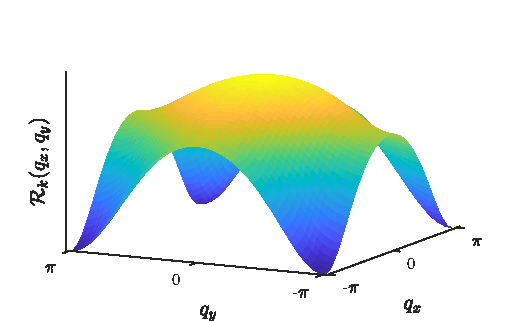
\includegraphics[width=0.8\columnwidth]{RegIsing.pdf}
\end{center}
\caption{Allure du régulateur choisi pour une valeur de $k\simeq 1$ dans la dimension étudié $d=2$.}
\end{figure}



\subsection{Étapes de la résolution}

Pour des raisons pratiques nous avons décomposé la résolution numérique des équations BMW du modèle d'Ising en 3 étapes, en procédant à un adimensionnement progressif des équations. \\

On commence par réécrire \refeq{gammaDecomp} adaptée avec la relation de dispersion $\eo$ selon
\begin{equation}
\Gamma^{(2)}(\pv, \phiv) = \eo(\pv) + \Delta_k(\pv, \phi) + X_k(\phi)
\label{eq:decompBMWIsing2D}
\end{equation} 
où l'on introduit $X_k(\phi) = \partial_{\phi}^2 V_k(\phi)$.
Cette nouvelle écriture insérée dans \refeq{flotBMW} donne alors les trois jeux d'équations BMW pour le système Ising 2D auquel il faut ajouter les conditions initiales comme détaillé ci-après.


\subsubsection{Première étape}

Comme nous travaillons sur un réseau, les fonctions que l'on considère sont $2\pi$ périodiques selon les composantes des impulsions lorsque l'on considère les variables et les fonctions dimensionnées (c.f. \refsec{RG}). (i.e. les fonctions et variables notées de manière générale sans tilde). Ceci permet de s'affranchir de certaines approximations numériques dans le calcul des intégrales. Il est donc préférable de commencer par résoudre le système d'équation BMW brut, noté $\Ec_1$, sans réaliser d'adimensionnement (directement obtenu de \refeq{flotBMW}) pour $k $ variant de $\Lambda$ à $k_a$ (où $k_a \in ]0, 1]$ a une valeur déterminée). Le problème BMW ($\Pc_1$) à résoudre est donc \\

\noindent
{\itshape Trouver $\Delta_k$, $X_k$, solution de $\Ec_1$, i.e tels que pour tout $p_x \in [-\pi, \pi]$, $p_y \in [-\pi, \pi]$, $\phi \in \R$, $k\in [k_a, \Lambda]$}


\begin{align}
	\partial_t  \Delta_k (p_x, p_y, \phi) & = 
	\begin{aligned}[t]
	&  J_3(p_x, p_y, \phi) \partial_{\phi} \left\{ \Delta_k (p_x, p_y, \phi) + X_k(\phi) \right\} \\
	&  - \frac{1}{2} I_2(\phi) \partial_{\phi}^2 \Delta_k(p_x, p_y, \phi) \\
	& - I_3(\phi){(\partial_{\phi} X_k(\phi))}^2
	\end{aligned}
	\label{eqn} \\
	\partial_t X_k(\phi) & = 
	\begin{aligned}[t]
		& \frac{1}{2} \partial_{\phi}^2 I_1(\phi)
	\end{aligned}
\end{align}



Où l'on note toujours $X_k(\phi) = \partial_{\phi}^2 V_k(\phi)$. Ce système est similaire au système (\refeq{sysDeltaON1}, \refeq{sysDeltaON2}) du modèle $\varphiv^4$ mais il est écrit selon la variable $\phi$ et les fonctions dépendent non plus de la norme des impulsions mais bien des deux composantes de $\pv$, que sont $p_x$ et $p_y$ en dimension $d=2$. Les notations $J$ et $I$ correspondent à celle du modèle $\varphiv^4$ et leurs expressions sont écrites en \refann{Ising2D}. \\


Les conditions initiales de ce problème viennent de la décomposition \refeq{decompBMWIsing2D}, ainsi que de la condition initiale générale des équations BMW \refeq{initFlotBMW} associé à l'expression de la dérivée seconde de $U$ par rapport à $\phi$, \refeq{derU}
\begin{equation}
	\Delta_\Lambda = 0 \quad \text{et} \quad X_\Lambda(\phi) =  \delta^2 \frac{1}{1+\tilde{\mu}} - \frac{2\delta^2\tilde{\beta} }{\cosh^2\(\delta\sqrt{2\tilde{\beta}}\phi\)}
\end{equation}

\vspace*{11pt}

\subsubsection{Deuxième étape}


Dans un second temps pour $k \in [k_b, k_a]$ (où $ 0 < k_b < k_a < 1$) on utilise un nouveau système équations $\Ec_2$ pour lesquelles nous avons adimensionné les impulsions. En fait ceci correspond seulement à écrire les équations en fonction de $\tilde{\pv} = \pv/k$ (ou $\tqv = \qv/k$) au lieu de $\pv$ (ou $\qv$). Ces nouvelles équations prennent pour conditions initiales le résultats de la résolution numérique de $\Ec_1$ en $k = k_a$. Cela permet d'améliorer la précision du calcul des intégrales à $k$ petit (i.e. $k < k_a < 1$), même si, en contrepartie, on perd l'avantage de la périodicité des fonctions. \\
\indent
En effet pour un $k$ suffisamment faible la fonction $(k,\qv) \to \partial_t \Rc_k(\qv)$ possède une valeur non négligeable seulement pour des valeurs de $q_x$ et $q_y$ inférieures (voire très inférieure) à $\pi$ en valeur absolue. Or cette fonction apparait dans toutes les expressions des intégrales $I_n$ et $J_n$ de $\Ec_1$ qui sont calculées sur le carré $[-\pi, \pi]^2$ : 
\begin{equation}
	I_n, J_n \propto \int_\qv \partial_t \Rc_k(\qv)\times ... 
\end{equation}
Elle limite donc la zone utile d'intégration aux zones où elle n'est pas "quasi-nulle" (c.f. \refig{DerRegIsing}). Ainsi pour $k$ décroissant l'intervalle d'intégration réellement utile (qui contient l'information) diminue, il se concentre dans un cercle autour de l'origine. Ceci pose des problèmes de précision dans le calcul des intégrales quand on travaille avec un nombre de point de quadrature fixé. Autrement dit, l'échelle d'intégration ne correspond plus à l'échelle de variation des fonctions à intégrer. Seuls les points d'intégration présents dans la zone où $\Rc_k(\qv)$ possède une valeur non négligeable (zone jaune orange de \refig{DerRegIsing}) et apportent une contribution à l'intégrale. \\
\indent
L'adimensionnement $\tilde{\pv} = \pv/k$ permet d'éviter ce problème : il est équivalent à construire une boite numérique de discrétisation en impulsion \textit{dynamique}, (i.e. dont les dimensions diminuent au fur et à mesure que $k$ diminue vers $0$ dans la résolution) sans modifier le nombre de points de discrétisation. 
En effet, la nouvelle boite de discrétisation en $\tpv$ est définie par $[-\tp_{max}, \tp_{max}]^2$ ce qui correspondrait, pour la variable $\pv= k\tpv$, à une boite de dimension $[-k\tp_{max}, k\tp_{max}]^2 \subset [-\pi, \pi]^2$, diminuant avec $k$.


On peut choisir $k_a$ de manière à ce que $(k,\tqv) \to \partial_t \Rc_k(k\tqv)$ ne soit quasi-nulle que sur les bords de cette nouvelle boite en $\tqv$ pour tout $k \le k_a$ et que tous les points d'intégration servent. On conserve ainsi une précision de calcul constante à faible $k$. Le problème ($\Pc_2$) à résoudre devient \\


\noindent
{\itshape Trouver $\bDelta_k$, $\bX_k$, solution de $\Ec_2$, i.e tels que pour tout $\tp_x \in [-\tp_{max}, \tp_{max}]$, $\tp_y \in [-\tp_{max}, \tp_{max}]$, $\phi \in \R$, $k\in [k_b, k_a]$}

\begin{align}
	\partial_t  \bDelta_k (\tp_x, \tp_y, \phi) & = 
	\begin{aligned}[t]
	&  \bJ_3(\tp_x, \tp_y, \phi) \partial_{\phi} \left\{ \bDelta_k (\tp_x, \tp_y, \phi) + \bX_k(\phi) \right\} \\
	&  - \frac{1}{2} \bI_2(\phi) \partial_{\phi}^2 \bDelta_k(\tp_x, \tp_y, \phi) \\
	& - \bI_3(\phi){(\partial_{\phi} \bX_k(\phi))}^2 \\
	& + \tp_x \partial_{\tp_x} \bDelta_k (\tp_x, \tp_y, \phi)  \\
	& + \tp_y \partial_{\tp_y}  \bDelta_k (\tp_x, \tp_y, \phi) 
	\end{aligned}
	\label{eqn} \\
	\partial_t \bX_k(\phi) & = 
	\begin{aligned}[t]
		& \frac{1}{2} \partial_{\phi}^2 \bI_1(\phi)
	\end{aligned}
\end{align}
On pourra se référer à \refann{Ising2D} pour les différentes notations. Les conditions de raccordement sont
\begin{equation*}
\bDelta_{k_a}(\tp_x, \tp_y, \phi) = \Delta_{k_a}(p_x, p_y, \phi) \quad \text{et} \quad \bX_{k_a}(\phi) = X_{k_a}(\phi)
\end{equation*}

Pour assurer la compatibilité entre les deux systèmes il faut alors respecter $k_a\tp_{max} = \pi$. \\

\begin{figure}[H]
\begin{center}
	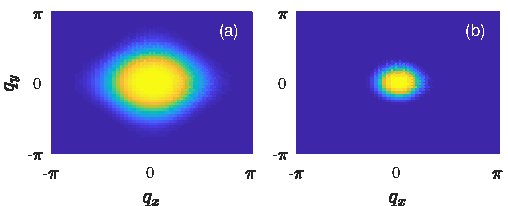
\includegraphics[width=0.95\columnwidth]{DerRegIsing.pdf}
	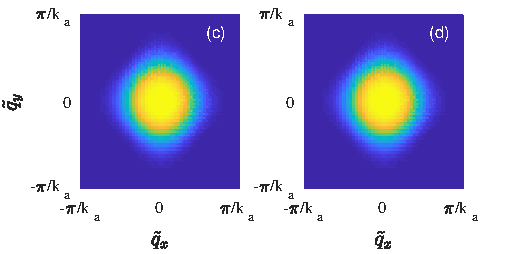
\includegraphics[width=0.95\columnwidth, height = 0.4\columnwidth]{DerRegIsing2.pdf}
\end{center}
\caption{(a-b) Représentation  de $(k, q_x, q_y) \to \partial_t \Rc_k(q_x, q_y)$ pour deux valeurs de  $k$ notées $k_1$ (a) et $k_2$ (b) sur la boite/carré de discrétisation en impulsion $[-\pi, \pi]^2$. Nous avons choisi $k1>k2$. On représente en fait la zone utile d'intégration dans $[\pi, \pi]^2$. En effet plus la couleur est bleue foncée plus la fonction est proche de 0. Ainsi on peut considérer que seule la partie dans la tache jaune contribue réellement à la valeur des intégrales, ailleurs la fonction est "quasi-nulle". (c-d) Représentation de $(k, \tq_x, \tq_y) \to \partial_t \Rc_k(k\tq_x, k\tq_y)$ dans la boite $[-\pi/k_a, \pi/k_a]^2$ pour  $k_1$ (c) et $k_2$ (d) en ayant choisi ici $k_a = k_1$. Il n'y a plus d'évolution de la zone utile d'intégration avec les nouvelles variables adimensionnée $\tq_x$ et $\tq_y$.}
\label{fig:DerRegIsing}
\end{figure}


\subsubsection{Troisième étape}

Enfin les deux jeux d'équation précédents utilise encore $\phi$ qui est dimensionné comme le sont resté les fonctions. Seules les variables d'impulsion $\pv$ et $\qv$ ont été changées pour des raisons pratiques. Or comme mentionné à plusieurs reprises, ce qui nous intéresse serait de trouver un point fixe du RG. En effet le but est de trouver la température critique du modèle d'Ising 2D et il faut, pour cela, essayer de se rapprocher d'un point fixe. On utilise alors, dans un dernier temps, un nouveau système $\Ec_3$ des équations totalement adimensionnées. On prend comme condition initiale le résultat donné par la simulation de $\Ec_2$ à $k = k_b$. Le problème se transforme alors en ($\Pc_3$), \\

\noindent
{\itshape Trouver $\tY_k$, $\tX_k$, solution de $\Ec_3$, i.e tels que pour tout $\tp_x \in [-\tp_{max}, \tp_{max}]$, $\tp_y \in [-\tp_{max}, \tp_{max}]$, $\tphi \in \R$, $k\in ]0, k_b]$}

\begin{equation}
\begin{split}
\partial_t & \tY_k(\tp_x, \tp_y,\tphi)  = \eta_k(1+\tY_k(\tp_x, \tp_y,\tphi)) \\
& + \frac{1}{2} \eta_k \tphi \partial_{\tphi} \tY_k(\tp_x, \tp_y,\tphi) - \frac{1}{2} \tI_2(\tphi) \partial_{\tphi}^2 \tY_k(\tp_x, \tp_y, \tphi) \\
&  + \frac{1}{\eo^0\tpv^2}\left\{ {\( \eo^0\tpv^2 \partial_{\tphi} \tY_k(\tp_x, \tp_y,\tphi) + \partial_{\tphi} \tX_k(\tphi)\)}^2 \tJ_3(\tp_x, \tp_y,\tphi) \right.\\
& \left. - {\( \partial_{\tphi} \tX_k(\tphi) \)}^2 \tI_3(\tphi)\right\} \\
& + \tp_x \partial_{\tp_x} \tY_k(\tp_x, \tp_y,\tphi) + \tp_y \partial_{\tp_y} \tY_k(\tp_x, \tp_y,\tphi) 
\end{split}
\end{equation}
\begin{equation}
\partial_t \tX_k(\tphi)  = (\eta_k -2)\tX_k(\tphi) + \frac{1}{2}\eta_k\tphi \, \partial_{\tphi}\tX(\tphi) + \frac{1}{2} \partial_{\tphi}^2 \tI_1(\tphi)
\end{equation}
On pourra ici aussi se référer à \refann{Ising2D} pour les différentes notations et plus de précision. Les conditions de raccordement sont
\begin{equation*}
\tY_{k_b}(\tp_x, \tp_y,\tphi) = \frac{1}{Z_k}\( 1+ \frac{\bDelta_{k_b}(\tp_x, \tp_y, \phi)}{\eo^0 k_b^2(\tp_x^2 +\tp_y^2)}\) -1
\end{equation*}
\begin{equation*}
\tX_{k_b}(\tphi) = \bX_{k_b}(\phi)
\end{equation*}
Avec une relation supplémentaire sur $\eta_k$
\begin{equation}
\eta_k = \frac{1}{2} \tI_2(0) \partial_{\tphi}^2 \tY_k(0,0,0) 
\end{equation}

En conclusion ici l'important est cette résolution numérique des équations que l'on découpe en trois parties distinctes pour utiliser au mieux la périodicité du problème. Ici encore, comme dans le modèle $\varphiv^4$ nos équations ne possèdent pas de conditions aux bords, seulement des conditions initiales.

\vspace*{11pt}

\section{Méthodes et outils numériques pour la résolution d'Ising 2D}

Nous allons passé en revu et justifié ici les principales méthodes numériques que nous avons utilisé pour tenter de résoudre les équations. En grande partie nous avons repris ce qui avait déjà été fait pour la résolution du modèle $O(N)$ en les adaptant à ces nouvelles équations.


\subsection{Structure du code}

La grosse différence entre les équations du modèle continu $\varphiv^4$ et ces nouvelles équations est qu'ici pour les dimensions d'impulsion les fonctions ne dépendent plus seulement de $p$ (i.e. la norme de $\pv$) mais de ces deux composantes $p_x$ et $p_y$. Ainsi nous avons conservé le choix de réaliser des intégrations avec la méthode de Gauss-Legendre tout en discrétisant les variables d'impulsion avec une méthode pseudo-spectrale de Tchebytchev pour des raisons détaillées dans les prochaines sections. La difficulté à alors résulté en la réécriture des méthodes à une dimension (i.e. pour des fonctions d'une variable en impulsion) déjà utilisées dans le modèle $ \varphiv^4$ en des méthodes à deux dimensions, pour des fonctions de deux variables d'impulsion. Le plus gros défit de ce code est encore de calculer les intégrales $J, \bJ, \tJ$. \\

Concernant la discrétisation en champ nous avons privilégié la variable $\phi$ dans les équations et non pas $\rho$ à causes de différents problèmes numériques mais nous sommes resté sur une discrétisation par une grille fixe et des calculs de dérivées par rapport à $\phi$ des fonctions inconnues à l'aide de schémas à 5 points. \\


Enfin, pour la discrétisation en temps $t$ le plus simple a été de conserver un schéma d'Euler explicite à cause de la non-linéarité des équations. Nous n'avons pas utilisé de schéma de Rung-Kutta car de manière générale le schéma d'Euler s'est avéré efficace.\\

Ce nouveau code est donc structuré de la même manière que le code du modèle continu $\varphiv^4$. En effet, avoir réécrit le code de la simulation du modèle continu $\varphiv^4$ en C++ de façon modulable à l'aide de classes nous a alors permis, de manière générale, de reprendre ou d'adapter beaucoup des fonctions numériques. Pour avoir une vue générale de la structure il est donc possible de se reporter encore à la figure \refig{org}. Nous détaillons, maintenant, ci-après les problèmes que l'on a pu rencontrer dans l'écriture des codes de simulations ainsi que les techniques retenues qui ont fonctionnées et leurs avantages comparés à celles qui ont échouées. 





\subsection{Problèmes rencontrés}

\label{sec:Problemes}

Tout d'abord nous avions écrit les équations en utilisant la variable $\rho$ pour résoudre $(\Pc_1)$. Cependant nous avons pu observer des instabilités dans le calcul des dérivées en $\rho$ pour $\rho = \rho_{max}$ (avec $\rho_{max}$ la limite de la grille de discrétisation en $\rho$). Nous avons réussi à résoudre le problème en descendant en ordre dans les schémas de calcul des dérivées en passant d'un ordre 5 à l'ordre 3. Cependant nous avons ensuite eu des instabilités au niveau du calcul des dérives $\partial_{\rho}$ autour de $\rho = 0$. Pour régler le problème nous avons alors utilisé la variable $\phi$. En effet il apparait alors des propriétés de parité des fonctions qui nous ont permis de donner des valeurs exactes aux dérivées en $\phi = 0$ (i.e. $\rho = 0$) et résoudre le problème. En outre la variable $\phi$ nous a aussi permis de repasser avec des dérivées en champs à 5 points sans difficultées. \\

Le deuxième type de problème que nous avons rencontré a été la précision de l'interpolation et du calcul des intégrales. En effet, pour trouver un point fixe il faut regarder la solution des equations BMW pour des $k$ faibles (comme par exemple $k \sim \exp(-5)$ d'après les courbes en \refsec{}). Or comme nous l'avons vu la dérivée du régulateur se recentre autour de l'origine lorsque $k$ diminue. Or la dérivée du régulateur apparait dans toutes les intégrales à calculer ce qui fait que les intégrales sont coupées par une fonction qui possède une valeur non nulle seulement pour les plus petites impulsions, engendrant alors des pertes de régularité visible par des instabilités numériques pour $k \simeq \exp(-2)$. Ceci nous a imposé d'utiliser un nombre de point d'interpolation et d'intégration supérieur à ce que nous utilisions en premier lieu ou alors de trouver de meilleures techniques. \\

Détaillons alors maintenant les différentes techniques numériques utilisées.

\vspace*{11pt}



\subsection{Symétries et périodicité des fonctions}


Commençons par étudier les symétries du problème. En effet les différents jeux d'équations permettent de déterminer les symétries des fonctions inconnues.


\commentout{
On considère une fonction $ f : (q_x, q_y,\phi) \to \R$ et $g : \phi \to \R$. On note les opérateurs de symétrie :
\begin{equation}
	\mathcal{S}_{q_x} [f](q_x, q_y, \phi) = f(-q_x, q_y, \phi)
\end{equation} 
\begin{equation}
	\mathcal{S}_{q_y} [f](q_x, q_y, \phi) = f(q_x, -q_y, \phi)
\end{equation} 
\begin{equation}
	\mathcal{S}_\phi [f](q_x, q_y, \phi) = f(q_x, q_y, -\phi)
\end{equation} 
\begin{equation}
	\mathcal{S}_{q_xq_y}[f](q_x, q_y) = f(q_y, q_x, \phi)
\end{equation}
\begin{equation}
\mathcal{S}_\phi [g](\phi) = g(-\phi)
\end{equation} 

}

Considérons le schéma semi-discrétisé en temps des équations de $\Ec_1$. On note $\Delta_{k_n}$ la fonction $\Delta_k$ au pas de discrétisation en temps $n$ ($t_n = \ln(k_n/\Lambda)$, et de même $X_{k_n}$. Alors, par les symétries de la relation de dispersion et du potentiel $U$ initial (\refann{}), la fonction $\Delta_{k_n}$ est paire selon toutes ces variables (par exemple, $\Delta_{k_n}(-p_x, p_y, \phi) = \Delta_{k_n}(p_x, p_y, \phi)$. De plus il y aussi la symétrie supplémentaire $\Delta_{k_n}(p_y, p_x, \phi) = \Delta_{k_n} (p_x, p_y, \phi)$. De même, $X_{k_n}$ est aussi une fonction paire. 

Ces propriétés se transmettent aux fonctions des système d'équation $\Ec_1$ et $\Ec_2$ que sont $\bDelta_{k_n}$, $\tY_{k_n}$, $\bX_{k_n}$ et $\tX_{k_n}$ tout naturellement grâce aux conditions de raccordement.\\
\indent
De cette manière on ne considère que $\phi \text{ (ou } \tphi) \in [0, \infty[$ ainsi que des impulsions définies sur une zone restreinte de $[-\pi, \pi]^2$ pour les fonctions inconnues de ($\Pc_1$), ou de $[-\tp_{max}, \tp_{max}]^2$ pour celles de ($\Pc_2$) ou ($\Pc_3$). On détaille plus précisément en \refig{SurfUtile} quelles sont ces zones. \\


 Enfin mentionnons que puisque $\eo$ est une fonction $2\pi$-périodique alors $\Delta_{k_n}$ l'est aussi pour tout $n\in\N$ par rapport au variables $p_x$ et $p_y$. Cette propriété est perdu pour les fonctions $\bDelta_{k_n}$ et $\tY_{k_n}$.
\begin{figure}[H]
\begin{center}
	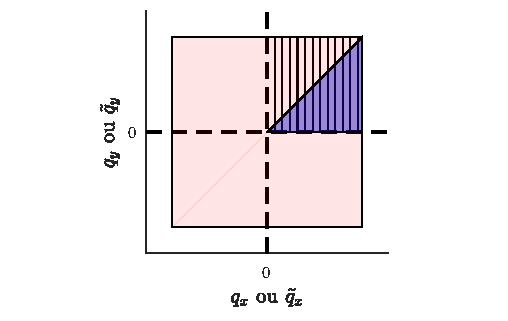
\includegraphics[width=0.95\columnwidth]{SurfUtile.pdf}
\end{center}
\vspace*{-22pt}
\caption{(rouge transparent) Zone complète sur laquelle il faudrait définir les fonctions sans symétrie. (bleue) Zone dans laquelle il suffit de définir numériquement les fonctions. Les symétries permettent donc de "réduire" le problème à un espace plus petit en impulsion.}
\label{fig:SurfUtile}
\end{figure}


\subsection{Interpolation de Tchebytchev}

Afin de pouvoir calculer avec précision les intégrales $J$, $\bJ$, $\tJ$ apparaissant dans les équations nous avons choisi d'interpoler la fonction $\Delta_k$ ainsi que ses dérivées et ses pendants adimensionnées dans le plan des impulsions. Comme annoncé, pour cela nous réutilisons encore une interpolation de Tchébytchev adaptée en dimension 2. 

\subsubsection{Décomposition}

Nous rappelons ici une propriété justifiant l'utilisation des polynômes de Tchebytchev comme polynômes d'interpolation en dimension 2.\\

\noindent
\textbf{Décomposition de Tchebytchev 2D.} 
{\itshape  Soient $a$, $b$ deux réels tels que $b>a$. Soit $f : [a,b]^2 \rightarrow \R$ une fonction continue aux variations bornées (comme définies en \cite{Tchebychev}). On suppose que l'une des dérivées partielles de de $f$ existe et est bornée dans $[a,b]$. Alors il existe une suite des coefficients réels $\{c_{ij}\}_{(i,j) \in \N^2}$ tels que la série $f_n$ définie par :
\begin{equation}
\begin{split}
f_n(x,y) = \sum_{i=0} ^{n} \sum_{j=0} ^{n} c_{ij} T_i\(\frac{2x-a-b}{b-a}\)T_j\(\frac{2y-a-b}{b-a}\)
\end{split}
\end{equation}
converge uniformément vers $f$ quand $n \rightarrow +\infty$.}\\


Ce théorème et sa démonstrations se trouvent dans l'ouvrage \cite{Tchebychev, Masson1980} dans le cas $a=-1$, $b=1$. La généralisation à $a$ et $b$ ($b>a$) quelconques est immédiate. Considérons le schéma semi-discrétisés en temps des équations. Pour des raisons similaires à ce qui a été fait en \refsec{} (\refann{}) nous travaillons alors avec des fonctions de classe $\Cc^1$ selon les variables $\phi$, $p_x$ et $p_y$ (ou leurs équivalents adimensionnés). Il semble alors possible de tirer profit de cette propriété avec nos fonctions \cite{Masson1980} en utilisant une telle décomposition. 

\vspace*{11pt}

\subsubsection{Décomposition méthode 1}

Soient $a$, $b$ deux réels ($b>a$). Soit $f$ une fonction de $[a,b]^2$ dans $\R$. Dans un premier temps nous avons opté pour un algorithme de recherche direct des coefficients $c_{ij}$ de sa décomposition en série de polynômes de Tchebytchev basée sur la méthode 1D. Supposons, en effet, que l'on veuille effectuer une décomposition à l'ordre $n_c -1$ et donc écrire
\begin{equation}
  f(x,y) \simeq \sum_{i=0}^{n_c-1}\sum_{j=0}^{n_c-1} c_{ij} T_i\(\frac{2x-a-b}{b-a} \)T_j\( \frac{2y-a-b}{b-a}\)
  \label{eq:dec}
\end{equation}

Pour trouver la valeur des coefficients de la matrice $((c_{i,j}))_{i,j}$ on prend les ensembles des racines du polynôme de Tchebytchev  de degré $n_c$, $\left\{x_m\right\}_{0\le m \le n_c-1}$ et $\left\{y_n\right\}_{0\le m \le n_c-1}$ et on impose \refeq{dec} en ces points, ce qui revient aussi à écrire,
\begin{equation}
\begin{split}
   f\(\frac{a+b}{2} + x_m\frac{a-b}{2}, \frac{a+b}{2} + y_n\frac{a-b}{2}\) =  \\
    \sum_{i=0}^{n_C-1} \sum_{j=0}^{n_c-1}  c_{ij} T_i\(x_m\) T_j\(y_n\)
\end{split}
\end{equation}
En utilisant les relations des polynômes de Tchebytchev on peut alors determiner les coefficients de la matrice $((c_{ij}))_{i,j}$ avec les formules
\begin{equation}
\begin{split}
 c_{ij} = & \frac{A_{ij}}{n_c^2}  \sum_{m=0}^{n_c-1}  \sum_{n=0}^{n_c-1}  T_i \(x_m\) T_j\( y_n \) \\
 & \times f\(\frac{a+b}{2} + x_m\frac{b-a}{2}, \frac{a+b}{2} + y_n\frac{b-a}{2}\)  
\end{split}
\end{equation}
Avec la notation
\begin{align}
  A_{ij} = 
  \begin{cases}
    1 \quad \text{si } i = j = 0 \\
    2 \quad \text{si } i = 0 \text{ et } j \neq 0 \\
    2 \quad \text{si } i \neq 0 \text{ et } j = 0 \\
    4 \quad \text{si } i \neq 0 \text{ et } j \neq 0 \\
  \end{cases}
\end{align}

Cette méthode est couteuse puisque pour calculer l'ensemble des coefficients de $((c_{ij}))_{i,j}$ cela demande un algorithme de complexité évoluant en $\mathcal{O}(n_c^2)$. En outre pour ensuite obtenir $f(x,y)$ en tout point $(x,y) \in [a,b]^2$, il faut utiliser un algorithme qui est aussi de complexité $\mathcal{O}(n_c^2)$. Ce pourquoi, afin d'obtenir de meilleurs temps de calcul sur les interpolations à précision fixée nous avons implémenté la deuxième méthode suivante.


\vspace*{11pt}

\subsubsection{Décomposition méthode 2}

Il existe une méthode plus astucieuse que celle développée précédemment, inspirée de ce qui est mis en place dans le paquet \textit{chebfun} permettant justement de traiter les interpolations de Tchebytchev sous Matlab. Cette méthode est développée dans \cite{TownsendThesis}. 

Au lieu de faire directement une décomposition sur une base tensorielle de polynômes de Chebychev on commence par réaliser une approximation de rang faible de la fonction que l'on souhaite approximer. Plus précisément, on considère les ensembles des racines de Tchebytchev $\left\{x_m\right\}_{0\le m \le n_c-1}$ et $\left\{y_n\right\}_{0\le m \le n_c-1}$. Alors on peut former la matrice 
\begin{equation}
	\mat{F} = \( \(  f\(\frac{a+b}{2} + x_m\frac{b-a}{2}, \frac{a+b}{2} + y_n\frac{b-a}{2}\)     \)  \)_{m,n}
\end{equation}
et faire de cette matrice une approximation de rang faible par élimination Gaussienne avec l'algorithme suivant, en $\varepsilon$ de l'ordre de la précision machine.

\begin{algorithm}[H]
  \begin{algorithmic}[1]
    \STATE Initialisation : $\mat{E}^0 = \mat{F}$; $\mat{F}_0 = 0$; $k = 1$;
    \WHILE{ ${\| \mat{E}^k \|}_{\infty} < \varepsilon {\| \mat{E}^0 \|}_{\infty}$ }
    \STATE $(i_k, j_k) =  {\text{argmax}}_{(i,j)} \left\{\left| \mat{E}^{k-1}_{i,j} \right| \right\}$
    \STATE $\mat{C}^k_{j} = \mat{E}^k_{i_k,j}$;  $\mat{R}^k_{i} = \mat{E}^k_{i,j_k}$; $d_k = \mat{E}^k_{i_k,j_k}$
    \STATE $\mat{E}^k_{i,j} = \mat{E}^{k-1}_{i,j} - d_k^{-1}\mat{C}^k_{j}\mat{R}^k_{i}$
    \STATE $\mat{F}^k_{i,j} = \mat{F}^{k-1}_{i,j} + d_k^{-1}\mat{C}^k_{j}\mat{R}^k_{i}$
    \ENDWHILE
  \end{algorithmic}
\end{algorithm}

Notons $Q$ ($Q \le n_c$) le rang de l'approximation obtenue. La matrice $\mat{F}$ peut être approximée, à la précision machine, par  
\begin{equation}
\mat{F} \simeq \tilde{\mat{F}} = \sum_{j=1}^Q d_j \mat{C}^j \mat{R}^j
\end{equation}
Comme nous ne connaissons exactement la fonctions $f$ discrétisée qu'aux points d'interpolation cela revient au même que d'écrire que nous avons décomposé $f$ comme une somme de produits de fonctions à une variable,
\begin{equation}
f(x,y) \simeq \sum_{j=1}^Q d_jc^j(y)r^j(x)
\end{equation}
On peut alors décomposer les fonctions $c_j$ et $r_j$ sur une base de polynômes de Chebychev comme on peut le faire pour toute fonction d'une seule variable. La décomposition est dite "une opération de produit tensoriel". \\


Afin de récupérer la valeur de $f$ en un point quelconque $(x,y) \in [a,b]^2 $ nous utilisons simplement la méthode de Clenshaw à une variable sur les fonctions $c^j$ et $r^j$ déjà mentionnée en \refsec{}. Ainsi l'algorithme de décomposition possède une complexité en $\mathcal{O}(Q n_c)$ et il en est de même pour le calcul de $f$ en $(x,y) \in [a,b]^2$. Le gain n'est pas extrêmement important pour ce qui est du temps de calcul mais il a eu son importance pour permettre d'atteindre des résultats convenables en des temps raisonnables. En effet nous avons pour une grande partie de la résolution $Q < n_c$ de par la régularité des fonctions. \\



\subsection{Le calcul des intégrales} 

Pour calculer numériquement les différentes intégrales nous nous servons des propriétés de symétrie que nous avons détaillées des différentes fonctions. Cependant il s'est aussi posé le choix de la méthode utilisée pour réaliser cette quadrature. Comme les intégrales sont à calculer sur une forme géométrique simple, un carré (ou la moitié d'un carré), nous avons opté pour utiliser une version "tensiorielle" d'une quadrature à une dimension de Gauss-Legendre. Cependant nous avions eu d'autres idées que nous n'avons pas retenues pour diverses raisons expliquées ci-dessous.


\subsubsection{Le choix de la quadrature}

On interpole la partie en impulsion des fonctions avec des polynômes de Tchebytchev et on utilise toujours une méthode pseudo-specrtrale\footnote{c'est à dire que l'on connait à chaque pas de temps la valeur de la fonction au points d'interpolation de Tchebythchev, ainsi que les coefficients de son développement en série de polynômes de Tchebytchev}. Il semble donc naturel de se demander si la quadrature de Gauss-Legendre est vraiment la mieux adaptée. En effet, pour gagner du temps et utiliser directement la connaissance de la fonction aux points d'interpolation nous avons penser au calcul d'intégrale par la \emph{première règle de Fejer} \cite{} qui permet cela. En effet les points de quadrature de cette méthode sont ceux de l'interpolation de Tchebytchev avec les polynômes de première espèce, comme nous le faisons ici. Ainsi on d'affranchi du calcul par la méthode de Clenshaw en $\mathcal{O}(n_c^2)$ de la fonction à intégrer. 
 
Cependant cette méthode s'est avérée être inefficace puisque il faut de manière générale plus de points pour obtenir la même précision qu'une quadrature de Gauss Legendre. De plus le passage le plus long du code est le calcul des intégrales $J_3$, $\bJ_3$, $\tJ_3$ et cette quadrature ne permet pas de réaliser ce calcul plus vite. En effet pour calculer cette intégrale il faut évaluer les fonctions $\Delta_k$, $\bDelta_k$, $\tY_k$ en des points $(p_x+q_x, p_y+q_y,\phi)$, ce qui, à cause de la somme des impulsion nécessite, d'interpoler. Et ce, avec n'importe quelle discrétisation en impulsion faite sur une grille de points non régulièrement espacés. \\

Une alternative complètement différente aurait alors consisté à ne pas utiliser une discrétisation en impulsion sur une base de polynôme de Tchebytechv mais plutôt une discrétisation en impulsion sur une grille de points régulièrement espacés. Il est alors possible d'écrire en deux dimensions une quadrature qui ne demande de connaitre la fonction à intégrer qu'aux points de discrétisations et ceci même pour la fonction $J_3$ et ses versions adimensionnées (en effet si  $p_x$ et $q_x$ appartiennent à la grille de discrétisation alors $p_x+q_x$ aussi\footnote{En utilisant la périodicité des fonctions on se ramène encore à un point de la grille quand $p_x+q_x$ en dépasse}). Cependant les quadratures alors testées (basé sur une triangulation régulière de l'espace et des descriptions par éléments finis) demandaient un nombre trop important de points de discrétisation pour obtenir des précisions suffisantes en comparaison de la quadrature de Gauss-Legendre.

% Insert image of calculation by these two quadrature  

\vspace*{11pt}



\subsubsection{Calcul des intégrales $I$, $\bI$, $\tI$}

Soit $a>0$ un réel. Soit $f$ une fonction de $[-a, a]^2$ à valeurs dans $\R$. On suppose que $f$ est symétrique par rapport à l'axe des $x=0$, à l'axe des $y=0$ et à l'axe $x=y$. Nous cherchons alors une quadrature pour integrer $f$ sur son domaine de définition. Pour commencer, en utilisant les deux premières symétries,
\begin{equation}
\int_{-a}^{a} \int_{-a}^{a} f(x,y) \, \dd x \, \dd y = 4 \int_{0}^{a}  \int_{0}^{a} f(x,y) \, \dd x \, \dd y
\end{equation} 
\commentout{
On peut alors faire le changement de variable affine  $\(\tilde{x}, \tilde{y}\) \rightarrow \(2x/a -1, 2y/a -1\) $ donnant,  
\begin{equation}
\begin{split} 
  \int_{0}^{a}  \int_{0}^{a}  f(x,y) \, & \dd x \, \dd y = \\
 \frac{a^2}{4} \int_{-1}^{1} & \int_{-1}^{1} f\(\frac{a}{2}\(\tilde{x}+1\),\frac{\pi}{2}\(\tilde{y}+1\)\) \, \dd \tilde{x}  \, \dd \tilde{y} 
\end{split}
\end{equation}
Les intégrales sur le carré unité $[-1,1] \times [-1, 1]$ sont alors calculées avec une quadrature \textit{tensorielle} obtenue à partir d'une quadrature 1D :
}

Ce qui se calcule en utilisant une quadrature de Gauss-Legendre sur chaque dimension d'intégration, 
\begin{equation}
\begin{split}
 \int_{-a}^{a} \int_{-a}^{a} f(x,y) \,&  \dd x \, \dd y \simeq \\ 
 a^2\sum_{i=0}^{n_{gl}} & \sum_{j=0}^{n_{gl}}w_i w_j f(\frac{a}{2}\(\xi_i+1\), \frac{a}{2}\(\xi_j+1\))
\end{split}
\end{equation}

Où $\{\xi_i\}_{i \in \bbrac {1, n_{gl}}}$ sont les points de la quadrature et  $\{w_i\}_{i \in \bbrac {1, n_{gl}}}$ les poids correspondants. Par construction, $((w_i w_j))_{i,j}$ est une matrice symétrique et par symétrie de $f$ par rapport à la première bissectrice nous pouvons alors réduire la double somme par, 
\begin{equation}
\begin{split}
 \int_{-a}^{a} \int_{-a}^{a} f(x,y) \,&  \dd x \, \dd y \simeq \\ 
 a^2\sum_{i=0}^{n_{gl}} & \sum_{j=0}^{i-1}w_i w_j 2 f(\frac{a}{2}\(\xi_i+1\), \frac{a}{2}\(\xi_j+1\)) \, + \\
a^2\sum_{i=0}^{n_{gl}} & w_i^2f(\frac{a}{2}\(\xi_i+1\), \frac{a}{2}\(\xi_i+1\))
\end{split}
\end{equation}
Ce qui permet de réduire le temps de calcul en réduisant légèrement le nombre d'opérations à effectuer.

\vspace*{11pt}




\subsubsection{Calcul des intégrales $J$,$\bJ$,$\tJ$ }

Soit $a>0$. Soit $(b,c) \in [0,a]^2$. Soit maintenant $g$ et $h$ deux fonctions de $\R^2$ dans $\R$ et  $g$ définie sur $[-a, a]^2$  par $g : (x,y) \rightarrow u(x+b, y+c)$. On suppose, comme précédemment, que $g$ et $h$ sont symétriques par rapport à l'axe $x=0$, à l'axe $y=0$ et à l'axe $x=y$. On fait aussi l'hypothèse qu'elles sont $2\pi$ periodiques. Nous cherchons alors une formule pour intégrer $g\times h$ sur $[-a, a]^2$. Pour cela remarquons que
\begin{equation}
\begin{split}
 & \int_{-a}^{a} \int_{-a}^{a} g(x,y) h(x,y) \,  \dd x \, \dd y  = \\
 \int_{0}^{a} & \int_{0}^{a} [u(x+b, y+c) + u(x+b, y-c)] h(x,y) \, \dd x \, \dd y \, + \\ 
\int_{0}^{a} & \int_{0}^{a} [u(x-b, y+c) + u(x-b, y-c)] h(x,y)  \, \dd x \, \dd y 
\end{split}
\end{equation}

Et on adopte encore la même quadrature que pour les intégrales $I$, $\bI$, $\tI$. Cependant remarquons que ce calcul impose de connaitre les valeurs de $u$ en des points $(x \pm b, y\pm c)$ qui sont en dehors du carré $[0, a]^2$. Or, à cause de la discrétisation, $u$ est une fonction que l'on connait par sa décomposition en série de tchebytchev sur $[0,a]^2$, ainsi, on ne peut pas connaitre la valeur de $u$ en tout $(x\pm b, y\pm c)$. Lorsque l'on s'intéresse au calcul de $J$ cela ne pose pas de problèmes car on peut utiliser la périodicité des fonctions (raison pour laquelle nous résolvons en premier lieu le système $\Ec_1$ dimensionné). En revanche pour $\bJ$ et $\tJ$ , la périodicité est brisée dans les équations et nous sommes obligé d'extrapoler $u$ en dehors de $[0,a]^2$





\subsection{Dérivées numériques en champ }

Les dérivées numériques e champ $\phi$ ou $\tphi$ sont encore calculées sur 5 points pour essayer d'avoir la meilleure  précision possible. Cependant comme nous l'avons mentionné nous avons du dans des premières versions du code utilisé des dérivées sur trois points à cause d'instabilité en bords des grilles de discrétisation. Nous pouvons justifier rapidement la présence de telles instabilités. En effet, comme nous ne disposons pas de conditions aux bords pour nos équations il se trouve que nous sommes obligés d'utiliser des schémas de discrétisation à cinq points fortement décentrés sur les bords, n'utilisant que des points à l'intérieur de la grille.\\


Or, pour étudier simplement ces schéma nous les appliquons à une équation d'advection du type $\partial_x u + a \partial_t u = 0$ et nous en faisons une analyse de Von-Neumann. Il est donc possible de calculer les facteurs d'amplification de ces schémas, comme en \refig{FacAmp}, montrant que les schémas à 5 points peuvent rapidement introduire des instabilités.\\

Bien que nos équations soient assez éloignées d'une simple équation d'advection cette rapide étude permet de donner une idée de la raison pour laquelle l'utilisation de dérivées à trois points a probablement permis de résoudre des problèmes d'instabilité en bord de grille en champ.

\begin{figure}[H]
\begin{center}
	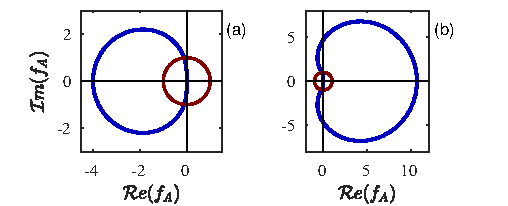
\includegraphics[width=0.95\columnwidth]{FacAmp.pdf}
\end{center}
\caption{(a) Facteur d'amplification $f_A$ du schéma décentré gauche à 3 points pour la dérivée première obtenu par analyse de Von-Neuman pour $a=1$ (bleu). Le cercle rouge représente le cercle unité. (b) Même chose pour le schéma décentré gauche à 5 points. Les courbes bleues restent dans le cercle rouge pour des modes de fréquence $|\theta| < \pi/4$ dans les deux cas, mais en dehors du cercle unité $f_A$ conserve une amplitude bien plus modérée dans le cas (a). Ainsi nous pouvons penser que dans notre schéma le schéma à 3 points à plus de chance d'être stable pour un même pas de discrétisation.}
\label{fig:FacAmp}
\end{figure}


\section{Resultats : Ising 2D}

\subsection{Complexité algorithmique et parallélisation - problème de rapidité} 

Comme pour le modèle continu $O(N)$ il est possible de paralléliser le code en utilisant de l'openMP \cite{} grain fin sur les boucles en champ. En revanche, à cause de la quadrature précise que l'on souhaite avoir sur le calcul des intégrales $J$, sans parallélisation, le temps de calcul se trouve évoluer en $\mathcal{O}( Q_\text{max} \times n_c^3 \times n_{gl}^2 \times n_{\phi})$. Où $n_{\phi}$ est le nombre de point de discrétisation en $\phi$ et $\tphi$, et $Q_{max}$ est le rang maximal nécessaire dans tout le code lors de l'approximation de rang faible de \refsec{GE}. Pour le vérifier nous avons tracé la courbe \refig{timeNc}


Ainsi nous pouvons bien constater l'évolution  problématique du temps de calcul de cet algorithme de résolution. En revanche nous avons aussi étudié l'effet de la parallélisation sur les points de discrétisation en champ $\phi$. Comme attendu nous obtenons une décroissance en $\sim 1/n_{proc}$ ou $n_{proc}$ est le nombre de processeur utilisé. Le résultat est visible en \refig{timeScal}.

Enfin, le nombre de processeurs sur lesquels peuvent être parallélisé le programme est bridé par le nombre de point de la discrétisation en champ. Ainsi pour tenter d'augmenter la vitesse d'exécution nous avons réalisé une version du code avec une parallélisation MPI \cite{} de la boucle en champ et une parallélisation OpenMP des boucles de la quadrature de l'intégrale $J$, $\bJ$ ou $\tJ$. Il s'avère qu'alors il faut communiquer un nombre de données trop important entre les processeurs, le code s'en trouvait alors ralenti, voire inutilisable. 

\begin{figure}[H]
\begin{center}
	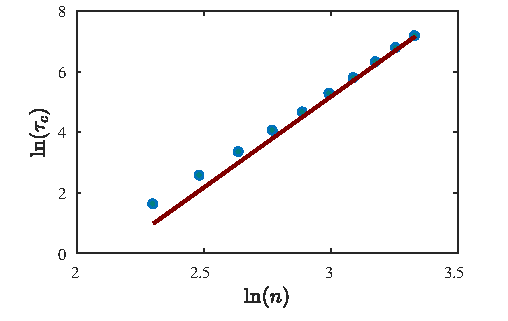
\includegraphics[width=0.95\columnwidth]{ComplexiteTemps.pdf}
\end{center}
\caption{(Points bleus) Logarithme du temps de calcul mesuré $\tau_c$ de 10 pas de temps du code en fonction du nombre de points d'intégration et d'interpolation, avec $n_\phi$ fixé. On a pris $n_c = n_{gl} = n$. (Ligne rouge) droite d'équation $y=6x+b$ avec $b$ une constante. Il semble que les points se rapproche du comportement de la droite et ainsi que l'on ait $t_c \propto n^6$. Un interpolation linéaire sur les données dont on dispose donne plus précisément $t_c \propto n^{5,7} $   }
\label{fig:timeNc}
\end{figure}


\begin{figure}[H]
\begin{center}
	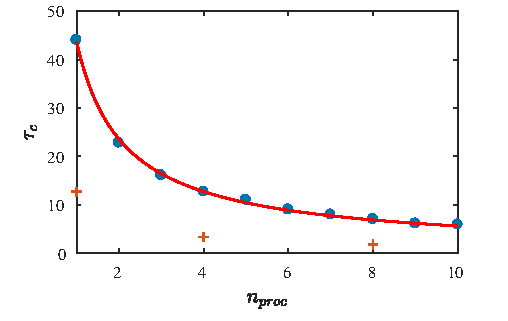
\includegraphics[width=0.95\columnwidth]{Scalabilite.pdf}
\end{center}
\caption{Évolution du temps de calcul $\tau_c$ avec le nombre $n_{proc}$ de processeurs utilisés. (points verts) En exécutant le code sur les ordinateurs du laboratoires limitées, pour celles que nous avons pu utiliser, à 10 ou 12 cœurs. () En exécutant le code sur le calculateur Mesu. Les courbes continues représentent les régressions linéaires. Nous obtenons $\tau_c \sim n_{proc}^{0.88}$ et $\tau_c \sim n_{proc}^{0.98}$ sur Mesu. }
\label{fig:timeScal}
\end{figure}



\subsection{Problème de précision des intégrales}


A cause de la complexité des algorithmes il n'est pas possible de choisi $n_c$ et $n_{gl}$ aussi grand qu'on le souhaite pour obtenir la precision voulue. Au début nous pensions qu'un nombre faible de points suffiraient mais il s'avère que ce n'est pas spécialement le cas. En effet nous avons dû utiliser le calculateur Mesu \cite{} de l'université Pierre et Marie Curie pour pouvoir paralléliser notre programme sur 48 ou 96 coeurs et pouvoir augmenter $n_c$ et $n_{gl}$ jusqu'à 22 sans dépasser les 72 heures permises pour une simulation sur la machine. Nous avons comparer les résultats obtenus pour différentes simulations en fixant $n_c = n_{gl} = n$ (Il s'avère que prendre $n_c \neq n_{gl}$ ne change pas en mieux les résultats). L'influence de $n$ se trouve en \refig{etaErr}.

\begin{figure}[H]
\begin{center}
	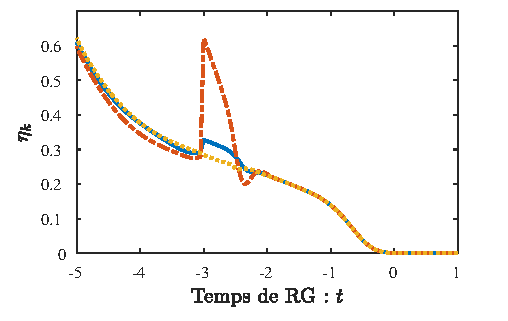
\includegraphics[width=0.95\columnwidth]{EtakErrMesu.pdf}
\end{center}
\caption{Évolution de $\eta_k$ en fonction de $t$ pour différentes valeurs du nombre de point d'interpolation et d'intégration. (rouge discontinu) $n=14$, (bleu continu) $n=20$, (jaune pointillé) $n=22$. Le trait vertical noir se trouve à $t_b = \ln(k_b/\Lambda)$ correspondant au passage du problème ($\Pc_2$) au ($\Pc_3$). Avec une précision suffisante les courbes devraient être continues cependant ce n'est clairement pas le cas pour $n<22$. Même pour $n=22$ il y a une légère différence, mais surtout un épaulement proche de $t=-6$ que l'on ne saurait expliquer.}
\label{fig:etaErr}
\end{figure}

Ainsi pour $n=22$ les résultats semblent être correct avec toutefois quelques irrégularités. Ceci nous confirme qu'une partie des imprécisions sur les résultats que peut permettre de sortir ce code de simulation sont dues au calcul des intégrales. Malheureusement il n'est pas vraiment possible de quantifier cette erreur et de la comparer aux erreurs qui peuvent provenir aussi d'une discrétisation en champ pas assez précise ou d'un pas de temps trop élevé. \\



\subsection{Estimation de la température critique et de l'exposant critique $\eta$}

Enfin, malgré les erreurs que nous avons pu observer, provenant d'une précision non suffisante dans les calculs des intégrales nous avons tenté de récupérer la valeur de la température critique et de l'exposant $\eta_k$ du modèle tout de même. Ainsi en utilisant $n_c = n_{gl} = 22$ nous avons obtenu une température critique 

\begin{equation}
T_c^{BMW}  = (2.3525 \pm 0.025)J/k_B
\end{equation}

Nous savons que la température critique théorique attendu est de $T_c^{th} = 2.2691 J/k_B$. Nous avons donc un résultat proche du résultat attendu avec une erreur 

\begin{equation}
	err = \frac{ |T_c^{BMW} - T_c^{th}|}{T_c^{th}} = 3.5 \%
\end{equation}


Comme nous pouvons le voir en \refig{etaMesu}, en plus de nous donner la température critique, le code nous permet aussi de retrouver $\eta$ autour de $0.25$ pour $d=2, N=1$ comme nous l'avions déjà déterminé en \refsec{}

\begin{figure}[H]
\begin{center}
	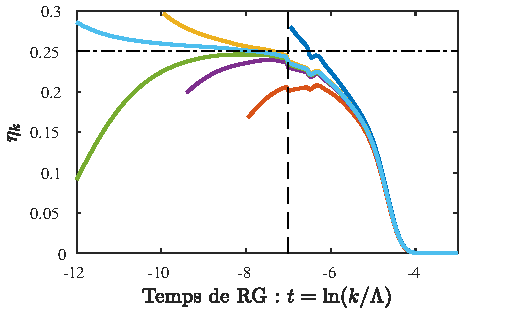
\includegraphics[width=0.95\columnwidth]{MesuRes.pdf}
\end{center}
\caption{Évolution de $\eta_k$ en fonction de $t$ pour différentes valeurs de la températue $T$ du système (la courbe se lit de droite à gauche). $n_c=22$, $n_{gl} = 22$.  Le trait vertical noir se trouve à $t_b = \ln(k_b/\Lambda)$ correspondant au passage du problème ($\Pc_2$) au ($\Pc_3$). Le trait horizontal noir correspond à la valeur théorique $\eta = 0.25$ attendue. }
\label{fig:etaMesu}
\end{figure}


\section{Conclusion}

Nous avons réussi a reprendre un code de simulation d ...

\vfill

\pagebreak

\bibliographystyle{plain}
\bibliography{Rapport}


\end{multicols}


\pagebreak

\appendix


\begin{multicols}{2}
\section{Outils pour le développement des équations}

\label{ann:outils}

\subsection{Transformée de Fourier}

On rappelle ici les notations utilisée pour définir les transformées de Fourier. Pour cela on considère $\varphiv$ une application de $L^2(\R^d)^N$. On définit alors la transformée de Fourier de $\varphiv$, notée $\hat{\varphiv}$ ou $\text{TF}[\varphiv]$ par, 

\begin{equation}
  \forall \qv \in \R^d \quad \hat{\varphiv}(\qv) = \text{TF}[\varphiv](\qv) = \int_{\R^d} \varphiv(\rv) e^{-i\qv.\rv}\dd \,\rv
\end{equation}
Avec la relation inverse,
\begin{equation}
  \forall \rv \in \R^d \quad \varphiv(\rv)  = \text{TF}^{-1}[\hat{\varphiv}](\rv) = \frac{1}{(2\pi)^d}\int_{\R^d} \hat{\varphiv}(\qv) e^{i\qv.\rv}\dd \,\qv
\end{equation}
On utilise alors la notation plus compacte 
\begin{equation}
  \frac{1}{(2\pi)^d}\int_{\R^d} ... \dd \,\qv \equiv \int_\qv ... \quad \text{et} \quad  \int_{\R^d} ... \dd \,\rv \equiv \int_\rv ... 
\end{equation}

Dans le cas ou l'on a des fonctions définies non pas sur $\R^d$ mais sur un domaine $\Omega \subset \R^d$ fini alors nous aurons les mêmes propriétés avec la relation "d'équivalence"  
\begin{equation}
	 \int_{\qv} ... \overset{\text{$\Omega$ fini}}{\quad \longrightarrow \quad } \frac{1}{\Omega} \sum_{\qv} ...
\end{equation}
Remarquons que lorsque l'on introduit la transformée de Fourier (\refsec{}) pour l'utiliser dans le RG les fonctions $\varphiv$ sont tout d'abord définies sur un ouvert $\Omega$ fini mais par des considérations physique, en passant à "la limite thermodynamique" on en vient à considèrer $\Omega$ comme devenant $\R$ tout entier. En outre, dans le cas où $\varphiv \in \Sr'(\R^d)^N$ (espace des distributions tempérées) on étend la notion de transformée de Fourier $\hat{\varphiv}$ de $\varphiv$ à l'aide du crochet de dualité, 
\begin{equation}
  \forall u \in \Sr(\R^d, \R^N) \quad \left< \hat{\varphiv}, u \right>_{\Sr', \Sr} = \left< \varphiv, \hat{u} \right>_{\Sr', \Sr}
\end{equation}

\vspace*{11pt}



\subsection{Transformée de Fourier Semi-Discrète (TFSD)}

\label{ann:TFSD}

Dans le modèle d'Ising à deux dimensions nous introduisons une transformée de Fourier semi discrète car nous travaillons non pas avec des fonctions mais avec des suites. Ainsi soit $\varphi_\rv \in \ell^2$. On peut définir $\hat{\varphi} \in L^2(\R)$ par  
\begin{equation}
  \hat{\varphi}(\qv) = \sum_\rv \varphi_\rv e^{-i\qv\rv}
\end{equation}
  Avec la relation inverse,
\begin{equation}
 \varphi_\rv = \int_{\R^d} \hat{\varphi}(\qv)  e^{i\qv\rv} \dd\, \qv \equiv \int_\qv \hat{\varphi}(\qv)  e^{i\qv\rv}
\end{equation}
On peut de plus démontrer que cette transformation est une isométrie \cite{}.



\vspace*{11pt}
\subsection{Derivation fonctionnelle}

\subsubsection{Définition}
Soit $U$ et $V$ deux espaces de Banach. Soit $F$ une fonctionnelle de $U$ dans $V$. 
Soit $f \in U$. On appelle, si elle existe, dérivée (au sens de Fréchet) de la fonctionelle $F$ prise en $f$, l'application linéaire continu de $\mathcal{L}(U,V)$, notée $D_fF$ telle que, pour $\eps>0$, 
\begin{equation}
\forall h \in U \quad \lim_{ \eps \rightarrow 0 } \frac{\| F[f+\eps h] - F[f] - \eps D_fF.h\|_V}{\eps}  = 0
\end{equation} 
Dans le cas où $U = L^2(\R^d)^N$ et $V = \R$ alors $D_fF \in U'$ (espace des forme linéaires continues de $U$) et on sait qu'il existe, par le théorème de Frechet-Riesz, une quantité unique que l'on note $\delta F[f]/\delta f \in U'(\simeq U)$ telle que 
\begin{equation}
\forall h \in U \quad D_f F.h = {\left< \derd{F[f]}{f}, h \right>}_{U} = \int \derd{F[f]}{f(\rv)} h(\rv) \dd \, \rv	
\end{equation}

\vspace*{11pt}

\subsubsection{Transformée de Fourier d'une dérivée fonctionnelle}

Soit $F$ une fonctionelle de $U = L^2(\R^d)^N$ dans $(\R,|.|)$ et $\varphiv \in U$.
Soit $\rv \in \R^d$.
Alors, 
\begin{equation}
  \derd{F}{\varphiv(\rv)} = \int_{\qv} \derd{F}{\hat{\varphiv}(-\qv)} e^{i\qv.\rv} = \text{TF}^{-1} \left[ \derd{F}{\hat{\varphiv}(-\qv)} \right](\rv) 
\end{equation} 
Et réciproquement nous avons alors aussi, pour $\pv \in \R^d$,  
\begin{equation}
  \derd{F}{\hat{\varphiv}(-\pv)} = \int_{\rv} \derd{F}{\varphiv(\rv)} e^{-i\pv.\rv} = \text{TF} \left[ \derd{F}{\varphiv(\rv)} \right](\pv) 
\end{equation} 

\vspace*{11pt}
%\noindent
{\footnotesize 
\noindent
En effet, par la règle de la chaine de la dérivation de Fréchet nous pouvons écrire, 
\begin{equation}
  \forall \hv \in U \quad D_{\varphiv} F. \hv = D_{\hat{\varphiv}} F. D_{\varphiv} \hat{\varphiv}.\hv 
\end{equation}
Cependant, $\hat{\varphiv}$ est une fonctionnelle de $\varphiv$ (par définition de la TF) de $U$ dans $U$ qui est linéaire en $\varphiv$. Soit $\eps >0$, 
\begin{equation}
  \forall \hv \in U \quad \hat{\varphiv}[\varphiv + \eps \hv] - \hat{\varphiv}[\varphiv] = \eps \hat{\hv} 
\end{equation} 
Il vient directement, par définition de la dérivation au sens de Frechet, $D_{\varphiv} \hat{\varphiv} .\hv = \hat{\hv}$.  
Ainsi,  $D_{\varphiv} F .\hv = D_{\hat{\varphiv}}F.\hat{\hv}$.  On peut alors écrire, 
\begin{align}
  \forall \hv \in U  \quad D_{\varphiv} F .\hv & = \int_{\qv} \derd{F}{\varphiv(\qv)} \int_{\rv} \hv(\rv) e^{-i\qv.\rv} \\
  \forall \hv \in U  \quad D_{\varphiv} F .\hv & = \int_{\rv} \int_{\qv} \derd{F}{\varphiv(\qv)} e^{-i\qv.\rv } \hv(\rv)
\end{align}
}



\subsection{Opérateurs à noyaux}

Nous détaillons dans cette sections quelques propriétés élémentaires des opérateurs à noyaux. Pour plus de détails on pourra regarder \cite{}. Ceci permet de comprendre quelques unes des étapes dans la détermination des équations de flot et BMW. \\



\subsubsection{Définition}

On appelle $S$ un operateur a noyaux, une application de $(L^2(\R^d))^N$, telle que pour tout $(i,j) \in \bbrac{1,N}^2$, il existe une application $A_{i,j} \in L^2(\R^d\times\R^d)$ telle que,  pour tout $\varphiv \in (L^2(\R^d)^N$ et $\rv \in \R^d$
 \begin{equation}
  S[\varphiv]_i(\rv) = \int_{\rv'} \sum_{j=1}^{N} A_{i,j}(\rv,\rv')\varphi_j(\rv')
 \end{equation}
 La matrice $A : (\rv,\rv') \rightarrow ((A_{i,j}(\rv,\rv')))_{i,j}$ est appelée noyau de $S$.  On identifiera alors dans les notations $S$ et $A$ indépendamment. Par Cauchy-Schwartz cette définition a bien  un sens. De plus, on peut montrer que $S$ et est un endomorphisme de $(L^2(\R^d)^N$. Pour plus de clarté, nous utiliserons par la suite la notation d'Einstein : on n'écrit plus la somme sur $j$ dans l'expression de $S$, et de manière générale lorsque un indice est répété dans une expression on suppose qu'il est sommé de $1$ à $N$, 
  \begin{equation}
  S[\varphiv]_i(\rv) \equiv \int_{\rv'} A_{i,j}(\rv,\rv')\varphi_j(\rv')
 \end{equation}
 



\vspace*{11pt}

\subsubsection{TF d'un opérateur à noyau}

Nous avons vu que $S$ définie comme précédemment était un endomorphisme de $(L^2(\R^d)^N$. Ainsi il est possible d'en définir la transformée de Fourier. Introduisons tout d'abord la transformée de Fourier du noyaux, pour $(i,j) \in \bbrac{1,N}^2$ et $(\qv, \qv') \in (\R^d)^2 $
\begin{equation}
	 \hat{A}_{i,j}(\qv, -\qv') = \iint_{\rv,\rv'} A_{i,j}(\rv,\rv')\,e^{-i\qv.\rv} \, e^{-i \qv'.\rv'} 
\end{equation}
Ce qui implique alors 
\begin{equation}
	 \hat{S}[\varphiv]_i(\qv) = \int_{\qv'} \hat{A}_{i,j}(\qv, -\qv') \hat{\varphi}_j(\qv')
\end{equation}



{\footnotesize
\noindent
En effet, ceci ce démontre en développant le calcul de la transformée de Fourier. Soit $\qv \in \R^d$, $i \in \bbrac{1,N}$
\begin{align}
 \hat{S}[\varphiv]_i(\qv)  = & \int_{\rv} \int_{\rv'} A_{i,j}(\rv,\rv')\varphi_j(\rv') e^{-i\qv\rv}  \\
\hat{S}[\varphiv]_i(\qv)  = & \iint_{\rv, \rv'} \int_{\qv'} A_{i,j}(\rv,\rv') \hat{\varphi}_j(\qv') e^{i\qv'\rv'} e^{- i\qv\rv} \\
 \hat{S}[\varphiv]_i(\qv)  = &   \int_{\qv'} \hat{\varphi}_j(\qv') \left\{ \iint_{\rv, \rv'} A_{i,j}(\rv,\rv')  e^{i\qv'\rv'} e^{- i\qv\rv}  \right\}  \\
\hat{S}[\varphiv]_i(\qv) = & \int_{\qv}  \hat{\varphi}_j(\qv') \hat{A}_{i,j}(\qv, -\qv')
\end{align}
}

\vspace*{11pt}

\subsubsection{Composition de deux opérateurs}

Considérons deux opérateurs à noyaux, $S$ et $T$ de noyaux respectifs $A$ et $B$. La composition de ces deux opérateurs est définie, pour $\rv \in \R^d$, par
\begin{equation}
 	S . T [\varphiv]_i (\rv) = \int_{\rv'}  \left\{ \int_{\rv''} A_{i,k}(\rv, \rv'')B_{k,j}(\rv'', \rv') \right\} \varphi_j(\rv')
\end{equation}
On notera alors aussi pour $(\rv, \rv') \in (\R^d)^2 $
\begin{equation}
   (A . B)_{i,j} (\rv, \rv') = \int_{\rv''} A_{i,k}(\rv, \rv'')B_{k,j}(\rv,'' \rv') 
\end{equation}
Par transformée de Fourier, et par un calcul analogue à celui fait pour un simple noyau, il vient, pour $(\qv, \qv') \in (\R^d)^2$,
\begin{equation}
	\widehat{(A . B)}_{i,j}(\qv, \qv') =\int_{\qv''} \hat{A}_{i,k}(\qv, \qv'')\hat{B}_{k,j}(-\qv'', \qv') 
\end{equation}



\vspace*{11pt}

\subsubsection{Trace d'un opérateur à noyau}

On définit la trace d'un opérateur $S$ de noyaux $A$ par
\begin{equation}
  \text{Tr}\, S \equiv \text{Tr} \, A = \int_{\rv} A_{i,i}(\rv,\rv) 
\end{equation}
Nous pouvons alors de manière similaire à ce qui a été fait pour démontrer l'expression de la transformée de Fourier d'un opérateur à noyau, calculer la relation sur la trace de la transformée de Fourier
\begin{equation}
  \text{Tr} \hat{A} =  \int_{\qv} \hat{A}_{i,i}(\qv,-\qv) 
 \end{equation}



\vspace*{11pt}



\subsubsection{Inverse d'un opérateur à noyau}

Soit S un opérateur à noyau de noyaux A. On fait l'hypothèse, sans justifications, que pour les systèmes physiques que l'on étudie il existe une grandeur appelée l'inverse de S, également un opérateur à noyau, endomorphisme de $(L^2(R^d))^N$, notée $S^{-1}$ telle que, pour $i \in \bbrac{1,N}$ et $\varphiv \in (L^2(R^d))^N$, 
\begin{equation}
	\forall \rv \in \R^d \quad S.S^{-1}[\varphiv]_i(\rv) = \varphi_i (\rv)	
\end{equation}

Si $A$ est le noyau de $S$, on note $A^{-1}$ le noyau de $S^{-1}$.

\end{multicols}



\pagebreak



\section{Propriétés des fonctions à discrétiser}



\subsection{Symétries et périodicité des fonctions inconnues}

Partons de l'équation BMW \refeq{flotBMW}. 
\begin{equation}
	\partial_t \Gamma_{k}^{(2)}(\pv, \phi) =  J_3(\pv, \phi) {\( \partial_\phi \Gamma_{k}^{(2)}(\pv, \phi) \)}^2 
	- \frac{1}{2}  I_2(\phi) \, \partial_\phi^{2} \Gamma_{k}^{(2)}(\pv, \phi)
\end{equation}
Soit $u$ une application linéaire, difféomorphisme de classe $\Cc^1$ de $\R^d$ dans $\R^d$ tel que $\text{det(Jac(}u)) = \pm 1$. Supposons que $\Rc_k(u(\qv)) = \Rc_k(\qv)$ pour tout $\qv \in \R^d$ et $k \in ]0, \Lambda]$. On pose le schéma semi-discrétisé d'Euler en temps de l'équation précédente. Il vient, pour $n \in \N$,
\begin{equation}
	 \Gamma_{k_{n+1}}^{(2)}(\pv, \phi) = \Gamma_{k_n}^{(2)}(\pv, \phi) + \delta t \left\{ J_3(\pv, \phi) {\( \partial_\phi \Gamma_{k_n}^{(2)}(\pv, \phi) \)}^2 
	- \frac{1}{2}  I_2(\phi) \, \partial_\phi^{2} \Gamma_{k_n}^{(2)}(\pv, \phi) \right\}
\end{equation}
Soit $\phi \in \R$ fixé. Supposons que pour tout $\pv \in \R^d$ nous ayons $ \Gamma_{k_{0}}^{(2)}(u(\pv), \phi) = \Gamma_{\Lambda}^{(2)}(u(\pv), \phi) = \Gamma_{\Lambda}^{(2)}(\pv, \phi)$.\\
\noindent
 Montrons par induction qu'alors pour tout $\pv \in \R^d$, $ \Gamma_{k_{n}}^{(2)}(u(\pv), \phi) = 
\Gamma_{k_{n}}^{(2)}(\pv, \phi)$ pour tout $n \in \N$.\\

Soit $n \in \N$,  $\pv \in \R^d$ supposons la propriété au vraie au rang $n$, il vient directement 
\begin{equation}
\partial_\phi \Gamma_{k_n}^{(2)}(u(\pv), \phi) = \partial_\phi \Gamma_{k_n}^{(2)}(\pv, \phi) \quad \text{et} \quad \partial_\phi^2 \Gamma_{k_n}^{(2)}(u(\pv), \phi) = \partial_\phi^2 \Gamma_{k_n}^{(2)}(\pv, \phi) 
\end{equation}
De plus nous avons 
\begin{equation}
\begin{split}
	& J_3(u(\pv), \phi) = \int_\qv \partial_t \Rc_{k_n}(\qv) \frac{1}{\Gamma_{k_n}^{(2)}(u(\pv)+\qv, \phi) + \Rc_{k_n}(u(\pv)+\qv)} \(\frac{1}{\Gamma_{k_n}^{(2)}(\qv, \phi) + \Rc_{k_n}(\qv)}\)^2 \\
	& J_3(u(\pv), \phi) = \int_\qv \partial_t \Rc_{k_n}(\qv) \frac{1}{\Gamma_{k_n}^{(2)}(u(\pv)+u\circ u^{-1}(\qv), \phi) + \Rc_{k_n}(u(\pv)+u\circ u^{-1}(\qv))} \(\frac{1}{\Gamma_{k_n}^{(2)}(\qv, \phi) + \Rc_{k_n}(\qv)}\)^2  \\
	& J_3(u(\pv), \phi) = \int_\qv \partial_t \Rc_{k_n}(\qv) \frac{1}{\Gamma_{k_n}^{(2)}(u(\pv + u^{-1}(\qv)), \phi) + \Rc_{k_n}(u(\pv + u^{-1}(\qv)))} \(\frac{1}{\Gamma_{k_n}^{(2)}(\qv, \phi) + \Rc_{k_n}(\qv)}\)^2  \\
	& J_3(u(\pv), \phi) = \int_\qv \partial_t \Rc_{k_n}(\qv) \frac{1}{\Gamma_{k_n}^{(2)}(\pv + u^{-1}(\qv), \phi) + \Rc_{k_n}(\pv + u^{-1}(\qv))} \(\frac{1}{\Gamma_{k_n}^{(2)}(\qv, \phi) + \Rc_{k_n}(\qv)}\)^2 
	\end{split}
\end{equation}
On pose le changement de variable $\qv' = u^{-1}(\qv)$. Nous avons alors $\qv = u(\qv')$ et les relations 
\begin{equation}
	\Rc_{k_n}( u(\qv') ) =  \Rc_{k_n}(\qv'), \quad
	\partial_t \Rc_{k_n}( u(\qv') ) = \partial_t \Rc_{k_n}(\qv') \quad \text{et} \quad
	\Gamma_{k_n}^{(2)}(u(\qv'), \phi) = \Gamma_{k_n}^{(2)}(\qv', \phi)
\end{equation}
De plus si l'intégrale sur $\qv$ est effectué sur un domaine fini $\Dc$ alors on suppose aussi que $u(\Dc) = \Dc$ (i.e. que $u|_{\Dc}$ est aussi un $\Cc^1$ difféomorphisme). Il vient, par unitarité du jacobien de $u$, l'expression de l'intégrale
\begin{equation}
\begin{split}
	& J_3(u(\pv), \phi) = \int_{\qv'} \partial_t \Rc_{k_n}(\qv') \frac{1}{\Gamma_{k_n}^{(2)}(\pv+\qv', \phi) + \Rc_{k_n}(\pv+\qv')} \(\frac{1}{\Gamma_{k_n}^{(2)}(\qv', \phi) + \Rc_{k_n}(\qv')}\)^2 \\
	& J_3(u(\pv), \phi) = J_3(\pv, \phi)
	\end{split}
\end{equation}
Or nous avons
\begin{equation}
\begin{split}
	 & \Gamma_{k_{n+1}}^{(2)}(u(\pv), \phi) = \Gamma_{k_n}^{(2)}(u(\pv), \phi) + \delta t \left\{ J_3(u(\pv), \phi) {\( \partial_\phi \Gamma_{k_n}^{(2)}(u(\pv), \phi) \)}^2 
	- \frac{1}{2}  I_2(\phi) \, \partial_\phi^{2} \Gamma_{k_n}^{(2)}(u(\pv), \phi) \right\} \\
	& \Gamma_{k_{n+1}}^{(2)}(u(\pv), \phi) = \Gamma_{k_n}^{(2)}(\pv, \phi) + \delta t \left\{ J_3(\pv, \phi) {\( \partial_\phi \Gamma_{k_n}^{(2)}(\pv, \phi) \)}^2 
	- \frac{1}{2}  I_2(\phi) \, \partial_\phi^{2} \Gamma_{k_n}^{(2)}(\pv, \phi) \right\} \\
	& \Gamma_{k_{n+1}}^{(2)}(u(\pv), \phi) = \Gamma_{k_{n+1}}^{(2)}(\pv, \phi)
	\end{split}
\end{equation}
Ainsi nous avons montré la propriété. \\

Remarquons que l'hypothèse $\Rc_k(u(\pv)) = \Rc_k(\pv)$ est équivalente à l'hypothèse $\varepsilon(u(\pv)) = \varepsilon(\pv)$ pour tout $\pv \in \R^d$ de par l'expression du régulateur. Ainsi dans la première étude, pour le modèle $\varphi^4$, $\varepsilon(\pv) = \pv^2$, et nous pouvons appliquer la propriété précédente pour tout $u$ ayant la forme d'une rotation dans $\R^d$ : nous avons une symétrie centrale. Dans la deuxième partie, comme $\varepsilon(\pv) = \eo(\pv)$ nous pouvons appliquer la propriété précédente, avec $\varepsilon(u(\pv)) = \varepsilon(\pv)$ pour les fonction $u$ suivantes, 
\begin{equation}
\begin{split}
	u & : (p_x, p_y) \in \R^2 \to (-p_x, p_y) \in \R^2 \\
	u & : (p_x, p_y) \in \R^2 \to (p_x, -p_y) \in \R^2 \\
	u & : (p_x, p_y) \in \R^2 \to (p_y, p_x) \in \R^2  
	\end{split}
\end{equation}
De plus le même raisonnement fonctionne aussi pour montrer la $2\pi$-périodicité des fonctions en impulsion dans le cas Ising 2D et montrer qu'elles peuvent bien être définies sur $\R^2$ tout entier.

\vspace*{11pt}
Soit maintenant $\pv \in \R^d$. Supposons que pour pour tout $\phi \in \R$, nous ayons $ \Gamma_{k_{0}}^{(2)}(\pv, -\phi) = \Gamma_{\Lambda}^{(2)}(u(\pv), -\phi) = \Gamma_{\Lambda}^{(2)}(\pv, \phi)$ (i.e. que ce soit une fonction paire). 
Montrons que pour tout $\phi \in \R$, $\Gamma_{k_{n}}^{(2)}(u(\pv), -\phi) = \Gamma_{k_{n}}^{(2)}(\pv, \phi)$. \\

Soit $n \in \N$, $\phi \in \R$, supposons la propriété vraie au rang $n$, il vient
\begin{equation}
	\partial_\phi \Gamma_{k_{n}}^{(2)}(\pv, -\phi) = - \partial_\phi \Gamma_{k_{n}}^{(2)}(\pv, \phi) \quad \text{et} \quad \partial_\phi^2 \Gamma_{k_{n}}^{(2)}(\pv, -\phi) =  \partial_\phi^2 \Gamma_{k_{n}}^{(2)}(\pv, \phi) 
\end{equation}
De plus nous avons
\begin{equation}
	I_2(-\phi) = \int_\qv \partial_t \Rc_{k_n}(\qv) \(\frac{1}{\Gamma_{k_n}^{(2)}(\qv, - \phi) + \Rc_{k_n}(\qv)}\)^2  =  \int_\qv \partial_t \Rc_{k_n}(\qv) \(\frac{1}{\Gamma_{k_n}^{(2)}(\qv,  \phi) + \Rc_{k_n}(\qv)}\)^2 = I_2(\phi)
\end{equation}
Ce qui vaut aussi pour $J_3(\pv, -\phi) = J_3(\pv, \phi)$. Ainsi 
\begin{equation}
\begin{split}
	 & \Gamma_{k_{n+1}}^{(2)}(\pv, -\phi) = \Gamma_{k_n}^{(2)}(\pv, -\phi) + \delta t \left\{ J_3(\pv, -\phi) {\( \partial_\phi \Gamma_{k_n}^{(2)}(\pv, -\phi) \)}^2 
	- \frac{1}{2}  I_2(-\phi) \, \partial_\phi^{2} \Gamma_{k_n}^{(2)}(\pv, -\phi) \right\} \\
	& \Gamma_{k_{n+1}}^{(2)}(\pv, \phi) = \Gamma_{k_n}^{(2)}(\pv, \phi) + \delta t \left\{ J_3(\pv, \phi) {\( -\partial_\phi \Gamma_{k_n}^{(2)}(\pv, \phi) \)}^2 
	- \frac{1}{2}  I_2(\phi) \, \partial_\phi^{2} \Gamma_{k_n}^{(2)}(\pv, \phi) \right\} \\
	& \Gamma_{k_{n+1}}^{(2)}(\pv, -\phi) = \Gamma_{k_{n+1}}^{(2)}(\pv, \phi)
	\end{split}
\end{equation}
Nous avons donc montré la propriété de parité. Remarquons que lorsque l'on utilise des fonctions $\rho$ cette propriété ne tient plus puisque $\rho > 0$.

\vspace*{11pt}



\subsection{Régularité}

On considère le schéma semi-discret en temps de l'équation \refeq{}.  On veut montrer pour un pas de temps $n$ donné la fonction $\tY_{k_n}$ est une fonction de classe $\Cc^\infty$ sur $[0, +\infty[^2$ et $\tW_{k_n}$ sur $[0, +\infty[$.
On suppose que l'on ne rencontre jamais de pôle du propagateur, c'est à dire qu'il n'existe aucun couple $(\tp,\trho)$ tel que $(\tG_{k_n}(\tp, \trho))^{-1} = 0$ 
Pour cela on procède par récurrence. Soit $n \in \N$ on suppose que $\tY_{k_n}$ et $\tW_{k_n}$ sont des fonctions $\Cc^\infty$. Le schéma semi-discret en temps est 

\begin{equation}
\begin{split}
	 \tY_{k_{n+1}} & = \tY_{k_{n}} + \delta t \left\{
			 \eta_{k_{n}}(1+\tY_{k_{n}} ) + \tp \, \partial_{\tp} \tY_{k_{n}}  -(2-d-\eta_{k_{n}})\trho \,\partial_{\trho} \tY_ {k_{n}}  \right. \\
	 & + \left. 2\trho \tp^{-2} \left[ {\( \tp^2 \partial_{\trho} \tY_{k_{n}}  + \tilde{u}_{k_{n}} \)}^2\, \tJ_3 - \tilde{u}_{k_{n}} ^2 \tI_3 \right] - \tI_2 \(  \partial_{\trho} \tY_ {k_{n}} / 2 + \trho \,  \partial_{\trho}^2 \tY_ {k_{n}} \) \right\} \\
\tW_ {k_{n+1}} & =  \tW_ {k_{n}} + \delta t \left\{
 (\eta_{k_{n}}-2) \tW_ {k_{n}} + (d-2+\eta_{k_{n}}) \trho \,\partial_{\trho}\tW_{k_{n}}+ \frac{1}{2} \partial_{\trho} \tI_1\right\}
	\end{split}
\end{equation}

Ainsi on peut vérifier que tous les termes du membre de droite sont bien $\Cc^\infty$. En effet, $\tY_{k_{n}}$ l'est par hypothèse, et $\eta_{k_{n}}$ n'est qu'un nombre. De plus comme  $\tY_{k_{n}}$ est $\Cc^\infty$, ses dérivées par rapport à $\trho$ ou $\tp$ le sont aussi. De même $\tW_ {k_{n}}$ est aussi  $\Cc^\infty$ par hypothèse et donc $\tilde{u}_{k_{n}}$, qui s'exprime simplement en fonction de  $\tW_ {k_{n}}$, l'est au même titre que ses dérivées par rapport à $\trho$. \\

Il manque alors a vérifier si cela fonctionne pour les intégrales. En effet montrons que $\tJ_m$ est alors bien une fonction $\Cc^\infty$. Commençons donc par montrer que que $ \tJ_m$ est de classe $\Cc^1$. Rappelons que

\begin{equation}
\tJ_m(\tp, \trho) \propto  \int_\qv \partial_t \Rc_{k_{n}}(\tq) \tG_{k_{n}}^{m-1} (\tq, \rho) \tG_{k_{n}} (\| \tpv + \tqv \|, \rho)
\end{equation}

Avec l'expression des propagateurs
\begin{equation}
\tG_{k_{n}} (\tq, \trho) \propto \frac{1}{\tq^2(1+ \tY_{k_{n}}(\tq, \rho) + r_{k_{n}}(\tq)) + \partial_{\trho} \tW(\trho) }
\end{equation}

Ainsi, comme on exclu la présence de pôle dans les propagateurs que l'on calcule on peut montrer facilement que
$\trho \to \tG_{k_{n}}(\tp, \trho)$ est bien $\Cc^1$ pour tout $\tp$ et $\tpv \to \tG_{k_{n}}(\|\tpv + \tqv\|, \trho)$ est bien $\Cc^1$ pour tout $\trho$. En outre ce sont donc des fonctions bornées car par hypothèses physiques, on suppose qu'elle converge vers $0$ quand $\trho$ ou $\tp$ tendent vers 0. Ainsi,
\begin{equation}
	| \Rc_{k_{n}}(\tq) \tG_{k_{n}}^{m-1} (\tq, \rho) \tG_{k_{n}} (\| \tpv + \tqv \|, \rho) | \le \(\text{sup}(\tG_{k_{n}}) \) ^{m} | \Rc_{k_{n}}(\tq) |
\end{equation}
\begin{equation}
	| \Rc_{k_{n}}(\tq) \tG_{k_{n}}^{m} (\tq, \rho) | \le \(\text{sup}(\tG_{k_{n}}) \) ^{m} | \Rc_{k_{n}}(\tq) |
\end{equation}

Ainsi, comme $\tq \to \partial_t \Rc_{k_{n}}(\tq) $ est une fonction $L^1$ et d'après le théorème de dérivation sous le signe somme, nous pouvons en conclure que $\tJ_m$ est bien de classe $\Cc^1$. Par récurrence immédiate on en déduit alors qu'elle est de classe $\Cc^\infty$. Enfin notons que $\tI_m$ est alors aussi de classe $\Cc^\infty$ pour les mêmes raisons.\\ 



Enfin le dernière point important est la présence de $\tp^{-2}$ dans l'équation de $\tY_{k_{n+1}}$. En effet ceci pourrait rompre la définition même de la fonction en $\tp = 0$. Cependant le terme qui pose problème est de la forme
\begin{equation}
(\tJ_3 - \tI_3)/\tp^2
\end{equation}
En effectuant un développement limité on montre alors qu'en $\tp \to 0$
\begin{equation}
	(\tJ_3 - \tI_3)/\tp^2 \sim C_0 + \mathcal{0}(p)
\end{equation}
Et de même pour les dérivées successives en faisant une développement limité à l'ordre $n$ de $\tJ_3$,
\begin{equation}
\partial_{\tp}^n \((\tJ_3 - \tI_3)/\tp^2 \) \simeq C_n + \mathcal{0}(p)
\end{equation}


\pagebreak



\section{Complement des algorithmes}

\subsection{Formules de dérivation à 5 points}

\label{ann:Der5}

On suppose que l'on dispose d'une grille fixe à une dimension de points régulièrement espacées d'une distance $h$. Soit $u$ une fonction de classe $\Cc^5$ sur l'intervalle que défini la grille. Soit $j$ un entier tel que le point d'abscisse $x_j = jh$ soit sur la grille. On note $u_j = u(x_j)$. Les schémas centrés et décentrés d'ordre 5 ci-dessous permettent de calculer les dérivées première et seconde de $u$ par différences finies sur l'ensemble de la grille en n'utilisant sans utiliser de conditions aux limites. \\

Schéma centré :
\begin{align*}
  \partial_xu (jh) &= \frac{1}{12h}\(u_{j-2} - 8u_{j-1} + 8u_{j+1} - u_{j+2}\) \\
  \partial_x^2 u (jh) &= \frac{1}{12h^2}\( -u_{j-2} + 16u_{j-1} - 30u_{j+1} -u_{j+2}\)
\end{align*}

Schémas décentrés gauches : 
\begin{align*}
  \partial_xu (jh) &= \frac{1}{12h}\( -25u_{j} + 48u_{j+1} -36u_{j+2} + 16u_{j+3} - 3u_{j+4} \) \\
  \partial_x^2 u (jh) &= \frac{1}{12h^2} \( 35u_{j} -104u_{j+1} + 114u_{j+2} - 56u_{j+3} + 11u_{j+4}\)\\
  \partial_xu (jh) &= \frac{1}{12h}\( -3u_{j-1} - 10u_{j} +18u_{j+1} - 6u_{j+2} + u_{j+3} \) \\
  \partial_x^2 u (jh) &= \frac{1}{12h^2}\( 11u_{j-1} - 20u_{j} + 6u_{j+1} + 4u_{j+2} - u_{j+3} \) \\
\end{align*}

Schémas décentrés droits : 
\begin{align*}
  \partial_xu (jh) &= \frac{1}{12h}\( 25u_{j} - 48u_{j-1} + 36u_{j-2} - 16u_{j-3} + 3u_{j-4} \) \\
  \partial_x^2 u (jh) &= \frac{1}{12h^2} \( 35u_{j} -104u_{j-1} + 114u_{j-2} - 56u_{j-3} + 11u_{j-4}\)\\
  \partial_xu (jh) &= \frac{1}{12h}\( 3u_{j+1} + 10u_{j} - 18u_{j-1} + 6u_{j-2} - u_{j-3} \) \\
  \partial_x^2 u (jh) &= \frac{1}{12h^2}\( 11u_{j-1} - 20u_{j} + 6u_{j+1} + 4u_{j+2} - u_{j+3} \) \\
\end{align*}

\vspace*{11pt}
\subsection{Propriétés élémentaires des polynômes de Tchebytchev}

On rappelle ici quelques propriétés des polynômes de Tchebytchev. Tout d'abord on définit
\begin{equation}
	T_n : x \rightarrow \cos(n(\arccos(x)) \quad \forall x \in [-1, 1], \quad \forall n \in \N
\end{equation}
La fonction $T_n$ est une fonction polynomiale associée à un polynôme de $\R_n[X]$ alors appelé polynôme de Tchebytchev de première espèce d'ordre $n$. Nous confondons dans les notations la fonction polynomiale et le polynôme qui lui est associé. Il est alors possible de montrer la relation de récurrence 
\begin{equation}
	T_n (X) = 2XT_{n}(X) - T_{n-1}(X) \quad \forall n \ge 1
\end{equation}
Avec $T_0(X) = 1$ et $T_1(X) = X$. Le polynôme $T_n$ possède $n$ racines distinctes réelles $\{x_k\}_k$ dans $[-1,1]$, situées 
\begin{equation}
	x_k = \cos\(\frac{\pi(k+1/2)}{n}\) \quad \forall k \in \bbrac{0,n-1}
\end{equation}
Enfin mentionnons que ces polynômes satisfont à une relation d'orthogonalité discrète. Soit $\{x_k\}_{k \in \bbrac{0,n-1}}$ les $n$ racines de $T_n$. Alors nous avons 
\begin{equation}
		\sum\limits_{k=0}^{n-1}T_i(x_k)T_j(x_k) = 
		\begin{cases}
		0 & \text{ si } i \neq j \\
		n/2 & \text{ si } i = j \neq 0 \\
		n & \text{ si } i = j = 0 \\
		\end{cases}
\end{equation}
Enfin, soit $n_c \in \N$, posons $f$ une fonction de $[-1, 1]$ dans $\R$ de classe $\Cc^{n_c}$. On note $f_{n_c}$ le développement en série de polynômes de Tchebytchev de $f$ à l'ordre $n_c$ s'écrivant
\begin{equation}
	f_{n_c} = \sum_{j=0}^{n_c-1} c_jT_j
\end{equation}
Or il est possible de montrer la relation de récurrence
\begin{equation}
T_i'(x) = 2iT_{i-1}(x) + \frac{i}{i-2}T'_{i-2}(x) \quad \forall x \in [-1, 1], \quad \forall i \in \bbrac{3, n_c} \, ,
\end{equation}
et la dérivée de $f$ peut se mettre sous la forme
\begin{equation}
f' = \sum_{j=0}^{n_c-1} c'_jT_j\, ,
\end{equation}
avec les relations
\begin{equation}
\begin{split}
& c'_{n_c-1} = 0, \quad c'_{n_c-2} = 2(n_c-1)c_{n_c-1}, \\
& c'_i = 2(i+1)c_{i+1} + c'_{i+2} \quad \forall i \in \bbrac{0, n_c-2}
\end{split}
\end{equation}


\vspace*{11pt}
\subsection{Quadratures pour le calcul des intégrales à une dimension}

Soit $f$ une fonction définie sur $[-1,1]$ suffisamment régulière. On souhaite exprimer l'intégrale de $f$ sous la forme d'une quadrature d'ordre $n \in \N$ comme :
\begin{equation}
	\int_{-1}^1 f(x) \dd \, x \simeq \sum_{i=1}^{n} f(\xi_i) w_i
\end{equation}
Les $\{\xi_i\}_i$ sont les points d'intégration et les $\{w_i\}_i$ les poids. Nous allons regarder différents types de quadratures auxquelles nous avons pensé.

\subsubsection{Quadrature de Gauss-Legendre}

On commence par poser $L_n$ le polynôme de Legendre d'ordre $n \in \N$ dans $\R_n[X]$ définit par la relation de récurrence
\begin{equation}
	L_{i+1}(X) = \frac{2i+1}{i+1}XL_i(X) - \frac{i}{i+1} L_{i-1}(X) \quad \forall i \in \bbrac{1,n-1}
\end{equation}
Avec $L_0 = 1$, et $L_1 = X$. On identifie encore dans les notations les polynômes et les fonctions polynômiales associées. La quadrature de Gauss-Legendre d'ordre $n$ utilise alors les points $\{\xi_i\}_i$ racines de $L_n$. Pour trouver ces points on part d'une approximation du i-ème zéro ($i \in \bbrac{1,n_c}$ de $L_n$ comme 
\begin{equation}
\xi_i \simeq  \cos\(\frac{\pi(i-1/4)}{n+1/2}\) \, ,
\end{equation}
et on utilise ensuite une méthode de Newton pour calculer ce zéro à la précision machine. On obtient les poids associées avec la formule
\begin{equation}
	w_i = \frac{2}{(1-\xi_i^2)\(L'_n(\xi_i)\)^2}
\end{equation}


\subsubsection{Première règle de Fejer}

La première règle de Fejer d'ordre $n$ utilise les zéros du polynôme de Tchebytchev d'ordre $n$ de première espèce : $T_n$. Ainsi nous avons
\begin{equation}
\xi_i = \cos\(\frac{\pi(i-1/2)}{n}\) \quad \forall i \in \bbrac{1,n}
\end{equation}
Et, en notant $[n/2]$ la partie entière de $n/2$, les poids associées sont définis par
\begin{equation}
w_i = \frac{2}{N}\(1-2\sum_{j=1}^{[n/2]} \frac{\cos\(j\cos\( \frac{(2i-1)\pi}{n}\)  \)}{4j^2 -1} \) \quad \forall i \in \bbrac{1,n}
\end{equation}


\commentout{

\subsection{Méthode pour le calcul des intégrales à deux dimensions}

Soit $f$ une fonction définie sur $[0, 1]^2$ au moins $H^1([0, 1]^2)$. On souhaite obtenir une formule d'intégration de $f$. On peut décomposer $f$ sur une base 
}


\pagebreak


\section{Equations du modèle d'Ising 2D}

\label{ann:Ising2D}

\subsection{Introduction}

On part de la fonction de partition 
\begin{equation}
  \Zc  \propto \int_\R \prod_{\rv} \, \dd \varphi_\rv \, e^{-S_\mu[\varphi] } \\
\end{equation}
Avec l'action $S$ s'écrivant :
\begin{equation}
  S_\mu[\varphi] = \frac{1}{2} \int_\qv \varphi(\qv) \frac{1}{\lambda_\mu(\qv)} \varphi(-\qv) - \sum\limits_\rv \ln\(\cosh(\varphi_\rv)\)
\end{equation}
Par le théorème de Parseval, nous réecrivons $S$ sous la forme 
\begin{equation}
  \begin{split}
    S_\mu[\varphi] & = \frac{1}{2} \int_\qv \varphi(\qv) \[\frac{1}{\lambda_\mu(\qv)} - \frac{1}{\lambda_\mu(0)}\] \varphi(-\qv) \\
    &+ \sum\limits_\rv \[\frac{1}{2\lambda_\mu(0)}\varphi_\rv^2 - \ln\(\cosh(\varphi_\rv)\) \]
  \end{split}
\end{equation}
Enfin, soit $\delta \in \R^+_*$, on pose le changement de variable, 
\begin{equation}
  \varphi \rightarrow \delta\sqrt{2 \beta J d} \, \varphi 
\end{equation}
On obtient alors 
\begin{equation}
S_\mu[\varphi] = \frac{1}{2} \int_\qv \hat{\varphi}(\qv)\eo(\qv)\hat{\varphi}(-\qv) + \sum_\rv U(\varphi(\rv))
\end{equation}
Avec, en posant $\tilde{\mu} = \mu/(Jd)$ et $\tilde{\beta} = \beta Jd$,
\begin{equation}
  \eo(\qv) = \delta^2\frac{1 - \gamma(\qv)}{(\gamma(\qv) + \tilde{\mu})(1+\tilde{\mu})}
\end{equation}
\begin{equation}
  U(\rho) = \delta^2 \frac{1}{1+\tilde{\mu}} \rho - \ln\(\cosh\(2\delta\sqrt{\tilde{\beta}\rho}\)\)
\end{equation}

De plus, on note $\tilde{\beta}_c^{\text{MF}}$ la valeur de $\tilde{\beta}$ en champ moyen à la temperature critique. En faisant un développement limité à l'ordre 1 en $\rho$ nous avons
\begin{equation}
U(\rho) = \delta^2\( \frac{1}{1+\tilde{\mu}} - 2\tilde{\beta}\)\rho + \mathcal{O}(\rho^2) \quad \Rightarrow \quad \tilde{\beta}_c^{\text{MF}} \simeq \frac{1}{2(1+\tilde{\mu})}
\end{equation}

\vspace*{11pt}



\subsection{Les équations BMW en $\rho$ dimensionnées}

On pose 
\begin{equation}
\Gamma^{(2)}_{k}(p_x, p_y, \rho) = \eo(p_x, p_y) + \Delta_k(p_x, p_y, \rho) + \partial^2_{\phi} V(\phi)
\end{equation}
\begin{equation}
  W(\phi) = \partial_{\phi} V(\phi) \quad \text{et} \quad X(\phi) = \partial^2_{\phi} V(\phi)
\end{equation}
Les équations à résoudre numériquement sont
\begin{equation}
\begin{split}
\partial_t  \Delta_k(p_x, p_y, \rho)  = & - 2\rho I_3(\rho) u_k^2(\rho)  + 2\rho J_3(p_x, p_y, \rho) {\[ u_k(\rho) + \partial_\rho \Delta_k(p_x, p_y, \rho) \]}^{2} \\
& - \frac{1}{2}I_2(\rho)\[\partial_\rho \Delta_k(p_x, p_y, \rho) + 2\rho\partial_\rho^2 \Delta_k(p_x, p_y, \rho) \]
\end{split} 
\end{equation}
\begin{equation}
\partial_t W_k(\rho) = \frac{1}{2} \partial_\rho I_1 (\rho)
\end{equation}
Avec les notations
\begin{equation}
J_n (p_x, p_y, \rho) = \frac{1}{(2\pi)^2} \int_{-\pi}^\pi \int_{-\pi}^\pi \partial_t \Rc_k(q_x, q_y) \,
G_k^{n-1}(q_x,q_y,\rho)G_k(p_x+q_x,p_y+q_y,\rho) \, \dd q_x \,\dd q_y
\end{equation}
\begin{equation}
I_n (\rho) = \frac{1}{(2\pi)^2} \int_{-\pi}^\pi \int_{-\pi}^\pi \partial_t \Rc_k(q_x, q_y) \,
G_k^{n}(q_x,q_y,\rho) \, \dd q_x \,\dd q_y
\end{equation}
\begin{equation}
G_k(q_x,q_y,\rho) = \frac{1}{\eo(q_x, q_y) + \Delta_k(q_x, q_y, \rho) + m^2_k(\rho) + \Rc_k(q_x, q_y) }
\end{equation}
\begin{equation}
\partial_\rho I_n(\rho) = - n \frac{1}{(2\pi)^2} \int_{-\pi}^\pi \int_{-\pi}^\pi \partial_t \Rc_k(q_x, q_y) G_k^{n+1}(q_x,q_y,\rho)\(\partial_\rho \Delta_k(p_x, p_y, \rho) + u_k(\rho) \) \, \dd q_x \,\dd q_y
\end{equation}
\begin{equation}
m_k^2 (\rho) = \partial_\phi^2 V(\phi) = W(\rho) + 2\rho\partial_\rho W(\rho)
\end{equation}
\begin{equation}
u_k(\rho) = \partial_\rho m_k^2(\rho) = 3\partial_\rho W(\rho) + 2\rho\partial_\rho^2 W(\rho)
\end{equation}
On pose la fonction
\begin{equation}
  \tau(q_x, q_y) = \frac{\eo(q_x, q_y)}{2k^2 {\|\eo\|}_{\infty}}
\end{equation}
On choisit alors le régulateur
\begin{equation}
  \Rc_k(q_x, q_y) = \frac{\alpha \eo(q_x, q_y)}{\exp\(2\tau(q_x, q_y)\) -1 }
\end{equation}
\begin{equation}
  \partial_t \Rc_k(q_x, q_y) = \alpha \eo(q_x, q_y) \frac{\tau(q_x, q_y)}{\sinh^2\(\tau(q_x, q_y)\)}
\end{equation}
Et nous pouvons calculer
\begin{equation}
  {\|\eo\|}_{\infty} = \underset{(p_x, p_y) \in [-\pi,\pi]^2}{\text{sup}} \eo(p_x, p_y) = \frac{2\delta^2}{\mu^2 -1}
\end{equation} 


\vspace*{11pt}



\subsection{Les équations BMW en $\phi$}

\subsubsection{Les équations BMW en $\phi$ dimensionnées}

On rappelle les notations : 
\begin{equation}
  W(\phi) = \partial_{\phi} V(\phi) \quad \text{et} \quad X_k(\phi) = \partial^2_{\phi} V(\phi)
\end{equation}
On doit alors résoudre
\begin{equation}
\begin{split}
\partial_t  \Delta_k (p_x, p_y, \phi) = &  J_3(p_x, p_y, \phi) {\(\partial_\phi \left\{ \Delta_k (p_x, p_y, \phi) + X_k(\phi) \right\}\)}^2 \\
& - I_3(\phi){(\partial_\phi X_k(\phi))}^2 - \frac{1}{2} I_2(\phi) \partial_\phi^2 \Delta_k(p_x, p_y, \phi) 
\end{split}
\end{equation}
\begin{equation}
\partial_t X_k(\phi) = \frac{1}{2} \partial_\phi^2 I_1(\phi)
\end{equation}
On garde ici des expressions similaires pour les intégrales que ce que l'on avait en $\rho$,

\begin{equation}
J_n (p_x, p_y, \phi) = \frac{1}{(2\pi)^2} \int_{-\pi}^\pi \int_{-\pi}^\pi \partial_t \Rc_k(q_x, q_y) \,
G_k^{n-1}(q_x,q_y,\phi)G_k(p_x+q_x,p_y+q_y,\phi) \, \dd q_x \,\dd q_y
\end{equation}
\begin{equation}
I_n (\phi) = \frac{1}{(2\pi)^2} \int_{-\pi}^\pi \int_{-\pi}^\pi \partial_t \Rc_k(q_x, q_y) \,
G_k^{n}(q_x,q_y,\phi) \, \dd q_x \,\dd q_y
\end{equation}
\begin{equation}
G_k(q_x,q_y,\phi) = \frac{1}{\eo(q_x, q_y) + \Delta_k(q_x, q_y, \phi) + X_k(\phi) + \Rc_k(q_x, q_y) }
\end{equation}
\begin{equation}
\partial_\phi I_n(\phi) = - n \frac{1}{(2\pi)^2} \int_{-\pi}^\pi \int_{-\pi}^\pi \partial_t \Rc_k(q_x, q_y) G_k^{n+1}(q_x,q_y,\phi)\(\partial_\phi \Delta_k(p_x, p_y, \phi) + \partial_\phi X_k(\phi) \) \, \dd q_x \,\dd q_y
\end{equation}
\begin{equation}
\begin{split}
\partial_\phi^2 I_n(\phi) = & - n \frac{1}{(2\pi)^2} \int_{-\pi}^\pi \int_{-\pi}^\pi \partial_t \Rc_k(q_x, q_y) G_k^{n+1}(q_x,q_y,\phi)\(\partial_\phi^2 \Delta_k(p_x, p_y, \phi) + \partial_\phi^2 X_k(\phi) \) \, \dd q_x \,\dd q_y \\
& + n(n+1) \frac{1}{(2\pi)^2} \int_{-\pi}^\pi \int_{-\pi}^\pi \partial_t \Rc_k(q_x, q_y) G_k^{n+2}(q_x,q_y,\phi){\(\partial_\phi \Delta_k(p_x, p_y, \phi) + \partial_\phi X_k(\phi) \)}^2 \, \dd q_x \,\dd q_y
\end{split}
\end{equation}



\vspace*{11pt}

\subsubsection{Les équations BMW en $\phi$ adimensionnées en impulsion}

On note $\tp_x = k^{-1}p_x$ et $\tp_y = k^{-1}p_y$. Ainsi que
\begin{center}
$\bDelta_k(\tp_x, \tp_y,\phi) = \Delta_k(p_x, p_y,\phi)$; $\bJ_n(\tp_x, \tp_y,\phi) = J_n(p_x, p_y,\phi)$ ; $\bRc_k(\tp_x, \tp_y) = \Rc_k(p_x, p_y) $;$ \bX_k(\phi) = X_k(\phi)$  \\
$\beo(\tp_x, \tp_y) = \eo(p_x, p_y) $ ; $\btau(\tp_x, \tp_y) = \tau(p_x, p_y) = \beo(\tp_x, \tp_y)/(k^2 {\|\eo\|}_{\infty})$ ; $\bpRc(\tq_x, \tq_y) = \partial_t \Rc_k(q_x, q_y) $ \\
\end{center}
Les équations se réécrivent
\begin{equation}
\begin{split}
\partial_t  \bDelta_k (\tp_x, \tp_y, \phi) = & - I_3(\phi){(\partial_\phi \bX(\phi))}^2 + \bJ_3(\tp_x, \tp_y, \phi) {\(\partial_\phi \left\{ \bDelta_k (\tp_x, \tp_y, \phi) + \bX(\phi) \right\}\)}^2 \\
& - \frac{1}{2} I_2(\phi) \partial_\phi^2 \bDelta_k(\tp_x, \tp_y, \phi) + \tp_x \partial_{\tp_x}  \bDelta_k + \tp_y \partial_{\tp_y}  \bDelta_k 
\end{split}
\end{equation}
\begin{equation}
\partial_t \bX(\phi) = \frac{1}{2} \partial_\phi^2 I_1(\phi)
\end{equation}
En effet, l'expression de la nouvelle derivée par rapport au temps est : 
\begin{equation}
  \begin{split}
    \partial_t \Delta_k (p_x, p_y, \phi){|}_{p_x, p_y, \phi} & = \partial_t \bDelta_k (\tp_x, \tp_y, \phi) {|}_{\tp_x, \tp_y, \phi}   + \partial_t \tp_x  {|}_{p_x} \partial_{\tp_x}  \bDelta_k (\tp_x, \tp_y, \phi) + \partial_t \tp_y  {|}_{p_y} \partial_{\tp_y}  \bDelta_k(\tp_x, \tp_y, \phi) \\
    \partial_t \Delta_k (p_x, p_y, \phi){|}_{p_x, p_y, \phi} & = \partial_t \bDelta_k  (\tp_x, \tp_y, \phi){|}_{\tp_x, \tp_y, \phi}  -  \tp_x \partial_{\tp_x}  \bDelta_k (\tp_x, \tp_y, \phi) -  \tp_y \partial_{\tp_y}  \bDelta_k (\tp_x, \tp_y, \phi) 
  \end{split}
\end{equation}
De plus nous avons toujours pour dérivée temporelle du régulateur
\begin{equation}
  \begin{split}
    \bpRc(\tq_x, \tq_y)  =  \alpha \beo \frac{\btau}{\sinh^2(\btau)}
  \end{split}
\end{equation}

\vspace*{11pt}
\noindent
Les intégrales se calculent selon
\begin{equation}
\bJ_n (\tp_x, \tp_y, \phi) = \frac{k^2}{(2\pi)^2}  \int_{-\frac{\pi}{k}}^{\frac{\pi}{k}} \int_{-\frac{\pi}{k}}^{\frac{\pi}{k}}  \bpRc(\tq_x, \tq_y) \,
\bG_k^{n-1}(\tq_x,\tq_y,\phi)\bG_k(\tp_x+\tq_x,\tp_y+\tq_y,\phi) \, \dd \tq_x \,\dd \tq_y
\end{equation}
\begin{equation}
I_n (\phi) = \frac{k^2}{(2\pi)^2} \int_{-\frac{\pi}{k}}^{\frac{\pi}{k}} \int_{-\frac{\pi}{k}}^{\frac{\pi}{k}} \bpRc(\tq_x, \tq_y)  \,
\bG_k^{n}(\tq_x,\tq_y,\phi) \, \dd \tq_x \,\dd \tq_y
\end{equation}
\begin{equation}
\bG_k(\tq_x,\tq_y,\phi) = \frac{1}{\beo(\tq_x, \tq_y) + \bDelta_k(\tq_x, \tq_y, \phi) + \bX(\phi) + \bRc_k(\tq_x, \tq_y) }
\end{equation}
\begin{equation}
\begin{split}
\partial_\phi^2 I_n(\phi) = & - n \frac{k^2}{(2\pi)^2} \int_{-\frac{\pi}{k}}^{\frac{\pi}{k}} \int_{-\frac{\pi}{k}}^{\frac{\pi}{k}}  \bpRc(\tq_x, \tq_y) \bG_k^{n+1}(\tq_x,\tq_y,\phi)\(\partial_\phi^2 \bDelta_k(\tp_x, \tp_y, \phi) + \partial_\phi^2 \bX_k(\phi) \) \, \dd \tq_x \,\dd \tq_y \\
& + n(n+1) \frac{k^2}{(2\pi)^2} \int_{-\frac{\pi}{k}}^{\frac{\pi}{k}} \int_{-\frac{\pi}{k}}^{\frac{\pi}{k}}  \bpRc(\tq_x, \tq_y) \bG_k^{n+2}(\tq_x,\tq_y,\phi){\(\partial_\phi \bDelta_k(\tp_x, \tp_y, \phi) + \partial_\phi \bX_k(\phi) \)}^2 \, \dd \tq_x \,\dd \tq_y
\end{split}
\end{equation}


\vspace*{11pt}
\noindent
\textbf{Calcul du $Z_k$}\\

On commence par définir 
\begin{equation}
\eo^0 ={\left. \frac{\partial \eo}{ \partial {{p_x}^2}} \right|}_{p_x = 0, p_y = 0}
\end{equation}
On montre alors en faisant un developpement limité que
\begin{equation}
\eo(\pv)  \underset{\pv = 0}{\sim} \frac{\delta^2}{4\,(1+\mu)^2} \, \pv^2 \quad \text{avec} \quad \pv^2 = p_x^2 + p_y^2
\end{equation}
Pour calculer $Z_k$ on utilise une des définitions équivalentes
\begin{equation}
Z_k = 1+\frac{1}{\eo^0}{\left. \frac{\partial \Delta_k}{\partial {p_x}^2} \right|}_{p_x = 0, p_y = 0, \phi = 0}  \quad \text{et} \quad 
Z_k = 1+\frac{1}{2\eo^0}{\left. \frac{\partial^2 \Delta_k}{\partial {p_x}^2} \right|}_{p_x = 0, p_y = 0, \phi = 0} 
\end{equation}
Ce qui donne en pratique
\begin{equation}
Z_k = 1+\frac{2\,(1+\mu)^2}{\delta^2}{\left. \frac{\partial^2 \Delta_k}{\partial {p_x}^2} \right|}_{p_x = 0, p_y = 0, \phi = 0} = 1+\frac{2\,(1+\mu)^2}{\delta^2\, k^2}{\left. \frac{\partial^2 \bDelta_k}{\partial {\tp_x}^2} \right|}_{p_x = 0, p_y = 0, \phi = 0}
\end{equation}
En outre par définition nous avons aussi
\begin{equation}
\eta_k = -\partial_t \ln Z_k 
\end{equation}

\vspace*{11pt}
\subsubsection{Les équations BMW en $\phi$ totalement adimensionnées}

On note $\tphi = \sqrt{Z_k}\phi$. Etant donnée que l'on effectue le changement à des valeurs de $k$ très faibles ($k \simeq \exp(-3)$), on considèrera que $\beo(\tp_x,\tp_y) \simeq \eo^0\,k^2(\tp_x^2+\tp_y^2)$. On adimensionne aussi les fonctions en plus des variables :

\begin{equation*}
1 + \frac{\bDelta_k(\tp_x, \tp_y,\phi)}{\eo^0 \pv^2} = Z_k(1+\tY_k(\tp_x, \tp_y,\tphi)) \quad \text{et} \quad \tX_k(\tphi) = \frac{1}{Z_k k^2} \bX_k(\phi)
\end{equation*}


\vspace*{11pt}
\noindent
\textbf{Etude des termes en $\bDelta_k(\tp_x, \tp_y,\phi)$} \\

La dérivée de $\bDelta_k$ par rapport à $t$ se réécrit :
\begin{equation}
\begin{split}
\partial_t  \bDelta_k (\tp_x, \tp_y, \phi) {|}_{\tp_x, \tp_y, \phi } = & \partial_t (Z_k(1+\tY_k(\tp_x, \tp_y,\tphi)\eo^0\pv^2  - \eo^0\pv^2 ) {|}_{\tp_x, \tp_y, \tphi} \\ 
& + \partial_t \tphi  {|}_{\phi}\, \partial_{\tphi} (Z_k(1+\tY_k(\tp_x, \tp_y,\tphi)\eo^0 \pv^2 - \eo^0\pv^2 )
\end{split}
\end{equation}
Ceci donne l'expression suivante
\begin{equation}
\begin{split}
\partial_t  \bDelta_k (\tp_x, \tp_y, \phi) {|}_{\tp_x, \tp_y, \phi } = & - \eo^0 \pv^2 \eta_k Z_k (1+\tY_k(\tp_x, \tp_y,\tphi)) + 2 \eo^0 \pv^2 Z_k (1+\tY_k(\tp_x, \tp_y,\tphi)) \\
& - 2 \eo^0 \pv^2  + \eo^0 \pv^2 Z_k \partial_t \tY_k(\tp_x, \tp_y,\tphi) -  \frac{1}{2} \eo^0 \pv^2 \eta_k Z_k \tphi \partial_{\tphi} \tY_k(\tp_x, \tp_y,\tphi) 
\end{split}
\end{equation}
De plus nous avons aussi concernant les dérivées de  $\bDelta_k$
\begin{equation}
\begin{split}
\tp_x \, \partial_{\tp_x}  \bDelta_k (\tp_x, \tp_y, \phi) = 2\eo^0 p_x^2 Z_k (1+\tY_k(\tp_x, \tp_y,\tphi)) + \eo^0 \tpv^2 Z_k \tp_x \partial_{\tp_x} \tY_k(\tp_x, \tp_y,\tphi) - 2 \eo^0 p_x^2 \\ 
\tp_y \, \partial_{\tp_y}  \bDelta_k (\tp_x, \tp_y, \phi) = 2\eo^0 p_y^2 Z_k (1+\tY_k(\tp_x, \tp_y,\tphi)) + \eo^0 \tpv^2 Z_k \tp_y \partial_{\tp_y} \tY_k(\tp_x, \tp_y,\tphi) - 2 \eo^0 p_y^2 
\end{split}
\end{equation}
Et nous en déduisons alors
\begin{equation}
\begin{split}
\tp_x \, \partial_{\tp_x}  \bDelta_k (\tp_x, \tp_y, \phi) + \tp_y \, \partial_{\tp_y}  \bDelta_k (\tp_x, \tp_y, \phi)= & 2\eo^0 \pv^2 Z_k (1+\tY_k(\tp_x, \tp_y,\tphi))  - 2 \eo^0 \pv^2 \\ 
& \eo^0 \tpv^2 Z_k \( \tp_x \partial_{\tp_x} \tY_k(\tp_x, \tp_y,\tphi) + \tp_y \partial_{\tp_y} \tY_k(\tp_x, \tp_y,\tphi) \)
\end{split}
\end{equation}
Ainsi que pour les dérivées par rapport à $\phi$
\begin{equation}
\partial_{\phi}  \bDelta_k (\tp_x, \tp_y, \phi) = \eo^0 \pv^2 Z_k^{\frac{3}{2}} \partial_{\tphi} \tY_k(\tp_x, \tp_y,\tphi) \quad \text{et} \quad  \partial_{\phi}^2 \bDelta_k (\tp_x, \tp_y, \phi) = \eo^0 \pv^2 Z_k^2 \partial_{\tphi} \tY_k(\tp_x, \tp_y,\tphi) 
\end{equation}


\vspace*{11pt}
\noindent
\textbf{Etude des termes en $X_k(\phi)$} \\

La dérivée de $\bX_k$ par rapport à $t$ devient de même que pour $\bDelta$
\begin{equation}
\begin{split}
\partial_t  \bX_k(\phi) {|}_{\phi} = & \partial_t (Z_k k^2\tX_k(\tphi)) {|}_{\tphi} + \partial_t \tphi  {|}_{\phi}\, \partial_{\tphi} (Z_k k^2\tX_k(\tphi)) \\ 
\partial_t  \bX_k(\phi) {|}_{\phi} = & Z_k k^2\partial_t \tX_k(\tphi) - Z_k k^2 (\eta_k -2)\tX_k(\tphi) - \frac{1}{2} Z_k k^2  \eta_k\tphi \, \partial_{\tphi}\tX_k(\tphi)
\end{split}
\end{equation}
Et pour la dérivée en $\phi$ nous avons
\begin{equation}
\partial_{\phi} \bX_k(\phi) = k^2 Z_k^{\frac{3}{2}} \partial_{\tphi} \tX_k(\tphi)
\end{equation}


\vspace*{11pt}
\noindent
\textbf{Adimensionnement du régulateur}\\

On remarque qu'avec l'approximations faite sur $\eo$ le régulateur s'écrit
 \begin{equation*}
\bRc_k(q_x, q_y) = \Rc_k(q) = \alpha \frac{Z_k \eo^0 k^2 q^2}{\exp\(\frac{\eo^0}{ {\|\eo\|}_{\infty} } \, \frac{q^2}{k^2} \) - 1} 
\end{equation*} 
On adimensionne le régulateur en posant
\begin{equation*}
r_k(\tq) = \frac{\bRc_k(\tq_x, \tq_y)}{\eo^0 q^2 Z_k} = \alpha \frac{1}{\exp\(\frac{\eo^0}{ {\|\eo\|}_{\infty} } \, \tq^2 \) - 1} 
\end{equation*} 
Ainsi on en déduit
\begin{equation}
\partial_t \Rc_k(q) {|}_{q} = \partial_t (\eo^0 q^2 Z_k r_k(\tq)) {|}_{\tq} + \partial_t \tq {|}_{q} \, \partial_{\tq} r_k(\tq)
\end{equation}
\begin{equation}
\partial_t \Rc_k(q) {|}_{q} = \eo^0 k^2 Z_k \tq^2 \left\{ -\eta_k r_k(\tq) - \tq \partial_{\tq} r_k(\tq) \right\}
\end{equation}
Avec l'expression 
\begin{equation}
\partial_{\tq} r_k(\tq) = - \alpha \frac{\eo^0}{2 {\|\eo\|}_{\infty} } \tq \frac{1}{\sinh^2\(\frac{\eo^0}{2 {\|\eo\|}_{\infty}} \tq^2 \)}
\end{equation}
Et on remarquera aussi que 
\begin{equation}
\frac{\eo^0}{{\|\eo\|}_{\infty} } = \frac{\mu -1}{8(\mu+1)}
\end{equation}

\vspace*{11pt}
\noindent
\textbf{Adimensionnement des intégrales et leur expression}\\

On adimensionne aussi les intégrales
\begin{equation*}
\tJ_n(\tp_x, \tp_y,\tphi) = \frac{Z_k^{n-1}}{k^{2(2-n)}}\bJ_n(\tp_x, \tp_y,\phi) \quad \text{et} \quad \tI_n(\tphi) = \frac{Z_k^{n-1}}{k^{2(2-n)}}I(\phi)
\end{equation*} 
Et leurs équations deviennent
\begin{equation}
\tJ_n (\tp_x, \tp_y, \tphi) = \frac{1}{(2\pi)^2}  \int_{-\frac{\pi}{k}}^{\frac{\pi}{k}} \int_{-\frac{\pi}{k}}^{\frac{\pi}{k}} \eo^0 \tq^2 \left\{ -\eta_k r_k(\tq) - \tq \partial_{\tq} r_k(\tq) \right\}   \,
\tG_k^{n-1}(\tq_x,\tq_y,\tphi) \tG_k(\tp_x+\tq_x,\tp_y+\tq_y,\tphi) \, \dd \tq_x \,\dd \tq_y
\end{equation}
\begin{equation}
\tI_n (\tphi) = \frac{1}{(2\pi)^2}  \int_{-\frac{\pi}{k}}^{\frac{\pi}{k}} \int_{-\frac{\pi}{k}}^{\frac{\pi}{k}} \eo^0 \tq^2 \left\{ -\eta_k r_k(\tq) - \tq \partial_{\tq} r_k(\tq) \right\}   \,
\tG_k^{n}(\tq_x,\tq_y,\tphi) \, \dd \tq_x \,\dd \tq_y
\end{equation}
\begin{equation}
\tG_k(\tq_x,\tq_y,\phi) = \frac{1}{\eo^0 \tq^2 \left\{  1 + \tY_k(\tq_x, \tq_y, \tphi)  + r_k(\tq) \right\} + \tX_k(\tphi) }
\end{equation}
\begin{equation}
\begin{split}
\partial_{\tphi}^2 & \tI_n(\tphi) =  - n \frac{1}{(2\pi)^2} \int_{-\frac{\pi}{k}}^{\frac{\pi}{k}} \int_{-\frac{\pi}{k}}^{\frac{\pi}{k}} \eo^0 \tq^2 \left\{ -\eta_k r_k(\tq) - \tq \partial_{\tq} r_k(\tq) \right\}  \tG_k^{n+1}(\tq_x,\tq_y,\tphi)\( \eo^0 \tq^2 \partial_{\tphi}^2 \tY_k(\tp_x, \tp_y, \tphi) + \partial_{\tphi}^2 \tX_k(\tphi) \) \, \dd \tq_x \,\dd \tq_y \\
& + n(n+1) \frac{1}{(2\pi)^2} \int_{-\frac{\pi}{k}}^{\frac{\pi}{k}} \int_{-\frac{\pi}{k}}^{\frac{\pi}{k}} \eo^0 \tq^2 \left\{ -\eta_k r_k(\tq) - \tq \partial_{\tq} r_k(\tq) \right\}   \tG_k^{n+2}(\tq_x,\tq_y,\tphi){\(\eo^0 \tq^2\partial_{\tphi} \tY_k(\tp_x, \tp_y, \tphi) + \partial_{\tphi}   \tX_k(\tphi)\)}^2 \, \dd \tq_x \,\dd \tq_y
\end{split}
\end{equation}





\vspace*{11pt}
\noindent
\textbf{Ecriture des équations finales}\\

En rassemblant toute les expressions précédents ceci nous permet d'écrire les équations
\begin{align}
\partial_t \tY(\tp_x, \tp_y,\tphi) & = 
\begin{aligned}[t]
& \eta_k(1+\tY_k(\tp_x, \tp_y,\tphi)) + \frac{1}{2} \eta_k \tphi \partial_{\tphi} \tY_k(\tp_x, \tp_y,\tphi) - \frac{1}{2} \tI_2(\tphi) \partial_{\tphi}^2 \tY_k(\tp_x, \tp_y, \tphi)\\
& \quad + \frac{1}{\eo^0\tpv^2}\left\{ {\( \eo^0\tpv^2 \partial_{\tphi} \tY_k(\tp_x, \tp_y,\tphi) + \partial_{\tphi} \tX_k(\tphi)\)}^2 \tJ_3(\tp_x, \tp_y,\tphi) - {\( \partial_{\tphi} \tX_k(\tphi) \)}^2 \tI_3(\tphi)\right\} \\
& \quad + \tp_x \partial_{\tp_x} \tY_k(\tp_x, \tp_y,\tphi) + \tp_y \partial_{\tp_y} \tY_k(\tp_x, \tp_y,\tphi) \\ \\
\end{aligned}
\label{eqn} \\
\partial_t \tX_k(\tphi) & = 
\begin{aligned}[t]
(\eta_k -2)\tX_k(\tphi) + \frac{1}{2}\eta_k\tphi \, \partial_{\tphi}\tX_k(\tphi) + \frac{1}{2} \partial_{\tphi}^2 \tI_1(\tphi)
\end{aligned}
\end{align}
On notera aussi l'équation de flot qui permet de récupérer le potentiel directement donnée par
\begin{equation}
  \partial_t \tV(\tphi) = -2\tV(\tphi) + \frac{1}{2}\eta_k\tphi \partial_{\tphi}\tV(\tphi) + \frac{1}{2}\tI_1(\tphi)  
\end{equation}

\vspace*{11pt}
\noindent
\textbf{Equation sur $\eta_k$} \\

Pour obtenir l'équation sur $\eta_k$ on commence par partir du fait que
\begin{equation}
\lim\limits_{\pv \rightarrow 0} \left\{ 1 +  \frac{\bDelta_k(\tp_x, \tp_y, 0)}{\eo^0 \pv^2} \right\} = 1 + \frac{1}{\eo^0}\frac{\partial  \bDelta_k(\tp_x, \tp_y, 0) }{\partial \pv^2 } = Z_k
\end{equation}
En utilisant la définition de $\tY$ il vient alors le résultat
\begin{equation}
Z_k = Z_k(1 + \tY(0,0,0)) \quad \Leftrightarrow \quad \tY_k(0,0,0) = 0 \quad \forall k
\end{equation}
Or ce résultat nous donne $\partial_t \tY_k(0,0,0) = 0$. Et on en déduit
\begin{equation}
\eta_k = \frac{1}{2} \tI_2(0) \partial_{\tphi}^2 \tY(0,0,0) 
\end{equation}



\vspace*{11pt}
\noindent
\textbf{Les expressions des régulateurs précédents} \\

Afin d'assurer une compatibilité des équations, et comme maintenant il nous faut avec un un régulateur qui est de la même dimension que la dérivée seconde du potentiel il est nécéssaire de changer légèrement l'expression de $\Rc_k$ que l'on a utilise dans les deux premiers étapes du flot. On prend ici
\begin{equation}
\Rc_k(q_x, q_y) = \alpha \frac{Z_k \eo(q_x, q_y)}{\exp(2\tau(q_x, q_y)) -1}
\end{equation}
Ainsi on en déduit directement les formules suivantes
\begin{equation}
\partial_t \Rc_k(q_x, q_y) = \alpha Z_k \frac{\eo(q_x, q_y)}{\sinh(\tau(q_x, q_y)}   \left\{ \frac{\tau(q_x, q_y)}{\sinh(\tau(q_x, q_y))} - \eta_k \frac{1}{2\exp(\tau(q_x, q_y))} \right\}
\end{equation}
\begin{equation}
\bpRc(\tq_x, \tq_y) = \alpha Z_k \frac{\beo(\tq_x, \tq_y)}{\sinh(\btau(\tq_x, \tq_y))}   \left\{ \frac{\btau(\tq_x, \tq_y)}{\sinh(\btau(\tq_x, \tq_y))} - \eta_k \frac{1}{2\exp(\btau(\tq_x, \tq_y))} \right\}
\end{equation}

\commentout{
\begin{equation*}
\tDelta_k(\tp_x, \tp_y,\tphi) = \frac{1}{Z_k k^2} \bDelta_k(\tp_x, \tp_y,\phi) \quad \text{et} \quad \tX_k(\tphi) = \frac{1}{Z_k k^2} X_k(\phi)
\end{equation*}
Ainsi que pour les integrales
\begin{equation*}
\tJ_n(\tp_x, \tp_y,\tphi) = \frac{Z_k^{n-1}}{k^{2(2-n)}}\bJ_n(\tp_x, \tp_y,\phi) \quad \text{et} \quad \tI_n(\tphi) = \frac{Z_k^{n-1}}{k^{2(2-n)}}I(\phi)
\end{equation*} 
Il vient alors les équations
\begin{equation}
\begin{split}
\partial_t  \tDelta_k (\tp_x, \tp_y, \tphi) = & (\eta_k -2)\tDelta_k(\tp_x, \tp_y, \tphi) + \frac{1}{2}\eta_k\tphi \, \partial_{\tphi}\tDelta_k(\tp_x, \tp_y, \tphi) \\
& - \tI_3(\tphi){(\partial_\phi \tX_k(\tphi))}^2 + \tJ_3(\tp_x, \tp_y, \tphi) {\(\partial_{\tphi} \left\{ \tDelta_k (\tp_x, \tp_y, \tphi) + \tX_k(\tphi) \right\}\)}^2 \\
& - \frac{1}{2} \tI_2(\tphi) \partial_{\tphi}^2 \tDelta_k(\tp_x, \tp_y, \tphi) + \tp_x \partial_{\tp_x}  \tDelta_k(\tp_x, \tp_y, \tphi) + \tp_y \partial_{\tp_y}  \tDelta_k(\tp_x, \tp_y, \tphi) 
\end{split}
\end{equation}
\begin{equation}
\partial_t \tX_k(\tphi) =  (\eta_k -2)\tX_k(\tphi) + \frac{1}{2}\eta_k\tphi \, \partial_{\tphi}\tX_k(\tphi) + \frac{1}{2} \partial_{\tphi}^2 \tI_1(\tphi)
\end{equation}

Avec pour expression des integrales
\begin{equation}
\tJ_n (\tp_x, \tp_y, \phi) = \frac{1}{(2\pi)^2}  \int_{-\frac{\pi}{k}}^{\frac{\pi}{k}} \int_{-\frac{\pi}{k}}^{\frac{\pi}{k}}  \bpRc(\tq_x, \tq_y) \,
\tG_k^{n-1}(\tq_x,\tq_y,\phi)\bG_k(\tp_x+\tq_x,\tp_y+\tq_y,\phi) \, \dd \tq_x \,\dd \tq_y
\end{equation}
}



\end{document}
